%!TEX root =../quadrotorbook.tex
\chapter{Preliminaries}
\label{chap:preliminaries}

Author: RWB, James Jackson

This chapter motivates and derives many commonly-used formulae used
when performing coordinate transformations in robotics and computer
vision. There are a many great resources on this topic
\cite[-2in]{Barfoot2019}\cite[-1in]{Drummond2014}\cite[1in]{Ethan2019}\cite[2in]{Sola2019}.

%
%and I do not pretend to be adding anything particularly novel to the
%field of knowledge in this area. However, this has personally been
%a source of great confusion to me over the years and I wanted to derive
%these concepts from basics, highlighting the gotchas that I have encountered
%along the way. I hope that this ends up being useful to people new
%to the field of robotics or computer vision. 

%As many of my fellow graduate students and I used to say, ``The two
%hardest problems in robotics are coordinate frames and naming things.''
%While this won't help you much with the second problem, this will
%hopefully help dispel a lot of the confusion I encountered at first.

One difference with this document when compared with others is the
use of extra notation throughout. This notation is much more verbose
than a lot of other literature on robotics or computer vision, but
the extra syntax clarifies what is going on, and makes it easier 
%for
%someone like me (who likes to think of these ideas in terms of physical
%relationships, rather than abstract mathematical ideas) 
to visualize
and understand what is going on. 
%The extra notation has also allowed
%me to make distinctions between different fields of research that
%may have different conventions when it comes to transformations.


%-------------------------------------------------------------
\section{Notation}

Throughout the book we will use lower case symbols to represent scalars, bold lower case to represent vectors, and upper case to represent matrices. Hence
\begin{align*}
A &= \begin{pmatrix} \abf_1 & \abf_2 & \dots & \abf_n\end{pmatrix} \\
  &= \begin{pmatrix} a_{11} & a_{12} & \dots & a_{1n} \\
                     a_{21} & a_{22} & \dots & a_{2n} \\
                     \vdots & & & \vdots \\
                     a_{n1} & a_{n2} & \dots & a_{nn}	
 	 \end{pmatrix}.
\end{align*}
A coordinate frame is denoted by $\mathcal{F} = \{\ibf, \jbf, \kbf\}$ where the unit vectors $\ibf$, $\jbf$, $\kbf$ are mutually orthogonal and form a right handed coordinate system, i.e., $\ibf\times\jbf=\kbf$.  Coordinate frames are identified using a superscript notation.  For example $\mathcal{F}^i=\{\ibf_i, \jbf_i, \kbf_i\}$ will denote an inertially defined frame, $\mathcal{F}^b=\{\ibf_b, \jbf_b, \kbf_b\}$ will denote the multirotor body frame, $\mathcal{F}^c=\{\ibf_c, \jbf_c, \kbf_c\}$ will denote the camera frame.  When we say that a vector $\rbf$ is expressed with respect to frame $b$, we mean that $\rbf=\alpha\ibf^b + \beta\jbf^b + \gamma\kbf^b$, and we typically write 
\[
\rbf^b = \begin{pmatrix} \alpha \\ \beta \\ \gamma \end{pmatrix}.
\]
When coordinate vectors are expressed with respect to their own frames we have $\ibf_a^a=\ebf_1$, $\jbf_a^a=\ebf_2$, $\kbf_a^a=\ebf_3$, where
\[
\ebf_1 = \begin{pmatrix}1 \\ 0 \\ 0 \end{pmatrix}, \qquad \ebf_2 = \begin{pmatrix}0 \\ 1 \\ 0 \end{pmatrix}, \qquad \ebf_3 = \begin{pmatrix}0 \\ 0 \\ 1
    \end{pmatrix}.
\]

We use the notation $\rbf_{a/b}^{c}$ to represents a vector of the physical quantity $\rbf$ (e.g. position, velocity, etc) of point $a$ with respect to point $b$, expressed in frame $c$.  $R_{a}^{b}$ is a transformation or rotation that executes a change of basis from frame $a$ to frame $b$. 
Given a vector $\abf\in\mathbb{R}^3$, the skew symmetric matrix associated with $\abf$ is defined using the ``wedge'' operator
\begin{equation}\label{eq:wedge}
\ss{\abf} \doteq \begin{pmatrix} 0 & -c & b \\ c & 0 & -a \\ -b & a & 0 \end{pmatrix}.
\end{equation}
It is straight forward to show that for any $\abf,\bbf\in\mathbb{R}^3$, 
\[
\ss{\abf} \bbf = \abf\times\bbf.
\]
Therefore $\ss{\abf}$ is a matrix implementation of the cross product operation.  We will also use the ``wedge'' operator to mean the same thing, i.e., $\abf\in\mathbb{R}^3$, $\abf^{\wedge} \defeq \ss{\abf}$.
The ``vee'' operator goes in the other direction:
\begin{equation}\label{eq:vee_so_3}
\begin{pmatrix} 0 & -c & b \\ c & 0 & -a \\ -b & a & 0 \end{pmatrix}^\vee = \begin{pmatrix} a \\ b \\ c \end{pmatrix}
\end{equation}

%-------------------------------------------------------------
\section{Vectors}

Consider the illustration in Figure \ref{fig:notation}.
We have some frame $\mathcal{F}^a$ and another frame $\mathcal{F}^b$. Let $\rbf_{a/b}$ be
the vector which describes the position of center of frame $b$ with respect to the center of frame $a$.
Note that we could flip the vector around by negating the quantity,
which means that for any arbitrary frame of reference
\[
\rbf_{b/a}=-\rbf_{a/b}.
\]
\begin{marginfigure}
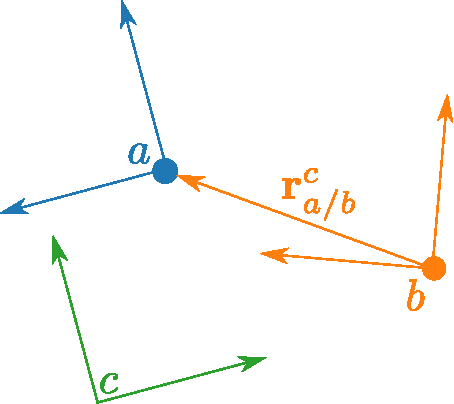
\includegraphics[width=\linewidth]{chap2_preliminaries/figures/frame}
\caption{Illustration of a vector with notation}
\label{fig:notation}
\end{marginfigure}

Although it may be sometimes hard to actually draw some quantities
clearly (like the angular rate of two coordinate frames), in engineering,
we typically define vectors as some quantity with respect to some
other reference. For example, the angular velocity of a rotating body
with respect to the earth might be written as $\omegabf_{b/E}$. While it
may be difficult to visualize, we could also consider the opposite
case, what the angular velocity of the earth was with respect to the
rotating body, $\omegabf_{E/b}$. It turns out that even in
this case, the ``earth-centric'' representation is just the negative
of the ``body-centric'' representation.
\[
\omegabf_{E/b}=-\omegabf_{b/E}.
\]

The next piece of information that we need is the frame of reference
it is described in (its basis). For example, in Figure~\ref{fig:notation},
we could describe $\rbf$ in any coordinate frame we want. We could
use frame $a$, $b$ or $c$, it doesn't really matter, so long as
we always do all operations between vectors represented in the same
frame.

We will use the superscript notation to describe the frame of reference,
as in $\rbf_{a/b}^{c}$.
\sidenote{In words $r_{a/b}^c$ means ``the position of frame $a$ with respect to
frame $b$, expressed in frame $c$.''} All vectors have this concept
of frame of reference, even if they are hard to visualize, like angular
rate, acceleration, etc...

%-------------------------------------------------------------
\subsection{A first look at rotation matrices.}
We can transform vector coordinates from one frame to another using a rotation matrix.  Let $R_a^b\in\mathbb{R}^{3\times 3}$ be the matrix that transforms the coordinates of physical vector expressed in frame $a$ to the coordinates of the same physical vector expressed in frame $b$.  
Note that $R_a^b$ will transform the coordinate axes of frame $a$ expressed in $a$ to the coordinate axes of frame $a$ expressed in $b$.  Therefore if we write $R_a^b$ in terms of its columns $R_a^b = \begin{pmatrix}\rbf_1 & \rbf_2 & \rbf_3 \end{pmatrix}$, then we have
\[
R_a^b \ibf_a^a =  \begin{pmatrix}\rbf_1 & \rbf_2 & \rbf_3 \end{pmatrix} \begin{pmatrix} 1 \\ 0 \\ 0 \end{pmatrix} 
= \rbf_1 
= \ibf_a^b.
\]
Using similar logic for the other columns we have
\[
R_a^b = \begin{pmatrix} \ibf_a^b & \jbf_a^b & \kbf_a^b \end{pmatrix}.
\]
\marginnote{The columns of the rotation matrix $R_a^b$ are the coordinate axes of frame $a$ expressed in frame $b$.}

Suppose that a vector $\rbf_{a/b}$ is expressed with respect to frame $c$ and we would like to express it with respect to frame $d$, then we can use the rotation matrix $R_c^d$ as the transformation
\[
\rbf_{a/b}^{d}=R_{c}^{d}\rbf_{a/b}^{c}
\]
\marginnote{The notation
is such that you can ``cancel out'' the frames, as in
\[
\rbf_{a/b}^{b}=R_{\cancel{c}}^{b}\mathbf{r}_{a/b}^{c}.
\]
Rotations can also be compounded as in 
\[
\rbf_{a/b}^{e}=R_{\cancel{d}}^{e}R_{\cancel{c}}^{\cancel{d}}\rbf_{a/b}^{\cancel{c}}.
\]
}
%
%Again, I'm deliberately skimming over most of the actual math. We'll
%get into this a lot more later, but we first need to get the mechanics
%of working with this notation.

%-----------------------------------------------------
\subsection{Vector composition.}
Recall that vector space is a collection of vectors and a scalar field with operations for vector addition and scalar multiplication.  The following table provides the definition for these operations.
%
%
%Let's now take a minute to remember what defines a vector space. From
%Wikipedia:
%\begin{quote}
%A vector space is a collection of objects called vectors, which may
%be added together and multiplied (\textquotedbl scaled\textquotedbl )
%by numbers, called scalars.
%\end{quote}
%All vector spaces abide by the following rules:
\begin{table}[ht]
\caption{Table of the rules of a Vector Space}
\begin{tabular}{cc}
\hline 
Axiom & Meaning\\
\hline 
\hline 
Associativity & $\abf+\left(\bbf+\cbf\right)=\left(\abf+\bbf\right)+\cbf$\\
\hline 
Commutativity & $\abf+\bbf=\bbf+\abf$
\\\hline 
Identity vector & 
	There exists a vector $\zerobf$ \\& 
	such that $\abf+\zerobf=\abf$ for \\&
	every vector in the space
\\\hline 
Inverse vector & 
	for every vector $\abf$, there is \\&
	 one and only one vector $-\abf$\\&
	such that \\&
	$\abf+\left(-\abf\right)=\zerobf.$
\\\hline 
distributivity of \\ scalar multiplication & 
	$\left(v+u\right)\abf=v\abf+u\abf$ \\&
	$v\left(\abf+\bbf\right)=v\abf+v\bbf$
\\\hline 
Identity scalar & $1\abf=\abf$\tabularnewline
\hline 
\end{tabular}
\end{table}

Physical vectors are part of the 3D Euclidian vector space $\mathbb{E}^3$ the scalar field being given by the real numbers $\mathbb{R}$.  This will be in contrast to rotation matrices that are not elements of a vector space.  Later in this chapter we will define the notion of a group, which will be much more useful in dealing with rotation matrices.

%
%\begin{flushleft}
%If you've taken a course in linear algebra, these will not be new
%to you. However, for me, up to this point, I had never worked with
%objects that were \emph{not }in a vector space, so the rules seemed
%obvious and redundant.
%\par\end{flushleft}

We like vector spaces because computers are well-suited for solving
linear algebra problems. There are high-performance BLAS libraries
(basic linear algebra subprograms) and methods for performing matrix
decompositions (SVD, LU, QR, Cholesky etc...) that allow us to solve
complicated problems quickly and accurately. 

It turns out that rotations and transformations do \emph{not} lie
in a vector space. This means that we end up performing manipulations
to get our problems into a vector space where we can use powerful
linear algebra techniques, and the distinction between vector spaces
and non-vector spaces will become very important.

\begin{marginfigure}
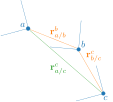
\includegraphics[width=\linewidth]{chap2_preliminaries/figures/vector_composition}
\caption{Illustration of a vector triangle}
\label{fig:vector_compose}
\end{marginfigure}
Figure~\ref{fig:vector_compose} shows three coordinate frames $a$, $b$, and $c$.
We would like to add the orange vectors $\rbf_{b/c}^c$ and $\rbf_{a/b}^b$.  
Vector addition applies, but only if the vectors are expressed in the same coordinate frame.  Therefore, to add the vectors we must first transform $\rbf_{a/b}^b$ into frame $c$ to get
\[
\rbf_{a/c}^{c}=\rbf_{b/c}^c + R_{b}^{c}\rbf_{a/b}^b.
\]
%
%
% as shown in Figure \ref{fig:vector_compose}.
%Let's also say that we have only the orange vectors. (the vector from
%$b\to a$ and the vector from $c\to b$) but we want the green vector
%(the one that goes all the way from $c\to a$).
%
%
%Well, this would be easy if they were all represented in the same
%coordinate frame
%
%\[
%\rbf_{a/c}=\rbf_{a/b}+\rbf_{b/c},
%\]
%but they aren't. However, we just have to remember that vectors can
%only be added or subtracted if they are in the same frame, so we just
%rotate them into a common frame before doing the additions, like this:
%
%\[
%\rbf_{a/c}^{c}=R_{b}^{c}\left(\rbf_{b/c}^{b}+R_{a}^{b}\rbf_{a/b}^{a}\right).
%\]
%From a theoretical perspective, the choice of coordinate frame doesn't
%matter, however in practice there is often a choice of frame that
%makes things easier.


%-----------------------------------------------------
\subsection{Cross product and skew symmetric matrices.}
The cross product of two vectors in $\mathbb{R}^3$ is defined as
\[
\begin{pmatrix} a_1 \\ a_2 \\ a_3 \end{pmatrix} \times \begin{pmatrix} b_1 \\ b_2 \\ b_3 \end{pmatrix} = \begin{pmatrix} a_2 b_3 - a_3 b_2 \\ a_3 b_1 - a_1 b_3 \\ a_1 b_2 - a_2 b_2 \end{pmatrix}.
\]
Direct manipulation shows that cross product satisfies the following identities:
\begin{align}
\abf \times \bbf = -\bbf \times \abf \label{eq:cross_product_1} \\
\abf \times (\bbf \times \cbf) = \abf^\top \cbf \bbf - \abf^\top\bbf \cbf \label{eq:cross_product_2} \\
\abf^\top(\bbf\times\cbf)=\cbf^\top(\abf\times\bbf)=\bbf^\top(\cbf\times\abf) \label{eq:cross_product_3} \\
(\abf\times\bbf)^\top(\cbf\times\dbf) = (\abf^\top\cbf)(\bbf^\top\dbf)-(\abf^\top\dbf)(\bbf^\top\cbf) \label{eq:cross_product_4} \\
\norm{\abf \times \bbf} = \norm{\abf}\norm{\bbf}\sin\phi, \quad \phi=\text{angle between $\abf$ and $\bbf$}\label{eq:cross_product_5} \\
\abf^\top (\bbf\times\cbf) = \text{det}\{\begin{pmatrix}\abf & \bbf & \cbf\end{pmatrix}\}. \label{eq:cross_product_6}
\end{align}
If $R$ is a rotation matrix, then 
\begin{equation} \label{eq:cross_product_7}
R(\abf\times\bbf) = (R\abf)\times(R\bbf).	
\end{equation}


It is straight forward to show that for any $\abf,\bbf\in\mathbb{R}^3$, 
\marginnote{The ``wedge'' operator is defined in Equation~\eqref{eq:wedge}.}  
\[
\ss{\abf}\bbf = \abf\times\bbf.
\]
Therefore $\ss{\abf}$ is a matrix implementation of the cross product operation.
From the properties of the cross product, we can derive the following properties for skew symmetric matrices:
\begin{align}
\ss{\abf} = -\ss{\abf}^\top \label{eq:skew_matrix_1}\\
\ss{\abf}\ss{\bbf} = \bbf\abf^\top - (\abf^\top\bbf)I \label{eq:skew_matrix_2}\\
\abf^\top\ss{\bbf} = (\ss{\abf}\bbf)^\top = -\bbf^\top\ss{\abf} \label{eq:skew_matrix_3}\\
(\ss{\abf}\bbf)^\top\ss{\cbf} = \abf^\top(\cbf\bbf^\top-\bbf^\top\cbf I).\label{eq:skew_matrix_4}
\end{align}
From property~\eqref{eq:skew_matrix_2}, we have that if $\nbf$ is a unit vector, then
\begin{equation}\label{eq:skew_matrix_5}
\ss{\nbf}^2 = \nbf\nbf^\top-I.
\end{equation}
\marginnote{
\begin{align*}
&R(\abf\times\bbf)=(R\abf)\times(R\bbf) \\
\iff & R\ss{\abf}\bbf = \ss{R\abf}R\bbf \\
\iff & R\ss{\abf} = \ss{R\abf}R \\
\iff & R\ss{\abf}R^\top = \ss{R\abf}
\end{align*}
}
From property~\eqref{eq:cross_product_7} we have
\begin{equation}\label{eq:skew_matrix_6}
\ss{R\abf} = R\ss{\abf}R^\top.
\end{equation}

Define the symmetric and skew-symmetric operators as
\begin{align}
\mathbb{P}_s (A) &\defeq \frac{1}{2}(A+A^\top) \label{eq:symmetric_operator} \\
\mathbb{P}_a (A) &\defeq \frac{1}{2}(A-A^\top), \label{eq:skew_symmetric_operator}
\end{align}
and note that $A=\mathbb{P}_s(A)+\mathbb{P}_a(A)$.  Therefore, any square matrix $A$ can be decomposed into a symmetric part, and a skew-symmetric part.

%++++++++++++++++++++++++++++++++++++++++++++++++++++++++++++
\subsection{Useful matrix identities}
In this section, we collect some useful matrix identities.

The trace of a matrix $A=\{a_{ij}\}\in\mathbb{R}^{m\times n}$ is defined as the sum of the the diagonal terms, i.e.,
\[
\trace{A} = \sum_{i=1}^{\min(m,n)} a_{ii}.
\]
The following properties of the trace of a matrix well known, where it is assumed that matrices have compatible dimensions:
\begin{align}
\trace{A^\top} =\trace{A}, \label{eq:trace_property_1} \\
\trace{AB} = \trace{BA}, \label{eq:trace_property_2} \\
\trace{\alpha A + \beta~B} = \alpha~\trace{A} + \beta~\trace{B}, \label{eq:trace_property_3} \\
A-\text{symmetric}, B-\text{skew symmetric} \implies \trace{AB} = 0, \label{eq:trace_property_4} \\
\trace{\ss{\abf} \ss{\bbf}} = -2\abf^\top \bbf. \label{eq:trace_property_5}
\end{align}


The Frobenius norm of matrix $A=\{a_{ij}\}\in\mathbb{R}^{n\times n}$ is defined as
\[
\norm{A}_F \defeq \sqrt{\trace{A^\top A}} = \sum_{ij} \abs{a_{ij}}^2.
\]
\begin{lemma} \label{lem:norm_to_trace}
If $R\in SO(3)$, then 
\begin{equation}\label{eq:frobenius_norm_to_trace}
\norm{I-R}_F^2 = 2~\trace{I-R}.
\end{equation}
\end{lemma}
\begin{proof}
\begin{align*}
\norm{I-R}_F^2 &= \trace{(I-R)^\top(I-R)} \\
  	&= \trace{I - R - R^\top + R^\top R}.
\end{align*}
Since $R\in SO(3)$ we have that $R^\top R = I$.  Therefore from properties~\eqref{eq:trace_property_1} and \eqref{eq:trace_property_3} we get Equation~\eqref{eq:frobenius_norm_to_trace}.
\end{proof}


%+++++++++++++++++++++++++++++++++++++++++++++++++++++++++++++
\section{The Rodrigues Formula}
\label{sec:rodrigues_formula}

In this section we derive the so-called {\em Rodrigues Formula} that describes a right handed rotation of angle $\theta$ about a vector $\mathbf{n}$. 
We will use this formula throughout the book. Our derivation
follows that given in {\em Stevens \& Lewis}~\cite{StevensLewis03}.  Consider the geometry shown in Figure~\ref{fig:rotation_formula}, where the vector $\mathbf{q}$ is obtained by a right-handed rotatation of the vector $\mathbf{p}$ about the unit vector $\mathbf{n}$ by an angle of $\theta$. 
%
\begin{marginfigure}[-5in]
  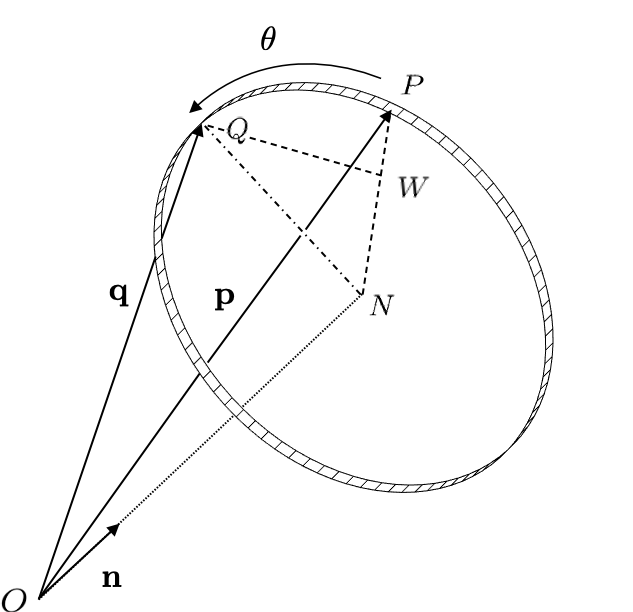
\includegraphics[width=\linewidth]{chap2_preliminaries/figures/rotation_formula}\\
  \caption{Right-handed rotation of a vector $\mathbf{p}$ about the unit
  vector $\mathbf{n}$ by an angle of $\theta$ to obtain the vector $\mathbf{q}$.}
  \label{fig:rotation_formula}
\end{marginfigure}
%
From the geometry, note that 
\begin{equation}\label{eq:frames-rot-formula-prelim}
\mathbf{q} = \vec{ON} + \vec{NW} + \vec{WQ}.
\end{equation}
The vector $\vec{ON}$ can be found by taking the projection of
$\mathbf{p}$ on the unit vector $\mathbf{n}$ in the direction of
$\mathbf{n}$, giving
\[
\vec{ON} = \left(\pbf\cdot\nbf\right)\nbf = (\nbf \nbf^\top) \pbf.
\]
The vector $\vec{NW}$ is in the direction of $\mathbf{p}-\vec{ON}$
with a length of $\norm{\vec{NQ}}\cos\theta$.  Noting that the length $NQ$ equals
the length $NP$ which is equal to $\norm{\mathbf{p}-\vec{ON}}$ we
get that
\begin{align*}
\vec{NW} &= \frac{\pbf-\left(\pbf \cdot \nbf\right)\nbf}
{\norm{\pbf-\left(\pbf\cdot\nbf\right)\nbf}}
\norm{\vec{NQ}}\cos\theta
\\
&=
\cos\theta\left(I-\nbf\nbf^\top\right)\pbf.
\end{align*}
The vector $\vec{WQ}$ is perpendicular to both $\mathbf{p}$ and
$\mathbf{n}$ and has length $\norm{\vec{NQ}}\sin\theta$.  Noting that
$\norm{\vec{NQ}}=\norm{\mathbf{p}}\sin\phi$ and that $\norm{\nbf\times\pbf}=\norm{\pbf}\sin\phi$, where $\phi$ is the angle between $\nbf$ and $\pbf$, we get
\begin{align*}
\vec{WQ} &=
\frac{\nbf\times\pbf}{\norm{\nbf\times\pbf}}\norm{\vec{NQ}}\sin\theta
\\
&= \mathbf{n}\times\mathbf{p}\sin\theta \\
&= \sin\theta \ss{\nbf}\pbf.
\end{align*}
Therefore Equation~\eqref{eq:frames-rot-formula-prelim} becomes
\[
\mathbf{q} = \left(\nbf \nbf^\top + \cos\theta (I-\nbf\nbf^\top) + \sin\theta \ss{\nbf} \right)\pbf.
\]
Let
\[
R(\nbf,\theta)=\nbf \nbf^\top + \cos\theta (I-\nbf\nbf^\top) + \sin\theta \ss{\nbf},
\]
and note that using Equation~\eqref{eq:skew_matrix_5} we can write
\marginnote{Equation~\eqref{eq:skew_matrix_5} is $(\ss{\nbf})^2 = \nbf\nbf^\top-I$.}
\begin{equation}\label{eq:rodrigues_1}
R(\nbf,\theta)=I + \sin\theta \ss{\nbf} + (1-\cos\theta)\ss{\nbf}^2,
\end{equation}
which is called the Rodrigues formula.
As described in the next section, we will often use angle-axis notation to define rotations.  In angle-axis notation, the rotation vector is given by
$\abf=\theta\nbf$.  Therefore, we will typically write the Rodrigues formula as 
\begin{equation}\label{eq:rodigues_2}
	R(\theta\nbf) = I + \sin\theta \ss{\nbf} + (1-\cos\theta)\ss{\nbf}^2.
\end{equation}
Note that for any vector $\abf$ we have $\abf=\norm{\abf}\frac{\abf}{\norm{\abf}}$.  Equating $\theta$ with $\norm{\abf}$ and $\nbf$ with the unit vector $\abf/\norm{\abf}$, the Rodrigues formula becomes
\marginnote{We have used the identity $1-\cos x = 2\sin^2(x/2)$ to get $\frac{1-\cos x}{x^2} = \frac{1}{2}\sinc^2(x/2)$, where $\sinc(x)=\frac{\sin(x)}{x}$.}
\begin{align}
R(\abf) &= I + \left(\frac{\sin\norm{\abf}}{\norm{\abf}}\right)\ss{\abf} + \left(\frac{1-\cos\norm{\abf}}{\norm{\abf}^2}\right)\ss{\abf}^2 \notag \\
		&= I + \sinc(\norm{\abf})\ss{\abf} + \frac{1}{2}\sinc^2\left(\frac{\norm{\abf}}{2}\right)\ss{\abf}^2.
		\label{eq:rodrigues_2}
\end{align}

As an illustration of the Rodrigues formula, we get that a rotation of $\phi$ about the vector $\ebf_1=(1,0,0)^\top$ is
\begin{align*}
R(\ebf_1,\phi) &= I + \sin\phi \ss{\ebf} + (1-\cos\phi)\ss{\ebf_1}^2	\\
&= \begin{pmatrix}1 & 0 & 0 \\ 0 & 1 & 0 \\ 0 & 0 & 1 \end{pmatrix}
   +\sin\phi \begin{pmatrix} 0 & 0 & 0 \\ 0 & 0 & -1 \\ 0 & 1 & 0\end{pmatrix} 
   + (1-\cos\phi)\begin{pmatrix}0 & 0 & 0 \\ 0 & -1 & 0 \\ 0 & 0 & -1 \end{pmatrix} \\
&= \begin{pmatrix} 1 & 0 & 0 \\ 0 & \cos\phi & -\sin\phi \\ 0 & \sin\phi & \cos\phi \end{pmatrix}.
\end{align*}
Similarly, the Rodrigues formula gives that rotations by $\theta$ about $\ebf_2$ and $\psi$ about $\ebf_3$ are
\begin{align*}
R(\ebf_2, \theta) &= \begin{pmatrix} \cos\theta & 0 & \sin\theta \\ 0 & 1 & 0 \\ -\sin\theta & 0 & \cos\theta \end{pmatrix} \\
R(\ebf_3, \psi) &= \begin{pmatrix} \cos\psi & -\sin\psi & 0 \\ \sin\psi & \cos\psi & 0 \\ 0 & 0 & 1 \end{pmatrix} \\
\end{align*}

One may wonder if all rotation can be described by the Rodrigues formula.  It turns out that Leonhard Euler proved in 1775 the following theorem.
\sidenote{\url{https://en.wikipedia.org/wiki/Euler\%27s_rotation_theorem}.}
\begin{theorem}[Euler's Rotation Theorem]
	In three dimensional space, any sequence of rotations is equivalent to a single rotation about a fixed vector.
\end{theorem}
Therefore, any rotation and any sequence of rotations, can be represented by a single rotation matrix with some angle $\theta$ and some unit vector $\nbf$, where the corresponding rotation is $R(\nbf,\theta)$.
It turns out that the eigenvalues and eigenvectors of any rotation $R(\nbf,\theta)$ can be derived analytically.
\begin{lemma}
Given a rotation matrix $R(\nbf,\theta)$ the eigenvalues are $\lambda=1, \exp(j\theta), \exp(-j\theta)$, with corresponding eigenvectors
$\nbf$, $\nbf_2+j\nbf_3$, and $\nbf_2-j\nbf_3$, where $\{\nbf, \nbf_2, \nbf_3\}$ form a right handed coordinate frame.
\end{lemma}
\begin{proof}
From the Rodrigues formula we get
\marginnote{We have used the fact that $\nbf\times\nbf=0$ implies that $\ss{\nbf}\nbf = 0$.}
\[
R(\nbf,\theta)\nbf = \nbf + \sin\theta \ss{\nbf}\nbf + (1-\cos\theta)\ss{\nbf}\ss{\nbf}\nbf
                   = 1\cdot\nbf.
\]
Therefore $\lambda=1$ is an eigenvector of $R(\nbf,\theta)$ with eigenvector $\nbf$.  Pick any $\nbf_2$ that is orthogonal to $\nbf$, and let $\nbf_3=\ss{\nbf}\nbf_2$ so that $\{\nbf, \nbf_2, \nbf_3\}$ form a right-handed coordinate system.  Then
\begin{align*}
	R(\nbf,\theta)\nbf_2 &= \nbf_2 + \sin\theta \ss{\nbf}\nbf_2 + (1-\cos\theta)\ss{\nbf}\ss{\nbf}\nbf_2 \\
	&= \nbf_2 + \sin\theta \nbf_3 - (1-\cos\theta)\nbf_2 \\
	&= \cos\theta \nbf_2 + \sin\theta \nbf_3.
\end{align*}
Similarly, it is straightforward to show that $R(\nbf,\theta)\nbf_3 = \cos\theta \nbf_3 - \sin\theta \nbf_2$.  Therefore
\begin{align*}
	R(\nbf,\theta)(\mathbf{n}_2 \pm j\mathbf{n}_3) &= (\cos\theta\mathbf{n}_2 + \sin\theta\mathbf{n}_3) \pm j(\cos\theta \mathbf{n}_3 - j\sin\theta\mathbf{n}_2) \\
		&= (\cos\theta \pm j\sin\theta)\mathbf{n}_2 \mp j(\cos\theta \pm j\sin\theta)\mathbf{n}_3 \\
		&= e^{\pm j\theta} (\mathbf{n}_2 \mp j\mathbf{n}_3).
\end{align*}
Therefore, the other two eigenvectors are $\mathbf{n}_2\pm j\mathbf{n}_3$ with associated eigenvalues of $e^{\mp j\theta}$.  
Conversely, it can be shown that all rotation matrices have a similar eigen-structure.  Therefore, every rotation matrix $R\in SO(3)$ will have eigenvalues of $1$ and $e^{\mp j\theta}$, and $R$ can be visualized as rotating a vector $\mathbf{p}$ by a left-handed rotation of angle $\theta$ about the eigenvector $\mathbf{n}$ associated with eigenvalue $1$. 
\end{proof}
It is standard convention to call $\nbf$ the eigen-axis of rotation.  

The Rodrigues formula also gives the following result for the trace of $R$.
\begin{lemma}\label{lem:prelim-trace-of-R}
For any $R(\nbf,\theta)\in SO(3)$ we have
\[
\trace{R} = 1+2\cos\theta.
\]	
\end{lemma}
\begin{proof}
Since $\ss{\nbf}^2 = \nbf \nbf^\top  - I$, we get that
\begin{align*}
\trace{R} &= \trace{I} + \sin\theta~\trace{\ss{\nbf}} + (1-\cos\theta)\trace{\nbf \nbf^\top - I} \\
          &= 3 + \sin\theta \cdot 0 + (1-\cos\theta)(n_1^2+n_2^2+n_3^2 - 3) \\
          &= 1 + 2\cos\theta,
\end{align*}
where $\nbf=(n_1, n_2, n_3)^\top$.
\end{proof}

We conclude this section by deriving an extremely useful expression for the Rodrigues formula.  Recall from linear algebra, that the exponential of a square matrix $A\in\mathbb{R}^{n\times n}$ is defined as
\begin{equation}\label{eq:matrix_exponential}
e^{A} = \exp(A) = I + A + \frac{1}{2!}A^2 + \frac{1}{3!}A^3 + \frac{1}{4!}A^4 + \dots.
\end{equation}
\begin{lemma}\label{lem:rodrigues_exponential}
For any unit vector $\nbf$ and scalar $\theta$,
\[
R(\nbf,\theta) = \exp(\theta\ss{\nbf}).
\]	
\end{lemma}
\begin{proof}
From Equation~\eqref{eq:skew_matrix_5} we have that
\begin{align*}
	\ss{\nbf}^3 &= \ss{\nbf}(\nbf\nbf^\top-I) \\
	            &= -\ss{\nbf},
\end{align*}
implying that for $m=0, 1, 2, \dots$, $\ss{\nbf}^{(2m+1)} = (-1)^m\ss{\nbf}$.
Therefore $\ss{\nbf}^4=-\ss{\nbf}^2$, implying that for $m=0, 1, 2, \dots$, 
$\ss{\nbf}^{(2m+2)} = (-1)^m\ss{\nbf}^2$. Using Equation~\eqref{eq:matrix_exponential} we get
\begin{align*}
\exp(\theta \ss{\nbf}) &= I + \theta \ss{\nbf} + \frac{\theta^2}{2!}\ss{\nbf}^2 + \frac{\theta^3}{3!}\ss{\nbf}^3 + \frac{\theta^4}{4!}\ss{\nbf}^4
                          + \dots \\
                      &= I + \theta \ss{\nbf} + \frac{\theta^2}{2!}\ss{\nbf}^2 - \frac{\theta^3}{3!} \ss{\nbf} - \frac{\theta^4}{4!}\ss{\nbf}^2 +\dots \\
                      &= I + \left(\theta - \frac{\theta^3}{3!} + \frac{\theta^5}{5!} - \dots \right)\ss{\nbf} + \left(\frac{\theta^2}{2!} - \frac{\theta^4}{4!} + \dots\right)\ss{\nbf}^2 \\
                      &= I + \sin\theta\ss{\nbf} -(\cos\theta -1)\ss{\nbf}^2 \\
                      &= R(\nbf, \theta).
\end{align*}
\end{proof}

We can also define the $\log$ of a rotation matrix as the inverse operation, where we require that $\log(\exp(R))=R$.
\begin{lemma}\label{lem:matrix_log}
Given any $R\in SO(3)$, the logarithm of $R$ is given by
\[
\log(R) = \frac{1}{2}\frac{R-R^\top}{\sinc{\theta}}
\]
where
\[
\theta = \cos^{-1}\left(\frac{\trace{R}-1}{2}\right).
\]
%\[
%\log(R) = \left(\frac{\cos^{-1}\left(\frac{\trace{R}-1}{2}\right)}{\sqrt{(3-\trace{R})(1+\trace{R})}}\right)(R-R^\top).
%\]
\end{lemma}
\begin{proof}
Euler's rotation theorem implies that there exist $\nbf$ and $\theta$ such that $R=\exp(\theta\ss{\nbf})$.  Therefore
\[
\log(R) = \log(\exp(\theta\ss{\nbf}))=\theta\ss{\nbf}.
\]
From Lemma~\ref{lem:prelim-trace-of-R} we have that
\[
\theta = \cos^{-1}\left(\frac{\trace{R}-1}{2}\right).
\]
Using the Rodrigues formula we have
\sidenote{We have used the fact that $\ss{\nbf}^\top = -\ss{\nbf}$ and $\ss{\nbf}^{\top 2} = \ss{\nbf}^2$.}
\begin{align*}
R - R^\top &= I + \sin\theta \ss{\nbf} + (1-\cos\theta)\ss{\nbf}^2 \\
		   &\qquad - I^\top - \sin\theta\ss{\nbf}^\top - (1-\cos\theta)\ss{\nbf}^{\top 2} \\
           &= 2\sin\theta \ss{\nbf},
\end{align*}
which implies that \sidenote{Note that this formula shows that an equivalent expression for the logarithm or $R$ is $\log(R) = \frac{1}{2}\frac{R-R^\top}{\sinc\theta}$ where $\sinc\theta = \frac{\sin\theta}{\theta}$.}
\[
\ss{\nbf} = \frac{R-R^\top}{2\sin\theta}.
\]
Therefore
\[
\log{R} = \theta\ss{\nbf} = \theta\frac{R-R^\top}{2\sin\theta} = \frac{1}{2}\frac{R-R^\top}{\sinc{\theta}}.
\]
%
%Using the fact that $\sin(\cos^{-1}(x))=\sqrt{1-x^2}$ gives
%\[
%\sin\left(\cos^{-1}\left(\frac{\trace{R}-1}{2}\right)\right) = \frac{\sqrt{(3-\trace{R})(1+\trace{R})}}{2},
%\]
%which gives the result.
\end{proof}


%-------------------------------------------------------------
\section{Attitude Representation}
\label{sec:attitude_representation}

In this section we describe four different attitude representations that will be used in the book.  The attitude or orientation of a multirotor can be described using Euler angles, a rotation matrix, a unit quaternion, or using a rotation vector, which is often called angle-axis representation.  The following subsection will describe each of these conventions and how they are used to describe the attitude of a multirotor, and the attitude of an attached camera.  We will find that each of these representations are convenient for different aspects of vision-based estimation and control, and so we also describe how to transform between the different representations.

%+++++++++++++++++++++++++++++++++++++++++++++++++++++++++++++
\subsection{Euler Angles}

The most common representation for attitude is the 3-2-1 Euler angles, often called the aircraft yaw, pitch, and roll angles.  
The body frame of a multirotor is defined as $\mathcal{F}_b = \{\ibf_b, \jbf_b, \kbf_b\}$.  The body $\ibf_b$-axis is in a plane parallel to the rotors, and points in a direction that is designated as the forward-direction for the multirotor. The body $\kbf_b$-axis is perpendicular to the rotor plane, and points opposite the direction of thrust, designated as the body down direction.  The body $\jbf_b$-axis is so that $\jbf=\kbf\times\ibf$ and points to the right in the body.

The yaw angle of a multirotor is defined as a right-handed rotation about the inertial $\kbf_i$ axis, as shown in Figure~\ref{fig:quadrotor_yaw}.  The resulting intermediary frame is called the body-1 frame in \cite{BeardMcLain12}.  The yaw angle is designated as $\psi$.
\begin{marginfigure}
  \centering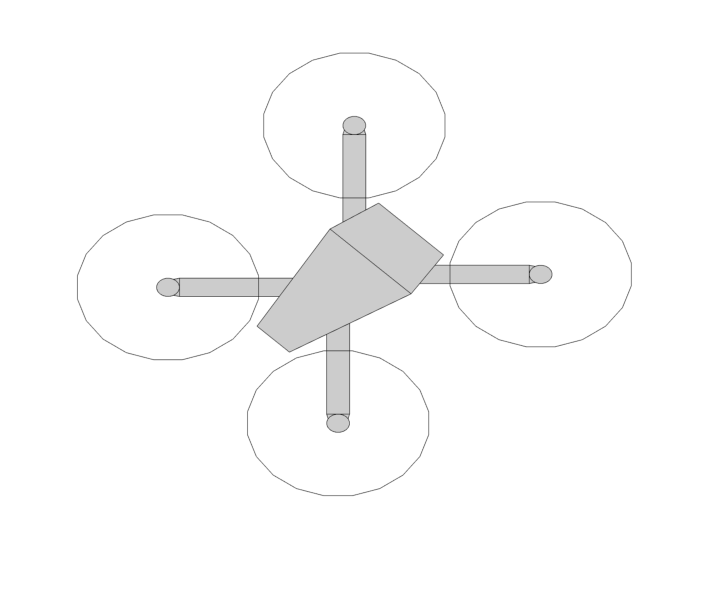
\includegraphics[width=\linewidth]{chap2_preliminaries/figures/quadrotor_yaw}
  \caption{The yaw angle is defined as a right-handed rotation about the inertial $\kbf_i$ axis.}
  \label{fig:quadrotor_yaw}  
\end{marginfigure}
%
The pitch angle of a multirotor is defined as a right-handed rotation about the $\jbf_1$ in the body-1 frame, as shown in Figure~\ref{fig:quadrotor_pitch}, and the resulting intermediary frame is called the body-2 frame in~\cite{BeardMcLain12}. The pitch angle is designated as $\theta$.
\begin{marginfigure}
  \centering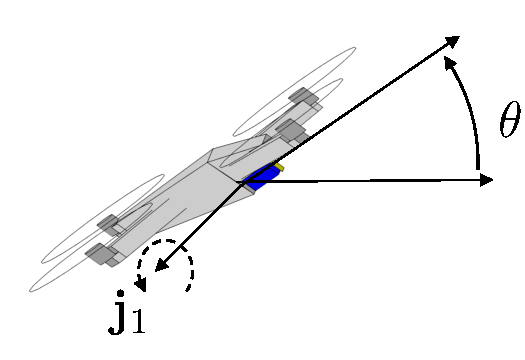
\includegraphics[width=\linewidth]{chap2_preliminaries/figures/quadrotor_pitch}
  \caption{The pitch angle is defined as a right-handed rotation about the body-1 $\jbf$ axis.}
  \label{fig:quadrotor_pitch}  
\end{marginfigure}
%
The roll angle of a multirotor is defined as a right-handed rotation about the body-2 $\ibf_2$ axis, as shown in Figure~\ref{fig:quadrotor_roll}.  The roll angle is designated as $\phi$.
\begin{marginfigure}
  \centering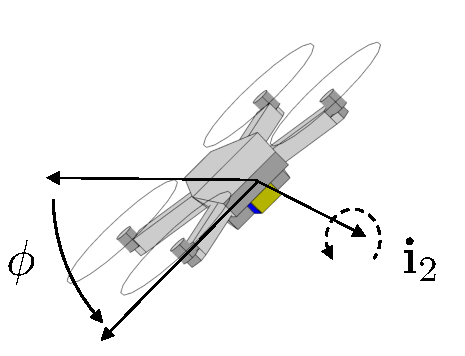
\includegraphics[width=\linewidth]{chap2_preliminaries/figures/quadrotor_roll}
  \caption{The roll angle is defined as a right-handed rotation about the body-2 $\ibf_2$ axis.}
  \label{fig:quadrotor_roll}  
\end{marginfigure}
Throughout the book, we will designate the vector of Euler angles by 
\[
\Theta = \begin{pmatrix} \phi \\ \theta \\ \psi \end{pmatrix}.
\]

Euler angle are often used because they are intuitive to understand and easy to visualize.  When attitude needs to be plotted in a graph, the Euler angles are typically used for convenience.  However, Euler angles represent a local representation of attitude and are rarely suitable for simulation, estimation, or control.  First note that Euler angles do not commute, i.e., a yaw followed by a pitch followed by a roll, is different than a roll followed by a pitch followed by a yaw.  This non-commutivity has many negative implications.  To understand that they are a local representation, consider the attitude that would result by first pitching the multirotor by 90 degrees, and then rolling by 90 degrees.  This is the same orientation that would result from first yawing by 90 degrees, and then pitching by 90 degrees.  Therefore Euler angle representations do not uniquely represent the attitude.


The pointing angle, or attitude of the camera relative to the multirotor can be describe by the azimuth and elevation angles.  
%
The azimuth angle of the camera is defined as a right-handed rotation about the multirotor body $\kbf_b$ axis, as shown in Figure~\ref{fig:quadrotor_azimuth}.  The resulting intermediary frame is called the gimbal-1 frame in \cite{BeardMcLain12}.  The azimuth angle is designated in this book as $\alpha$.
\begin{marginfigure}
  \centering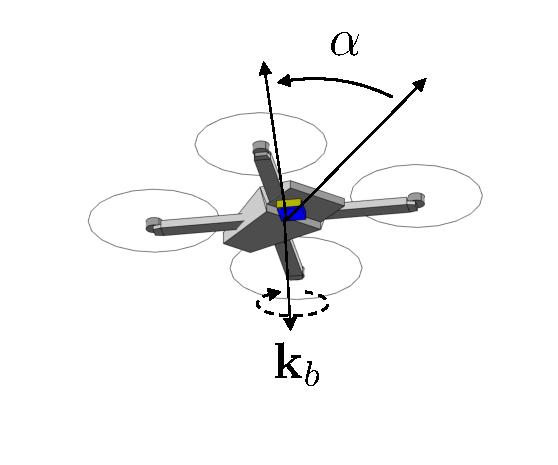
\includegraphics[width=\linewidth]{chap2_preliminaries/figures/quadrotor_azimuth}
  \caption{The azimuth angle of the camera is defined as a right-handed rotation about the multirotor body $\kbf_b$ axis.}
  \label{fig:quadrotor_azimuth}  
\end{marginfigure}
%
The elevation angle of the camera is defined as a right-handed rotation about the gimbal-1 $\jbf_{g1}$ axis, as shown in Figure~\ref{fig:quadrotor_elevation}.  The resulting frame is called the gimbal frame.  The elevation angle is designated in this book as $\beta$.
\begin{marginfigure}
  \centering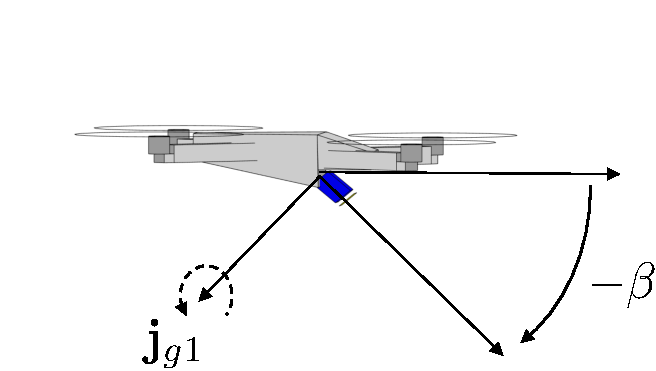
\includegraphics[width=\linewidth]{chap2_preliminaries/figures/quadrotor_elevation}
  \caption{The elevation angle of the camera is defined as a right-handed rotation about the gimbal-1 $\jbf_{g1}$ axis.}
  \label{fig:quadrotor_elevation}  
\end{marginfigure}


\subsection{Rotation Matrices}

As discussed previously, the attitude of a multirotor can also be represented by a rotation matrix.
A matrix $M\in\mathbb{R}^{n\times n}$ is said to be {\em orthogonal} if $MM^\top = M^\top M=I$, or equivalently if $M^{-1} = M^\top$.  The set of $n$-dimensional orthogonal matrices are designated by 
\[
O(n) = \{ M\in\mathbb{R}^{n\times n} | M^{-1}=M^\top \}.
\]
If $M=(\mbf_1, \mbf_2, \dots, \mbf_n)\in O(n)$, then 
\[
M^\top M =\begin{pmatrix} \mbf_1^\top \mbf_1 & \dots & \mbf_1^\top \mbf_n \\
\vdots & & \vdots \\
\mbf_n^\top \mbf_1 & \dots & \mbf_n^\top \mbf_n \end{pmatrix}=I
\]
implies that the columns of $M$ are orthogonal to each other and have unit length.  From properties of the determinate $\text{det}(M^\top)=\text{det}(M)$ and $\text{det}(I)=1$, we have that
\begin{align*}
& \text{det}(M^\top M) = \text{det}(I) \\
\iff & \text{det}^2(M) = 1 \\
\iff & \text{det}(M) = \pm 1.	
\end{align*}
For $3\times 3$ matrices, Equation~\eqref{eq:cross_product_6} implies that $\text{det}(M)=\mbf_1^\top(\mbf_2\times\mbf_3)$.  Therefore $\text{det}(M)=1$ if and only if the columns of $M$ form a right-handed coordinate system ($\mbf_2\times\mbf_3=\mbf_1$), otherwise the determinant is equal to $-1$.  
Therefore we define the set of special orthogonal matrices 
\[
SO(n) = \{M\in\mathbb{R}^{n\times n} | M\in O(n) \text{~and~} \text{det}(M)=1 \},
\]
and note that $R\in SO(3)$ implies that the columns of $R$ form a right-handed coordinate system.  Therefore, there is a one-to-one relationship between the orientation of right-handed coordinate systems and elements of $SO(3)$.  We say that $R$ is a rotation matrix if $R\in SO(3)$.  Note that the set $SO(3)$ does not form a vector space since $aR_1+bR_2\not\in SO(3)$ when $R_1,R_2\in SO(3)$.  We will see later that elements of $SO(3)$ form a {\em group}, and which is called the {\em special orthgonal group of order 3}.

Therefore, the orientation of a multirotor can be represented by an element of $SO(3)$.  If $\mathcal{F}_b = \{\ibf_b, \jbf_b, \kbf_b\}$ is a right-handed coordinate frame fixed in the multirotor body, then the attitude of $\mathcal{F}_b$ relative to another frame $\mathcal{F}_a = \{\ibf_a, \jbf_a, \kbf_a\}$ is given by
\[
R_b^a = \begin{pmatrix} \ibf_b^a & \jbf_b^a & \kbf_b^a \end{pmatrix}
\]
where the columns of $R_a^b$ are the unit vectors of frame $\mathcal{F}_b$ expressed relative to frame $\mathcal{F}_a$.  We will be particularly interested in $R_b^i$, the attitude of the multirotor body relative to the inertial frame, where $\ibf_b$ points out the nose of the multirotor, $\jbf_b$ points to the right, and $\kbf_b$ points down.  

To represent the attitude of the gimbal relative to the body, we need to assign a right-handed coordinate system to the gimbal.  Define $\mathcal{F}_g = \{\ibf_g, \jbf_g, \kbf_g\}$ such that $\ibf_g$ points along the optical axis of the camera, $\kbf_g$ points down when the gimbal is level, and $\jbf_g = \kbf_g\times\ibf_g$ points to the right.  The attitude of the gimbal relative to the body is given by
\[
R_g^b = \begin{pmatrix} \ibf_g^b & \jbf_g^b & \kbf_g^b \end{pmatrix}.
\]

To gain further insights into rotation matrices, note that any vector $\pbf$ can be represented in $\mathcal{F}_r$ and $\mathcal{F}_s$ as
\[
\pbf = \alpha_r\ibf_r + \beta_r\jbf_r + \gamma_r\kbf_r = \alpha_s\ibf_s + \beta_s\jbf_s + \gamma_s\kbf_s.
\]
Taking the inner product of both sides of this equation with the vectors $\ibf_r$, $\jbf_r$, and $\kbf_r$ gives
\begin{align*}
\alpha_r &= \alpha_s\ibf_r^\top \ibf_s + \beta_s\ibf_r^\top\jbf_s + \gamma_s\ibf_r^\top\kbf_s \\	
\beta_r &= \alpha_s\jbf_r^\top \ibf_s + \beta_s\jbf_r^\top\jbf_s + \gamma_s\jbf_r^\top\kbf_s \\
\gamma_r &= \alpha_s\kbf_r^\top \ibf_s + \beta_s\kbf_r^\top\jbf_s + \gamma_s\kbf_r^\top\kbf_s.
\end{align*}
Since $\pbf^r=(\alpha_r, \beta_r, \gamma_r)^\top$ and $\pbf^s=(\alpha_s, \beta_s, \gamma_s)^\top$ we have 
\[
\begin{pmatrix} \alpha_r \\ \beta_r \\ \gamma_r  \end{pmatrix} = 
\begin{pmatrix}
	\ibf_r^\top \ibf_s & \ibf_r^\top\jbf_s & \ibf_r^\top\kbf_s \\	
    \jbf_r^\top \ibf_s & \jbf_r^\top\jbf_s & \jbf_r^\top\kbf_s \\
    \kbf_r^\top \ibf_s & \kbf_r^\top\jbf_s & \kbf_r^\top\kbf_s
\end{pmatrix}
\begin{pmatrix}
	\alpha_s \\ \beta_s \\ \gamma_s
\end{pmatrix},
\]
\marginnote{The Cauchy-Schwartz equalty says that for any two vectors $\abf$ and $\bbf$, $\abf^\top \bbf = \norm{\abf}\norm{\bbf}\cos\theta$ where $\theta$ is the angle between $\abf$ and $\bbf$.}
or in other words $\pbf^r = R_s^r \pbf^s$, where we see that since $\nbf^\top\mbf=\cos\theta$ where $\theta$ is the angle between $\nbf$ and $\mbf$, that $R_s^r$ is a matrix of cosines of angles between the unit vectors of frame $r$ and frame $s$.  Therefore, rotation matrices are often called {\em direction cosine matrices.}  Therefore the vector
\[
\ibf_s^r = \begin{pmatrix}
 \text{angle between $\ibf_s$ and $\ibf_r$} \\	
 \text{angle between $\ibf_s$ and $\jbf_r$} \\	
 \text{angle between $\ibf_s$ and $\kbf_r$} \\	
 \end{pmatrix}.
\]

To emphasize some of the concept above, let $\mathcal{R}_r = \{\ibf_r, \jbf_r, \kbf_r\}$ and let $\mathcal{R}_s = \{\ibf_s, \jbf_s, \kbf_s\}$, 
then note that 
\[
\ibf_s^s = \begin{pmatrix} 1 \\ 0 \\ 0 \end{pmatrix}, \qquad 
\jbf_s^s = \begin{pmatrix} 0 \\ 1 \\ 0 \end{pmatrix}, \qquad 
\kbf_s^s = \begin{pmatrix} 0 \\ 0 \\ 1 \end{pmatrix}.
\]
Given the discussion above we have that
\[
R_s^r = \begin{pmatrix} \ibf_s^r & \jbf_s^r & \kbf_s^r \end{pmatrix},
\]
or 
\[
\ibf_s^r = R_s^r \ibf_s^s = \begin{pmatrix} \ibf_s^r & \jbf_s^r & \kbf_s^r \end{pmatrix} \begin{pmatrix} 1 \\ 0 \\ 0 \end{pmatrix}.
\]
Therefore the columns of $R_s^r$ are the unit axes of frame $\mathcal{F}_s$ expressed with respect to frame $\mathcal{F}_r$.

Let $\pbf_q$, $\pbf_r$ and $\pbf_s$ be the coordinates of $\pbf$ when expressed with respect to frames $\mathcal{F}_q$, $\mathcal{F}_r$, and $\mathcal{F}_s$, respectively. Then we can write
\begin{align*}
\pbf^r &= R_s^r \pbf^s \\
\pbf^q &= R_r^q \pbf^r.
\end{align*}
Therefore we have that $\pbf^q = R_r^q R_s^r \pbf^s$.  Since we also know that $\pbf_q = R_s^q \pbf_s$, we must have that
\[
R_s^q = R_r^q R_s^r.
\]

We have shown that rotation matrices satisfy the following properties
\begin{align}
& (R_r^s)^{-1} = (R_r^s)^T = R_s^r \label{eq:rotations_matrics_1} \\
& R_r^q R_s^r = R_s^q \label{eq:rotations_matrics_2} \\
& \det{R_r^s} = 1. \label{eq:rotations_matrics_3}
\end{align}

%+++++++++++++++++++++++++++++++++++++++++++++
\subsection{Passive Versus Active Rotations}

\begin{marginfigure}[-7in]
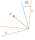
\includegraphics[width=0.8\linewidth]{chap2_preliminaries/figures/rotation_passive}
\caption{Illustration of a passive rotation.}
\label{fig:passive_rotation}
\end{marginfigure}

\begin{marginfigure}[-3in]
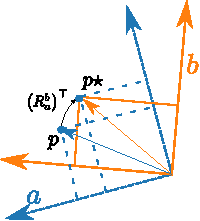
\includegraphics[width=0.8\linewidth]{chap2_preliminaries/figures/rotation_active}
\caption{Illustration of an active rotation.}
\label{fig:active_rotation}
\end{marginfigure}

We are using a convention here, where we define $R$ as a \emph{passive}
rotation. Consider Equation \ref{eq:rot_formula}. The vector quantity
$\rbf$ did not change during this rotation, it is simply being expressed
from another point of view. Some literature defines rotations as \emph{active}.
Figures~\ref{fig:passive_rotation} and~\ref{fig:active_rotation} illustrates the difference between
active and passive rotations. In the passive case, the point
$p$ does not change when rotating from frame $a$ to $b$. It remains
fixed while the perspective changes. In contrast, the active case, the point $p$ is moved to become a new object, point $\pbf^{\star}$.
This interpretation is much more common in the computer graphics literature,
where a common operation is to generate some asset at an arbitrary
origin, and then move that object to be rendered at some other location.
Engineering and robotics literature typically deal with passive rotations,
where the goal is often to reason about physical entities that are
not always directly controlled.

It can be shown that active and passive rotations are the transpose of
one another, as
\[
R_{active}=R_{passive}^{\top}.
\]
Throughout the book, we will always use passive rotations unless otherwise stated.

While rotation matrices are probably the most straight-forward method
to represent rotations, they have some shortcomings. The first is
that they require nine parameters to describe three degrees of freedom. This
causes larger memory requirements than strictly necessary, and requires
more operations than necessary when concatenating matrices.  With modern
computing resources, this is less of a problem, however the biggest
disadvantage is that numerical errors can accumulate in rotation matrices
and cause unwanted scaling and shearing as the matrix loses orthonormality.
This error can be corrected by Gram-Schmidt orthogonalization, but
doing so can be computationally expensive. As a result, rotation matrices
are still much more efficient than an Euler angle representation,
but they are not as efficient as unit quaternions.


%+++++++++++++++++++++++++++++++++++++++++++++++++++++++++++++
\subsection{Quaternions}

The material in this section loosely follows the notation in~\cite[-3in]{TrawnyRoumeliotis05}.

One of the disadvantages of rotation matrices is that they require nine parameters to represent a rotation, which is fundamentally a three dimensional entity.  Unit quaternions can be used to represent rotations using four parameters.  
Quaternions are hyper-complex numbers of the form 
\[
\mathbf{q} = q_0 + i q_x + j q_y + k q_z,
\]
where $i$, $j$, and $k$ are generalized complex numbers that satisfy 
\begin{equation}\label{eq:quaternion-complex-numbers}
i^2 = j^2 = k^2 = ijk = -1.
\end{equation}
\marginnote[-3in]{Because of the reverse order of concatenation, there is actually another
convention for quaternions, first used by NASA JPL, where the quaternion
imaginary numbers follow the \emph{left-hand} rule instead of the
right hand rule. This change makes unit quaternions concatenate right-to-left
(to match rotation matrices). The left-handed definition is known
as JPL notation, whereas the right-handed definition presented here
is known as Hamilton notation. While this change may seem innocent
on the surface, it has huge implications when we start talking about
Lie Groups. Modern scientific literature in robotics and computer
vision that use quaternions seem to almost always use Hamilton notation,
although JPL is used in some early quaternion papers relating to spacecraft
attitude observers.}

Equation~\eqref{eq:quaternion-complex-numbers} implies that $ijk^2=-k$ which implies that $ij=k$, which implies that $ij^2=kj$, which implies that $kj=-i$.  
By similar arguments we can show that $ij=-ji=k$, $jk=-kj=i$ and $ki=-ik=j$
Letting $\mathbf{p}=p_0 + ip_x + jp_y + kp_z$, we can multiply $\mathbf{p}$ and $\mathbf{q}$, and use the above relationships for $i, j, k$ to get
\begin{align}
\mathbf{p}\mathbf{q} &= (p_0 + ip_x + jp_y + kp_z)(q_0 + i q_x + j q_y + k q_z) \notag \\
&= (p_0q_0-p_xq_x-p_yq_y-p_zq_z) 
	+i(p_0q_x + p_xq_0 + p_yq_z - p_zq_y)
\\ &\quad
	+j(p_0q_y - p_xq_z + p_yq_0 + p_zq_x)
	+k(p_0q_z + p_xq_y - p_yq_x + p_zq_0)
\label{eq:quaternion-product-pre}
\end{align}

Throughout this book we will denote quaternions as a four vector
\[
\mathbf{q} = \begin{pmatrix} q_0 \\ \bar{q} \end{pmatrix},
\]
where $q_0$ is called the scalar part of the quaternion, and $\bar{q} = (q_x, q_y, q_z)^\top$, representing the complex elements, is called the vector part of the quaternion.  In vector notation, the quaternion product in Equation~\eqref{eq:quaternion-product-pre} becomes
\begin{align}
\mathbf{p}\otimes\mathbf{q} &= \begin{pmatrix} p_0 & -\bar{p}^\top \\ \bar{p} & p_0I + \ss{\bar{p}} \end{pmatrix}\begin{pmatrix}q_0 \\ \bar{q}\end{pmatrix} \label{eq:quaternion_multiplication_1}\\
&= \begin{pmatrix} q_0 & -\bar{q}^\top \\ \bar{q} & q_0I-\ss{\bar{q}} \end{pmatrix}\begin{pmatrix}p_0 \\ \bar{p}\end{pmatrix}.
\label{eq:quaternion_multiplication_2}
\end{align}

It turns out that attitude can be represented using unit quaternions.  Let
\[
S^3 = \{ \qbf\in\mathbb{R}^4 | \norm{\qbf}=1\}
\]
be the 3-dimensional unit sphere in $\mathbb{R}^4$.  Unit quaternions are elements of $S^3$.  
We showed in Section~\ref{sec:rotation_formula} that a rotation matrix $R\in SO(3)$ has eigenvalues at $1$, $e^{\mp j\theta}$, and that $R$ represents a right-handed rotation of angle $\theta$ about the unit length eigenvector $\nbf$ associated with the eigenvalue at $\lambda=1$.  The unit quaternion associated with $R(\mathbf{n},\theta)$ is given by
\[
\qbf = \begin{pmatrix} \cos\frac{\theta}{2} \\ \nbf\sin\frac{\theta}{2} \end{pmatrix}.
\]
Conversely, any unit length four vector $\bar{\mathbf{q}} = (q_0, q_x, q_y, q_z)^\top\in S^3$ can be thought of as a unit quaterion representing a rotation of angle $\theta = 2\cos^{-1} q_0$ about the axis given by $\mathbf{n} = (q_x, q_y, q_z)^\top/\sqrt{q_x^2+q_y^2+q_z^2}$.  Unit quaternions are therefore much easier to visualize than rotation matrices.  Unit quaternions however, represent a double cover of $SO(3)$ since a rotation $\theta$ about $\mathbf{n}$ is identical to a rotation of $2\pi-\theta$ about $-\mathbf{n}$.  Therefore the unit quaternion
\[
\mathbf{q} = \begin{pmatrix} \cos\frac{2\pi-\theta}{2} \\ (-\mathbf{n})\sin\frac{2\pi-\theta}{2}  \end{pmatrix} = \begin{pmatrix} -\cos\frac{\theta}{2} \\ - \mathbf{n}\sin\frac{\theta}{2} \end{pmatrix} = -\begin{pmatrix} \cos\frac{\theta}{2} \\ \mathbf{n}\sin\frac{\theta}{2} \end{pmatrix}
\]
represents the same rotation as $(\cos\frac{\theta}{2}, \mathbf{n}^\top \sin\frac{\theta}{2})^\top = -\mathbf{q}$.  To remove the ambiguity, by convention, we will use always use the quaternion with positive first element to represent the rotation.  

The unit quaternion conjugate, or inverse is equivalent to conjugating the complex portion of the quaternion to get
\[
\qbf^{-1}=\begin{pmatrix}q_0\\
-\bar{q}
\end{pmatrix}.
\]

Unit quaternions, unlike rotation matrices, multiply from left to
right, as 
\[
\qbf_{s}^{q}=\qbf_{s}^{r}\otimes\qbf_{r}^{q}.
\]

To rotate a vector using a unit quaternion, a non-unit quaternion is formed with zero real-part and where the imaginary part is equal to the vector.  If $\qbf_s^r$ represents a rotation from frame $s$ to frame $r$, then we have 
\begin{equation}
\begin{pmatrix} 0 \\ \rbf^{r}\end{pmatrix}=\left(\qbf_{s}^{r}\right)^{-1}\otimes\begin{pmatrix}0\\
\rbf^{s}
\end{pmatrix}\otimes\qbf_{s}^{r}.\label{eq:quat_rotation}
\end{equation}
Alternatively, Equation~\eqref{eq:quaternion_multiplication_1} can be used to obtain the following condensed expression
\begin{align*}
\rbf^{r} & =\text{rot} \left(\qbf_{s}^{r},\rbf^{s}\right)\\
 & =\rbf^s + 2q_0\ss{\rbf^s}\bar{\qbf}_s^r+2\ss{\ss{\rbf^s}\bar{\qbf}_s^r}\bar{\qbf}_s^r.
\end{align*}
If implemented efficiently, this method can be just as efficient as
the matrix-vector multiplication used when rotating a vector with
a rotation matrix.


%+++++++++++++++++++++++++++++++++++++++++++++++++++++++++++++
\subsection{Angle-axis Representation}
In robotics, and especially in computer vision\sidenote{\texttt{openCV} uses angle-axis representation for rotations in many of its routines.}, the so-called angle-axis representation is used extensively.  

We have seen in Section~\ref{sec:rodrigues_formula} that any rotation matrix can be expressed as
\[
R(\nbf,\theta) = I + \sin\theta\ss{\nbf} + (1-\cos\theta)\ss{\nbf}^2.  
\]
The angle-axis representation uses the {\em rotation vector}
\[
\rbf = \theta\nbf
\]
to represent rotations.  From Equation~\eqref{eq:rodrigues_2} we have
\begin{align}
R(\rbf) = I + \sinc(\norm{\rbf})\ss{\rbf} + \frac{1}{2}\sinc^2\left(\frac{\norm{\rbf}}{2}\right)\ss{\rbf}^2.
\end{align}
In addition, from Lemma~\ref{lem:rodrigues_exponential} we have
\[
R(\rbf) = \exp(\ss{\rbf}).
\]

The rotation vector $\rbf$ is straight forward to visualize since the direction of $\rbf$ is the rotation vector, and the length of $\rbf$ specifies the angle or rotation.
The disadvantage of using the rotation vector is that it represents a many-to-one mapping from $\mathbb{R}^3$ to $SO(3)$ since 
\[
\rbf = (\theta + 2\pi m)\nbf
\]
represents the same rotation for any integer $m$.  


%+++++++++++++++++++++++++++++++++++++++++++++++++++++++++++++
\subsection{Transforms between representations}

\begin{lemma}[Euler angles to rotation matrix] \label{lem:euler_to_rotmat}
Given the Euler angles $\phi$, $\theta$, $\psi$, the corresponding rotation matrix is
\[
R_b^i = \begin{pmatrix}
	c_\theta c_\psi & s_\phi s_\theta c_\psi - c_\phi s_\psi & c_\phi s_\theta c_\psi + s_\phi s_\psi \\
	c_\theta s_\psi & s_\phi s_\theta s_\psi + c_\phi c_\psi & c_\phi s_\theta s_\psi - s_\phi c_\psi \\
	-s_\theta & s_\phi c_\theta & c_\phi c_\theta
    \end{pmatrix},
\]
where $c_\phi \defeq \cos\phi$ and $s_\phi \defeq \sin\phi$.
\end{lemma}
\begin{proof}
The rotation matrix $R_b^i$ begins with a rotation of $\psi$ about the inertial $\kbf$ axis, followed by a rotation of $\theta$ about the body-1 $\jbf$ axis, followed by a rotation of $\phi$ about the body $\ibf$ axis.  
Therefore
{\footnotesize
\begin{align}
\mathcal{R}_b^i &= R(\ebf_1, \phi) R(\ebf_2, \theta) R(\ebf_3, \psi) \\
&=
    \begin{pmatrix}
        1 & 0 & 0 \\
        0 & \cos\phi & -\sin\phi \\
        0 & \sin\phi & \cos\phi
    \end{pmatrix}
    \begin{pmatrix}
        \cos\theta& 0 & \sin\theta \\
        0 & 1 & 0 \\
        -\sin\theta & 0 & \cos\theta
    \end{pmatrix}
    \begin{pmatrix}
        \cos\psi & -\sin\psi & 0 \\
        \sin\psi & \cos\psi & 0 \\
        0 & 0 & 1
    \end{pmatrix} \notag \\
&= \begin{pmatrix}
	c_\theta c_\psi & s_\phi s_\theta c_\psi - c_\phi s_\psi & c_\phi s_\theta c_\psi + s_\phi s_\psi \\
	c_\theta s_\psi & s_\phi s_\theta s_\psi + c_\phi c_\psi & c_\phi s_\theta s_\psi - s_\phi c_\psi \\
	-s_\theta & s_\phi c_\theta & c_\phi c_\theta
    \end{pmatrix}.  \label{eq:euler_to_rotmat}
\end{align}
}
\end{proof}


\begin{lemma}[Quaternion to rotation vector]
Given the quaternion $\qbf = (q_0, \bar{q}^\top)^\top$, the corresponding rotation vector is
\[
\rbf = \frac{2\cos^{-1}(q_0)}{\sqrt{1-q_0^2}}\bar{q}.
\]	
\end{lemma}
\begin{proof}
The quaternion is given by
\[
\qbf = \begin{pmatrix} q_0 \\ \bar{q} \end{pmatrix} = \begin{pmatrix} \cos(\theta/2) \\ \sin(\theta/2)\nbf \end{pmatrix}.
\]	
Therefore $\theta = 2\cos^{-1}(q_0)$ and $\nbf = \frac{1}{\sin(\theta/2)}\bar{q}$.  The result follows from the fact that $\rbf = \theta\nbf$ and $\sin(\cos^{-1}q_0)=\sqrt{1-q_0^2}$.
\end{proof}


\begin{lemma}[Euler angles to rotation vector]
Given the Euler angles $\phi$, $\theta$, $\psi$, the corresponding rotation vector is
\[
\rbf = \frac{2\cos^{-1}(q_0)}{\sqrt{1-q_0^2}}\bar{q}
\]
where 
\begin{align*}
q_0 &= \cos\frac{\psi}{2}\cos\frac{\theta}{2}\cos\frac{\phi}{2}+\sin\frac{\psi}{2}\sin\frac{\theta}{2}\sin\frac{\phi}{2} \\
\bar{q} &= \begin{pmatrix}
	\cos\frac{\psi}{2}\cos\frac{\theta}{2}\sin\frac{\phi}{2}-\sin\frac{\psi}{2}\sin\frac{\theta}{2}\cos\frac{\phi}{2} \\
	\cos\frac{\psi}{2}\sin\frac{\theta}{2}\cos\frac{\phi}{2}+\sin\frac{\psi}{2}\cos\frac{\theta}{2}\sin\frac{\phi}{2} \\
	\sin\frac{\psi}{2}\cos\frac{\theta}{2}\cos\frac{\phi}{2}-\cos\frac{\psi}{2}\sin\frac{\theta}{2}\sin\frac{\phi}{2}	 	
 \end{pmatrix}.
\end{align*}
\end{lemma}

\begin{lemma}[Rotation matrix to Euler angles]
\marginnote{
Proof given at \url{https://www.gregslabaugh.net/publications/euler.pdf}	.
}
Given the rotation matrix 
\[
R_b^i = \begin{pmatrix} 
	r_{11} &  r_{12} &  r_{13} \\ 		
	r_{21} &  r_{22} &  r_{23} \\ 		
	r_{31} &  r_{32} &  r_{33}		
 \end{pmatrix}
\]
the associated Euler angles are 
\begin{align*}
\phi &= \begin{cases} 
 \text{atan2}(\frac{r_{32}}{\sqrt{1-r_{31}^2}}, \frac{r_{33}}{\sqrt{1-r_{31}^2}}) & r_{31}\neq \pm 1 \\
 \text{atan2}(-r_{12}, -r_{13}) & r_{31} = +1 \\
 \text{atan2}(r_{12}, r_{13}) & r_{31} = -1
 \end{cases} \\
\theta &= \begin{cases}
 -\sin^{-1}(r_{31}) & 	r_{31}\neq \pm 1 \\
 -\frac{\pi}{2} & r_{31} = +1 \\
 \frac{\pi}{2} & r_{31} = -1
 \end{cases} \\
\psi &= \begin{cases}
 \text{atan2}(\frac{r_{21}}{\sqrt{1-r_{31}^2}}, \frac{r_{11}}{\sqrt{1-r_{31}^2}}) & r_{31}\neq \pm 1 \\
 0 & r_{31} = +1 \\
 0 & r_{31} = -1
 \end{cases}
\end{align*}
\end{lemma}

\begin{lemma}[Quaternion to rotation matrix] \label{lem:quat_to_rotmat}
Given the unit quaternion $\qbf = (q_0, \bar{q}^\top)^\top$, the associated rotation matrix is
\[
R = I + 2q_0\ss{\bar{q}} + 2\ss{\bar{q}}^2.
\]
\end{lemma}
\begin{proof}
Writing the quaternion as 
\[
\begin{pmatrix} q_0 \\ \bar{q}\end{pmatrix} = \begin{pmatrix}\cos(\theta/2) \\ \sin(\theta/2)\nbf \end{pmatrix},
\]	
we have that 
\begin{align*}
\sin(\Theta) &= \sin(\frac{\theta}{2}+\frac{\theta}{2}) \\
             &= \sin\frac{\theta}{2}\cos\frac{\theta}{2} + \cos\frac{\theta}{2}\sin\frac{\theta}{2} \\
             &= 2\sin\frac{\theta}{2}\cos\frac{\theta}{2}.
\end{align*}
Therefore $\sin\theta \ss{\nbf} = 2\cos\frac{\theta}{2}\ss{\sin\frac{\theta}{2}\nbf} = 2q_0\bar{q}$.
Similarly it is straightforward to show that $1-\cos\theta = 2\sin^2\frac{\theta}{2}$, and therefore that $(1-cos\theta)\ss{\nbf}^2 = 2\ss{\sin\frac{\theta}{2}\nbf}^2$.  The result then follows from the Rodrigues formula.
\end{proof}

\begin{lemma}[Quaternion to Euler angles] \label{lem:quat_to_euler}
Given the unit quaternion $\qbf_b^i = (q_0, \bar{q}^\top)^\top = (q_0, q_x, q_y, q_z)^\top$, the associated Euler angles are
\begin{align}
\phi &= \tan^{-1}\left(\frac{2(q_yq_z+q_0q_x)}{q_0^2-q_x^2-q_y^2+q_z^2}\right) \notag \\	
\theta &= \sin^{-1}\left(2(q_0q_y-q_xq_z)\right) \label{eq:quat_to_euler} \\
\psi &= \tan^{-1}\left(\frac{2(q_xq_y+q_0q_z)}{q_0^2+q_x^2-q_y^2-q_z^2}\right). \notag
\end{align}
%\rwbcomment{Need to check these equations to make sure they are correct for body to inertial.}
\end{lemma}
\begin{proof}
From Lemma~\ref{lem:quat_to_rotmat} we have
\begin{align}
R(\mathbf{q}) &= (2q_0^2-1)I-2q_0\bar{q}^\wedge + 2\bar{q}\bar{q}^\top \notag \\
&=\begin{pmatrix} 
q_0^2+q_x^2-q_y^2-q_z^2 & 2(q_x q_y+q_0 q_z) & 2(q_x q_z-q_0 q_y) \\
2(q_x q_y-q_0 q_z) & q_0^2-q_x^2+q_y^2-q_z^2 & 2(q_y q_z+q_0 q_x) \\
2(q_x q_z+q_0 q_y) & 2(q_ yq_z-q_0 q_x) & q_0^2-q_x^2-q_y^2+q_z^2
\end{pmatrix},\label{eq:quat_to_rotmat}
\end{align}
where $R(\mathbf{q})$ is the rotation matrix associated with the unit quaternion $\mathbf{q}$.
Equating equation $R(\mathbf{q})$ to Equation~\eqref{eq:euler_to_rotmat} gives
\begin{multline} \label{eq:quat_rotmat_1}
	\begin{pmatrix} 
q_0^2+q_x^2-q_y^2-q_z^2 & 2(q_x q_y+q_0 q_z) & 2(q_x q_z-q_0 q_y) \\
2(q_x q_y-q_0 q_z) & q_0^2-q_x^2+q_y^2-q_z^2 & 2(q_y q_z+q_0 q_x) \\
2(q_x q_z+q_0 q_y) & 2(q_ yq_z-q_0 q_x) & q_0^2-q_x^2-q_y^2+q_z^2
\end{pmatrix} \\ 
= \begin{pmatrix}
c_\theta c_\psi & c_\theta s_\psi & -s_\theta \\
s_\phi s_\theta c_\psi - c_\phi s_\psi & s_\phi s_\theta s_\psi+c_\theta c_\psi & s_\phi c_\theta \\
c_\phi s_\theta c_\psi+s_\phi s_\psi & c_\phi s_\theta s_\psi-s_\phi c_\psi & c_\phi c_\theta
 \end{pmatrix},
\end{multline}
and solving for Euler angles gives Equation~\eqref{eq:quat_to_euler}.
\end{proof}

\begin{lemma}[Euler angles to unit quaternion] \label{euler_to_quat}
Given the Euler angles $\phi$, $\theta$, $\psi$, the corresponding unit quaternion is
\begin{equation}\label{eq:euler_to_quat}
\qbf_b^i = \begin{pmatrix}
	\cos\frac{\psi}{2}\cos\frac{\theta}{2}\cos\frac{\phi}{2}+\sin\frac{\psi}{2}\sin\frac{\theta}{2}\sin\frac{\phi}{2} \\
	\cos\frac{\psi}{2}\cos\frac{\theta}{2}\sin\frac{\phi}{2}-\sin\frac{\psi}{2}\sin\frac{\theta}{2}\cos\frac{\phi}{2} \\
	\cos\frac{\psi}{2}\sin\frac{\theta}{2}\cos\frac{\phi}{2}+\sin\frac{\psi}{2}\cos\frac{\theta}{2}\sin\frac{\phi}{2} \\
	\sin\frac{\psi}{2}\cos\frac{\theta}{2}\cos\frac{\phi}{2}-\cos\frac{\psi}{2}\sin\frac{\theta}{2}\sin\frac{\phi}{2}	
\end{pmatrix}.
\end{equation}
\end{lemma}
\begin{proof}
Solving Equation~\eqref{eq:quat_rotmat_1} for the quaternion (after significant algebra) gives Equation~\eqref{eq:euler_to_quat}.
\end{proof}

\begin{lemma}[Rotation matrix to quaternion] \label{lem:rotmat_to_quaternion}
Given the rotation matrix 
\[
R = \begin{pmatrix} 
	r_{11} &  r_{12} &  r_{13} \\ 		
	r_{21} &  r_{22} &  r_{23} \\ 		
	r_{31} &  r_{32} &  r_{33}		
 \end{pmatrix}
\]
the associated quaternion is~\cite{SarabandiThomas18}
\begin{align*}
q_0 &= \begin{cases}
 \frac{1}{2}\sqrt{1+r_{11}+r_{22}+r_{33}}, & \text{~if~$r_{11}+r_{22}+r_{33}>0$} \\
 \frac{1}{2}\sqrt{\frac{(r_{12}-r_{21})^2+(r_{13}-r_{31})^2+(r_{23}-r_{32})^2}{3-r_{11}-r_{22}-r_{33}}}, & \text{~otherwise}	
 \end{cases} \\
q_x &= \text{sign}(r_{32}-r_{23})\begin{cases}
 \frac{1}{2}\sqrt{1+r_{11}-r_{22}-r_{33}}, & \text{~if~$r_{11}-r_{22}-r_{33}>0$} \\
 \frac{1}{2}\sqrt{\frac{(r_{12}+r_{21})^2+(r_{13}+r_{31})^2+(r_{23}-r_{32})^2}{3-r_{11}+r_{22}+r_{33}}}, & \text{~otherwise}	
 \end{cases} \\
q_y &= \text{sign}(r_{13}-r_{31})\begin{cases}
 \frac{1}{2}\sqrt{1-r_{11}+r_{22}-r_{33}}, & \text{~if~$-r_{11}+r_{22}-r_{33}>0$} \\
 \frac{1}{2}\sqrt{\frac{(r_{12}+r_{21})^2+(r_{13}-r_{31})^2+(r_{23}+r_{32})^2}{3+r_{11}-r_{22}+r_{33}}}, & \text{~otherwise}	
 \end{cases} \\
q_z &= \text{sign}(r_{21}-r_{12})\begin{cases}
 \frac{1}{2}\sqrt{1-r_{11}-r_{22}+r_{33}}, & \text{~if~$-r_{11}-r_{22}+r_{33}>0$} \\
 \frac{1}{2}\sqrt{\frac{(r_{12}-r_{21})^2+(r_{13}+r_{31})^2+(r_{23}+r_{32})^2}{3+r_{11}+r_{22}-r_{33}}}, & \text{~otherwise}	
 \end{cases}.
\end{align*}
\end{lemma}
\begin{proof}
The result follows by equation $R$ to Equation~\eqref{eq:quat_to_rotmat} and solving for the elements of $\qbf$.
\end{proof}

\begin{lemma}[Rotation matrix to rotation vector] \label{lem:rotmat_to_rotvec}
Given the rotation matrix $R$, the associated rotation vector is
\[
\rbf = \left(\frac{\cos^{-1}\left(\frac{1-\trace{R}}{2}\right)}{\sqrt{(3-\trace{R})(1+\trace{R})}}\right)(R-R^\top)^\vee.
\]
\end{lemma}
\begin{proof}
Follows from Lemma~\ref{lem:matrix_log}.
\end{proof}

\begin{lemma}[Rotation vector to quaternion] \label{eq:rotvec_to_quat}
Given the rotation vector $\rbf$, the associated quaternion is
\[
\qbf = \begin{pmatrix} \cos\left(\frac{\norm{\rbf}}{2}\right) \\ \sin\left(\frac{\norm{\rbf}}{2}\right) \frac{\rbf}{\norm{\rbf}} \end{pmatrix}.
\]
\end{lemma}
\begin{proof}
The result follows by writing $\rbf = \norm{\rbf}\frac{\rbf}{\norm{\rbf}} \doteq \theta \nbf$, and equating with the quaternion formula
\[
\qbf = \begin{pmatrix} \cos(\theta/2) \\ \sin(\theta/2)\nbf \end{pmatrix}.
\]
\end{proof}

\begin{lemma}[Rotation vector to Euler angles] \label{lem:rotvect_to_euler}
Given the rotation vector $\rbf=(r_x, r_y, r_z)^\top$, the associated Euler angles are
\begin{align*}
	\phi &= \tan^{-1}\left(\frac{r_x\norm{\rbf}\sin(\norm{\rbf})+r_yr_z(1-\cos(\norm{\rbf}))}{(r_x^2+r_y^2)\cos(\norm{\rbf})+r_z^2}\right) \\
	\theta &= \sin^{-1}\left(\frac{r_y\norm{\rbf}\sin(\norm{\rbf})-r_xr_z(1-\cos(\norm{\rbf}))}{\norm{\rbf}^2}\right) \\
	\psi &= \tan^{-1}\left(\frac{r_xr_y(1-\cos(\norm{\rbf})) + r_z\norm{\rbf}\sin(\norm{\rbf})}{r_x^2 + (r_y^2+r_z^2)\cos(\norm{\rbf})}\right).
\end{align*}
\end{lemma}
\begin{proof}
We will derive the result for $\phi$ and leave the derivation of the other angles to the reader.
From Lemma~\ref{eq:rotvec_to_quat} we have that
\[
\qbf^\top = (q_0, q_x, q_y, q_z) = \left(\cos(\norm{\rbf}/2), \frac{r_x}{\norm{\rbf}} \sin(\norm{\rbf}/2), \frac{r_y}{\norm{\rbf}} \sin(\norm{\rbf}/2), \frac{r_z}{\norm{\rbf}} \sin(\norm{\rbf}/2)\right)^\top,
\]
and from Lemma~\ref{lem:quat_to_euler} we have that
\[
\phi = \tan^{-1}\left(\frac{2(q_y q_z+q_0q_x)}{q_0^2-q_x^2-q_y^2+q_z^2}\right).
\]
Therefore
\begin{align*}
	2(q_yq_z+q_0q_x) &= 2\left( \frac{r_yr_z}{\norm{\rbf}^2}\sin^2(\norm{\rbf}/2) + \frac{r_x\norm{\rbf}}{\norm{\rbf}^2} \sin(\norm{\rbf}/2)\cos(\norm{\rbf}/2)  \right) \\ 
	&= \frac{1}{\norm{\rbf}^2}\left[r_yr_z(1-\cos(\norm{\rbf})) + r_x\norm{\rbf} \sin(\norm{\rbf})\right],
\end{align*}
where we have used the facts that $\sin(A/2)\cos(A/2) = \frac{1}{2}\sin(A)$ and $\sin^2(A/2)=\frac{1}{2}(1-\cos(A))$.  We also have that
\begin{align*}
	q_0^2-q_x^2-q_y^2+q_z^2 &= \cos^2(\norm{\rbf}/2) - \frac{r_x^2}{\norm{\rbf}^2} \sin^2(\norm{\rbf}/2) - \frac{r_y^2}{\norm{\rbf}^2} \sin^2(\norm{\rbf}/2) + \frac{r_z^2}{\norm{\rbf}^2} \sin^2(\norm{\rbf}/2) \\
	&= \frac{1}{\norm{\rbf}^2}\left[ \norm{\rbf}^2(1-\sin^2(\norm{\rbf}/2)) + \sin^2(\norm{\rbf}/2) \left(-r_x^2-r_y^2+r_z^2\right) \right] \\
	&= \frac{1}{\norm{\rbf}^2}\left[r_x^2+r_y^2+r_z^2 + \sin^2(\norm{\rbf}/2) \left(-2r_x^2-2r_y^2\right) \right] \\	
	&= \frac{1}{\norm{\rbf}^2}\left[r_x^2+r_y^2+r_z^2 + (1-\cos(\norm{\rbf})) \left(-2r_x^2-2r_y^2\right) \right] \\	
	&= \frac{1}{\norm{\rbf}^2}\left[(r_x^2+r_y^2)(1-\cos(\norm{\rbf})) + r_z^2 \right].
\end{align*}
\end{proof}


%--------------------------------------------------------------
\section{Rotational Kinematics}
\label{sec:rotational_kinematics}
In this section we discuss rotational kinematics, or how the rotational representation evolves in time, given the angular velocity of a frame.  We begin with the Equation of Coriolis.

%%+++++++++++++++++++
\subsection{Equation of Coriolis} \label{sec:nonlinear-coriolis}

In this section we derive the famous
equation of Coriolis.   We will follow the derivation given
in Stevens~\&~Lewis\cite{StevensLewis03}.

Suppose that we are given two coordinate frames $\mathcal{F}_r$ and
$\mathcal{F}_s$ as shown in Figure~\ref{fig:coriolis_formula}.  For
example, $\mathcal{F}_r$ might represent the inertial frame and
$\mathcal{F}_s$ might represent the body frame of a mulitrotor.
Suppose that the vector $\pbf$ is moving in $\mathcal{F}_s$
and that $\mathcal{F}_s$ is rotating and translating with respect to
$\mathcal{F}_r$.  Our objective is to find the time derivative of
$\pbf$ as seen from frame $\mathcal{F}_r$.

We will derive the appropriate equation through two steps.  Assume
first that $\mathcal{F}_s$ is not rotating with respect to
$\mathcal{F}_r$.  Denoting the time derivative of $\pbf$ in
frame $\mathcal{F}_r$ as $\frac{d\mathbf{p}}{dt_r}$, and the time derivative of $\mathbf{p}$ in
frame $\mathcal{F}_s$ as $\frac{d\mathbf{p}}{dt_s}$ we get
\begin{equation}\label{eq:coriolis1}
\frac{d\mathbf{p}}{dt_r} = \frac{d\mathbf{p}}{dt_s}.
\end{equation}
\begin{marginfigure}
  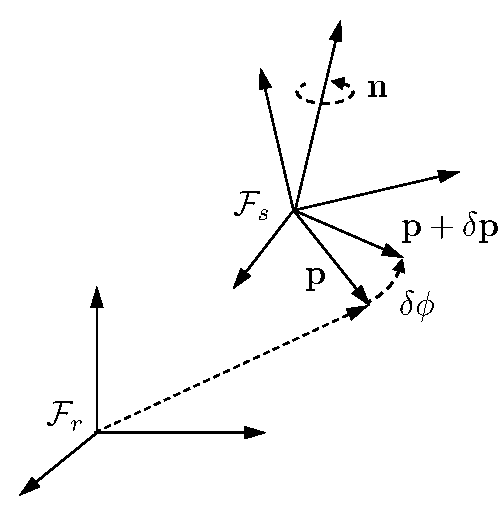
\includegraphics[width=\linewidth]{chap2_preliminaries/figures/coriolis_formula}\\
  \caption{Derivation of the equation of Coriolis.}
  \label{fig:coriolis_formula}
\end{marginfigure}
On the other hand, assume that $\mathbf{p}$ is fixed in
$\mathcal{F}_s$ but that $\mathcal{F}_s$ is rotating with respect to
$\mathcal{F}_r$, and let $\omegabf_{s/r}$ be the instantaneous axis of
rotation and $\delta\phi$ the (right-handed) rotation angle.  Then
the Rodrigues formula~\eqref{eq:rodrigues_1} gives
\begin{align*}
\mathbf{p}+\delta\mathbf{p} 
	&=\Big[I + \sin(\delta\phi)\ss{\nbf} + (1-\cos(\delta\phi))\ss{\nbf}^2\Big]\pbf \\
	&\approx \Big[I + \delta\phi \ss{\nbf} + (\delta\phi^2)\ss{\nbf}^2\Big]\pbf \\
	&\approx \Big[I + \delta\phi \ss{\nbf}\Big]\pbf \\
	&= \pbf + (\delta\phi\nbf)\times \pbf,
\end{align*}
which implies, after dividing both sides by $\delta t$ that
\[
\frac{\delta\mathbf{p}}{\delta t} \approx \frac{\delta\phi}{\delta
t}\nbf \times \mathbf{p}.
\]
Taking the limit as $\delta t \to 0$ and defining the angular
velocity of $\mathcal{F}_s$ with respect to $\mathcal{F}_r$ as
$\boldsymbol{\omega}_{s/r}
\defeq \dot{\phi}\nbf$ we get
\begin{equation}\label{eq:coriolis2}
\frac{d\mathbf{p}}{dt_r} = \omegabf_{s/r}\times\mathbf{p}.
\end{equation}
Since differentiation is a linear operator we can combine
Equations~\eqref{eq:coriolis1}
and~\eqref{eq:coriolis2} to obtain
\begin{equation}\label{eq:coriolis}
\frac{d\mathbf{p}}{dt_r} = \frac{d\mathbf{p}}{dt_s} + \boldsymbol{\omega}_{s/r}
\times\mathbf{p},
\end{equation}
which is the equation of Coriolis.

Note that the vectors in Equation~\eqref{eq:coriolis} have not yet been expressed with respect to a particular coordinate system.  In fact, we can express each vector in Equation~\eqref{eq:coriolis} with respect to any given coordinate frame.  However, care needs to be taken to express the vectors {\bf after} the differentiation operator. For example, expressing the equations in frame $\cal{F}_s$ we have 
\[
\left(\frac{d\mathbf{p}}{dt_r}\right)^s = \left(\frac{d\mathbf{p}}{dt_s}\right)^s + \omegabf_{s/r}^s \times \mathbf{p}^s.
\]
Note however that $\left(\frac{d\mathbf{p}}{dt_r}\right)^s$ is not necessarily equal to $\frac{d\left(\mathbf{p}^s\right)}{dt_r}$.  For example, suppose that $\ibf_s$ is the unit vector along the $x$-axis of the $s$-frame that is undergoing a pure rotation denoted by $\boldsymbol{\omega}_{s/r}$.  Then it is clear that $\left(\frac{d\ibf_s}{dt_r}\right)^s = \omegabf_{s/r}^s\times\ibf_s^s \neq 0$.  However, since $\ibf_s^s = (1, 0, 0)^\top$ is constant in the $s$-frame, $\frac{d\left(\ibf_s^s\right)}{dt_r}=0$.  
%
It is true however that $\left(\frac{d\mathbf{p}}{dt_s}\right)^s =  \frac{d\left(\mathbf{p}^s\right)}{dt_s}$. In general, if the time derivative of the vector is with respect to the same frame in which the vector is being expressed, then the derivative of the vector with respect to frame $s$ expressed in frame $s$ is equal to the derivative of the vector expressed in frame $s$ with respect to frame $s$. 


We also note that the derivative of a scalar is independent of the coordinate frame with which the derivative is being taken.  In this book we will use the dot-notation to mean differentiation with respect to time, only when the derivative is applied component wise, and each component is being differentiated as a scalar.  In that sense, if $\mathbf{p}^s = (x, y, z)^{\top}$, then 
\[
\frac{d\mathbf{p}^s}{dt_s} = \begin{pmatrix} \dot{x} \\ \dot{y} \\ \dot{z} \end{pmatrix}.
\]
When vectors are expressed relative to a coordinate frame, then Equation~\eqref{eq:coriolis} can be written as
\[
\left(\frac{d\mathbf{p}}{dt_r}\right)^q = \left(\frac{d\mathbf{p}}{dt_s}\right)^q+ \ss{\omegabf_{s/r}^q}\mathbf{p}^q.
\]

%%+++++++++++++++++++
\subsection{Rotational Kinematics} 

The Coriolis equation~\eqref{eq:coriolis}
facilitates the derivation of the rotational kinematics of a rigid body.  Defining coordinate frame $s$ as $\mathcal{F}_s = \{\ibf_s, \jbf_s, \kbf_s\}$,
and suppose that frame $s$ is rotated relative to frame $r$ by angular velocity $\omegabf_{s/r}$, then the Coriolis formula gives
\[
\frac{d\ibf_s}{dt_r} = \frac{d\ibf_s}{dt_s} + \omegabf_{s/r}\times\ibf_s, \qquad 
\frac{d\jbf_s}{dt_r} = \frac{d\jbf_s}{dt_s} + \omegabf_{s/r}\times\jbf_s, \qquad 
\frac{d\kbf_s}{dt_r} = \frac{d\kbf_s}{dt_s} + \omegabf_{s/r}\times\kbf_s.
\]
Since the coordinate axes are stationary in their own frame, $\frac{d\ibf_s}{dt_s}=\frac{d\jbf_s}{dt_s}=\frac{d\kbf_s}{dt_s}=0$, and we have
\[
\frac{d\ibf_s}{dt_r} = \omegabf_{s/r}\times\ibf_s, \qquad 
\frac{d\jbf_s}{dt_r} = \omegabf_{s/r}\times\jbf_s, \qquad 
\frac{d\kbf_s}{dt_r} = \omegabf_{s/r}\times\kbf_s.
\]
Expressing all vectors in frame $r$ and rewriting in matrix notation gives
\begin{align*}
\begin{bmatrix} \frac{d\ibf_s^r}{dt_r} & \frac{d\jbf_s^r}{dt_r} & \frac{d\kbf_s^r}{dt_r} \end{bmatrix} 
&= \begin{bmatrix} \ss{\omegabf_{s/r}^r}\ibf_s^r, & \ss{\omegabf_{s/r}^r}\jbf_s^r, & \ss{\omegabf_{s/r}^r}\kbf_s^r, \end{bmatrix}  \\
&= \ss{\omegabf_{s/r}^r} \begin{bmatrix} \ibf_s^r & \jbf_s^r & \kbf_s^r \end{bmatrix}  \\
&= \ss{\omegabf_{s/r}^r} R_s^r. 
\end{align*}
Defining 
\[
\dot{R}_s^r \defeq \begin{bmatrix} \frac{d\ibf_s^r}{dt_r} & \frac{d\jbf_s^r}{dt_r} & \frac{d\kbf_s^r}{dt_r} \end{bmatrix}
\]
gives the rotational kinematics as
\begin{equation}\label{eq:rotational_kinematics_1}
\dot{R}_s^r = \ss{\omegabf_{s/r}^r} R_s^r.
\end{equation}

Suppose that we equate the $s$-frame with the body frame $\mathcal{F}_b$ and the $r$-frame with the inertial frame $\mathcal{F}_i$, then Equation~\eqref{eq:rotational_kinematics_1} becomes
\[
\dot{R}_b^i = \ss{\omegabf_{b/i}^i} R_b^i,
\]
which is given in terms of the angular velocity $\omegabf_{b/i}$ expressed in the inertial frame.  However, the angular velocity can be measured with respect to the body frame using rate gyros.  Therefore, it is preferable to write the rotational kinematics in terms of $\omegabf_{b/i}^b$.  Noting that $\omegabf_{s/r}^r = R_s^r \omegabf_{s/r}^s$, we get
\marginnote{Note that we have used Equation~\eqref{eq:skew_matrix_6} $\ss{(R\nbf)}=R\ss{\nbf}R^\top$.}
\begin{align*}
\dot{R}_s^r &= \ss{\omegabf_{s/r}^r} R_s^r	\\
			&= \ss{R_s^r\omegabf_{s/r}^s} R_s^r \\
			&= R_s^r \ss{\omegabf_{s/r}^s} (R_s^r)^\top R_s^r \\
			&= R_s^r \ss{\omegabf_{s/r}^s}.
\end{align*}
We have therefore established the relationship for rotational kinematics as
\begin{align}
	\dot{R}_s^r &= R_s^r \ss{\omegabf_{s/r}^s} \label{eq:rotational_kinematics} \\
				&= \ss{\omegabf_{s/r}^r} R_s^r \label{eq:rotational_kinematics_alt}
\end{align}

Applying these formulas to the body and inertial frames we have
\begin{align}
\dot{R}_b^i &= R_b^i \ss{\omegabf_{b/i}^b} = \ss{\omegabf_{b/i}^i} R_b^i \label{eq:rotational_kinematics_b_i} \\
\dot{R}_i^b &= -\ss{\omegabf_{b/i}^b} R_i^b = - R_i^b \ss{\omega_{b/i}^i}.\label{eq:rotational_kinematics_i_b}
\end{align}
Applying these formulas to the gimbal and body frames we have
\begin{align*}
\dot{R}_g^b &= R_g^b \ss{\omegabf_{g/b}^g} = \ss{\omegabf_{g/b}^b} R_g^b \\
\dot{R}_b^g &= -\ss{\omegabf_{g/b}^g} R_b^g = - R_b^g \ss{\omega_{g/b}^b}.
\end{align*}

Using the conclusions of the previous section, we can get the following result.
\begin{lemma}
If $\mathbf{p}$ is a vector and $\mathcal{F}^s$ and $\mathcal{F}^r$ are coordinate frames, with $R_r^s\in SO(3)$ being the rotation between frames, then
\[
\left(\frac{d\mathbf{p}}{dt_r}\right)^s = R_r^s\frac{d (\mathbf{p}^r)}{dt_s}.
\]	
\end{lemma}
\begin{proof}
	\begin{align*}
			\left(\frac{d\mathbf{p}}{dt_r}\right)^s 
				&= \left(\frac{d\mathbf{p}}{dt_s}\right)^s + \omegabf_{s/r}^s \times \mathbf{p}^s \\
				&= \frac{d(\mathbf{p}^s)}{dt_s} + \ss{\omegabf_{s/r}^s} R_r^s \mathbf{p}^r \\
				&= \frac{d(R_r^s\mathbf{p}^r)}{dt_s} + \ss{\omegabf_{s/r}^s} R_r^s \mathbf{p}^r \\
				&= \frac{dR_r^s}{dt_s}\mathbf{p}^r + R_r^s \frac{d(\mathbf{p}^r)}{dt_s} +\ss{\omegabf_{s/r}^s} R_r^s \mathbf{p}^r \\
				&= -\ss{\omegabf_{s/r}^s} R_r^s\mathbf{p}^r + R_r^s \frac{d(\mathbf{p}^r)}{dt_s} +\ss{\omegabf_{s/r}^s} R_r^s \mathbf{p}^r \\
				&= R_r^s \frac{d(\mathbf{p}^r)}{dt_s}.
	\end{align*}
\end{proof}




%%+++++++++++++++++++
\subsection{Integrating the Rotational Kinematics}
In robotics and flying vehicle applications, we often need to integrate the rotational kinematics given samples of the rate gyros. 
In this section we describe numerical approximations to the equation
\begin{equation}\label{eq:Rdot-integrating-1}
\dot{R}=R\ss{\omegabf},
\end{equation}
assuming that $\omegabf$ is either piecewise constant, or piecewise linear between samples.  Since $R$ evolves on the set $SO(3)$, the simple Euler integration scheme $R[k]=R[k-1]+TR[k-1]\ss{\omegabf[k]}$ is particularly bad since $R$ immediately leaves $SO(3)$.  A common strategy is to re-orthonormalize $R$ after every integration step, but this is an ad~hoc scheme that may introduce additional drift in the integration process.  If $\omegabf$ is assumed to be piecewise constant or piecewise linear between samples, then the kinematics can be integrated exactly.  

We begin by solving the differential equation~\eqref{eq:Rdot-integrating-1}.
\begin{lemma} \label{eq:rotation_kinematics_solution}
The solution to Equation	~\eqref{eq:Rdot-integrating-1} with initial condition $R(t_0) = R_0$ is given by
\begin{equation}\label{eq:rotation_kinematics_solution}
R(t) = R(t_0)\exp\left(\ss{\int_{t_0}^t \omegabf(\tau) d\tau }\right).
\end{equation}
\end{lemma}
\begin{proof}
Rewrite Equation~\eqref{eq:Rdot-integrating-1} as
\[
\dot{R} - R\ss{\omegabf} = 0,
\]
and multiply on the left by the integrating factor $\exp\left(-\ss{\int_{t_0}^t\omegabf(\tau)d\tau}\right)$ to get
\begin{align*}
\left(\dot{R} - R\ss{\omegabf}\right)\exp\left(-\ss{\int_{t_0}^t \omegabf(\tau)d\tau}\right) &=\\
\frac{d}{dt}\left[R\exp\left(-\ss{\int_{t_0}^t \omegabf(\tau)d\tau}\right)\right] &= 0.
\end{align*}
Integrating both sides and applying the fundamental theorem of Calculus gives 
\marginnote{The fundamental theorem of Calculus states that $\int_a^b dF = F(b)-F(a)$.}
\begin{equation}\label{eq:rotation_kinematics_solution}
R(t)\exp\left(\ss{-\int_{t_0}^t \omegabf(\tau) d\tau} \right) - R(t_0)\exp\left(\ss{-\int_{t_0}^{t_0} \omegabf(\tau) d\tau} \right) = 0.
\end{equation}
\marginnote{In deriving this expression, we have used the fact that $\exp(-Mt)=(\exp(Mt))^{-1}$ and $\exp(Mt)\exp(-Mt_0)=\exp(M(t-t_0))$.}
Multiplying on the left by $\exp\left(\ss{\int_{t_0}^t \omegabf(\tau) d\tau }\right)$ gives the result.
\end{proof}

In the following, we let $T_s$ represent the sample rate, and we will use the notation $R[k]=R(kT_s)$ and $\omegabf[k]\defeq\omegabf(kT_s)$.  We say that $\omegabf$ is piecewise constant between samples if
\[
\omegabf(t) = \omegabf[k]
\]
for $(k-1)T_s < t \leq kT_s$, and we say that $\omegabf$ is piecewise linear between samples if
When $\omegabf$ is piecewise linear between samples, i.e., when
\[
 \omegabf(t) = \left(\frac{kT_s-t}{T_s}\right)\omegabf[k-1] + \left(\frac{(t-(k-1)T_s)}{T_s}\right)\omegabf[k]
\]
for $(k-1)T_s \leq t < kT_s$.
\begin{lemma}
 If the angular velocity is piecewise constant between samples, then from Equation~\eqref{eq:rotation_kinematics_solution} we get
\begin{equation}\label{eq:rotational_int_constant_omega}
R[k] = R[k-1] \exp\left(T_s \ss{\omegabf[k]} \right).
\end{equation}
Similarly, if the angular velocity is piecewise linear between samples, then 
\begin{equation}\label{eq:rotational_int_linear_omega}
R[k] = R[k-1] \exp\left(\frac{T_s}{2} \ss{\omegabf[k]+\omegabf[k-1]}\right).
\end{equation}
\end{lemma}
\begin{proof}
If the sample rate is $T_s$, then letting $t=kT_s$ and $t_0=(k-1)T_s$, and using the notation $R[k]=R(kT)$, we get
\[
R[k] = R[k-1] \exp\left(\ss{\int_{(k-1)T_s}^{kT_s} \omegabf(\tau) d\tau }\right).
\]
When $\omegabf$ is piecewise constant between samples we have
\[
\int_{(k-1)T_s}^{kT_s} \omegabf(\tau) d\tau = \omegabf[k]T_s,
\]
resulting in Equation~\eqref{eq:rotational_int_constant_omega}.
When $\omegabf$ is piecewise linear between samples we get 
\begin{align*}
\int_{(k-1)T_s}^{kT_s} \omegabf(\tau) d\tau
	&= \int_{(k-1)T_s}^{kT_s} \left[\left(\frac{kT_s-\tau}{T_s}\right)\omegabf[k-1] + \left(\frac{\tau-(k-1)T_s}{T_s}\right)\omegabf[k]\right] d\tau \\
	&= \frac{T_s}{2} \left(\omegabf[k]+\omegabf[k-1]\right),
\end{align*}
resulting in Equation~\eqref{eq:rotational_int_linear_omega}.
\end{proof}

%%+++++++++++++++++++
\subsection{Numerical Differentiation of the Rotation Matrix}
\label{sec:numerical_differentiation_of_R}
Similarly, if we are given samples of $R(t)$ at sample rate $T_s$, we would like to approximate the angular velocity $\omegabf(t)$.   
\begin{lemma}
Given the rotational kinematics in Equation~\eqref{eq:Rdot-integrating-1}, and measured rotation matrices $R[k]$ and $R[k-1]$, then
\begin{equation}\label{eq:rotational_diff}
\omegabf[k]\approx \left[\frac{1}{T_s}\log\left(R^\top[k-1]R[k]\right)\right]^{\vee}.
\end{equation}
\end{lemma}
\begin{proof}
From Equation~\eqref{eq:rotational_int_constant_omega} we have
\[
R[k] = R[k-1]\exp\left(T_s\ss{\omegabf[k]}\right).
\]
Solving for $\ss{\omegabf[k]}$ gives
\[
\ss{\omegabf[k]} = \frac{1}{T_s}\log\left(R^\top[k-1]R[k]\right)
\]
from which we obtain Equation~\eqref{eq:rotational_diff}.
\end{proof}



%++++++++++++++++++++++++++++++++++++++++++++++++++++++++++++++++
\subsection{Quaternion Kinematics}
\rwbcomment{Add this later.}

%++++++++++++++++++++++++++++++++++++++++++++++++++++++++++++++++
\subsection{Euler Angle Kinematics}
\rwbcomment{Add this later.}

%++++++++++++++++++++++++++++++++++++++++++++++++++++++++++++++++
\subsection{Rotation Vector Kinematics}
\rwbcomment{Add this later.}

%-----------------------------------------------------------
\section{Homogeneous Transformations}
\label{sec:homogeneous transformations}

In this section we discuss the use of homogeneous transformations to represent rigid body motion that includes both translation and rotation simultaneously.  We will show that $4\times 4$ matrices can be used to represent rigid body motion.
%
\begin{marginfigure}[-2in]
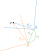
\includegraphics[width=\linewidth]{chap2_preliminaries/figures/transform_passive}
\caption{Illustration of a passive transformation}
\label{fig:passive_transform}
\end{marginfigure}
Considering Figure~\ref{fig:passive_transform}, 
suppose that a robot moves from a pose represented by frame $\mathcal{F}_a$ to a pose represented by frame $\mathcal{F}_b$.  If the robot measures the position of point $\pbf$ in frame $a$ and from odometry knows its relative motion represented by the rotation matrix $R_a^b$ and the translation vector $\tbf_{a/b}^b$, then the position of $\pbf$ relative to frame $\mathcal{F}_b$ is given by
\begin{equation}\label{eq:homogenenous_1}
\rbf_{p/b}^b = R_a^b \rbf_{p/a}^a + \tbf_{a/b}^b.
\end{equation}
We would like to represent this relative motion using a matrix.  
%
To do so, we introduce the use of {\em homogeneous coordinates} for position.  The homogeneous coordinates of the vector $\pbf^c$ expressed in a general frame $\mathcal{F}_c$ are given by
\[
\bar{\pbf}^c \defeq \begin{pmatrix} \pbf^c \\ 1 \end{pmatrix},
\]
where $1$ has been appended as the last coordinate.  
%
Using this notation, Equation~\eqref{eq:homogenenous_1} can be written as
\[
\bar{\rbf}_{p/b}^b = \begin{pmatrix} \rbf_{p/b}^b \\ 1 \end{pmatrix} = \begin{pmatrix} R_a^b & \tbf_{a/b}^b \\ 0 & 1 \end{pmatrix}\begin{pmatrix} \rbf_{p/a}^a \\ 1 \end{pmatrix} = T_a^b \bar{\rbf}_{p/a}^a,
\]
where
\[
T_a^b \defeq \begin{pmatrix} R_a^b & \tbf_{a/b}^b \\ 0 & 1 \end{pmatrix}
\]
is called a homogeneous transformation matrix.
%
It is important to note is that the translation
vector is defined in the \emph{destination} frame, rather than the
origin frame of the rotation matrix. 

%
%
%
%
%Now we venture into the world of rigid body transformations. These
%allow us to represent both translation and rotation simultaneously.
%As with rotations, there are two popular representations that I will
%consider in this document, the first is matrix-based, the set of $4\times4$
%matrices, commonly known as $SE(3)$. The second (like
%rotations) will be based on complex numbers, dual unit quaternions.
%There are actually other representations, but we will see later all
%of these groups share the same Lie Algebra! Therefore, we can choose
%the representation that we feel most comfortable with, or is the most
%efficient, etc... It really doesn't matter, which is a great thing.

\subsection{Homogeneous Transformation Matrices}

Define the set
\[
SE(3) = \left\{T\in\mathbb{R}^{4\times 4} ~|~ T=\begin{pmatrix} R & \tbf \\ 0 & 1\end{pmatrix}, R\in SO(3), \tbf\in\mathbb{R}^3 \right\},
\]
which is called the {\em Special Euclidean group of dimension 3}.  We can derive the following facts about elements of $SE(3)$.

\begin{lemma}[Closed under Multiplication]
If $T_1, T_2\in SE(3)$, then $T_3=T_2 T_1 \in SE(3)$.
\end{lemma}
\begin{proof}
	\begin{align*}
	T_3 &= \begin{pmatrix} R_2 & \tbf_2 \\ 0 & 1 \end{pmatrix} \begin{pmatrix} R_1 & \tbf_1 \\ 0 & 1 \end{pmatrix} \\
	    &= \begin{pmatrix} R_2 R_1 & R_2\tbf_1 + \tbf_2 \\ 0 & 1 \end{pmatrix},
	\end{align*}
	which is an element of $SE(3)$ since $SO(3)$ is closed under multiplication and $R_2\tbf_1 + \tbf_2\in\mathbb{R}^3$.
\end{proof}

\begin{lemma}[Inverse]
If 
\[
T=\begin{pmatrix} R & \tbf \\ 0 & 1\end{pmatrix} \in SE(3),
\]	
then 
\[
T^{-1} =\begin{pmatrix} R^\top & -R^\top\tbf \\ 0 & 1\end{pmatrix} \in SE(3).
\]
\end{lemma}
\begin{proof}
The fact that $TT^{-1} = T^{-1}T = I$ can be shown by direct calculation.  Since $R^\top\in S(3)$ when $R\in SO(3)$ and $-R^\top\tbf\in\mathbb{R}^3$ it follows that $T^{-1}\in SE(3)$.
\end{proof}

\begin{lemma} [Determinant]
If $T\in SE(3)$, then $\det(T)=1$.
\end{lemma}
\begin{proof}
Follows from $\det{T}=\det(R)\det(1)=1$.
\end{proof}
\begin{lemma} [Concatination]
If $T_a^b\in SE(3)$ and $T_b^c\in SE(3)$ are homogeneous transformations from frames $a$ to $b$ and $b$ to $c$, respectively, then the homogeneous transformation from frame $a$ to frame $c$ is given by
\begin{align*}
T_{a}^{c} & =T_{b}^{c}\cdot T_{a}^{b}\\
 & =\begin{pmatrix}R_{b}^{c} & \tbf_{c/b}^{c}\\
0 & 1
\end{pmatrix}\cdot\begin{pmatrix}R_{a}^{b} & \tbf_{b/a}^{b}\\
0 & 1
\end{pmatrix}\\
 & =\begin{pmatrix}R_{b}^{c}R_{a}^{b} & R_{b}^{c}\tbf_{b/a}^{b}+\tbf_{c/b}^{c}\\
0 & 1
\end{pmatrix}.
\end{align*}
\end{lemma}

%----------------------------------------
\subsection{Passive and Active Transformations}

The same notion of passive and active transformations discussed with
rotations applies here. To perform a passive transformation with $SE(3)$,
we just pad the vector to be rotated with an extra $1$ at the bottom,
and multiply by the homogeneous transformation matrix. 

\begin{marginfigure}
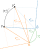
\includegraphics[width=\linewidth]{chap2_preliminaries/figures/transform_active}
\caption{Illustration of an active transformation.}
\label{fig:active_transform}
\end{marginfigure}

An active transformation occurs by multiplying by the inverse of the
passive transform as shown in Figure~\ref{fig:passive_transform}.
Just as with rotations, If you walk through the coordinate frames
of an active transformation, you'll see that the coordinate frames
don't line up right in our notation. This is because the active transformation
does not preserve the location. Instead we have defined a new location,
based on the coordinates of $p$ in frame $a$ projected into frame
$b$. This is represented by the $p^{\star}$ notation
in Figure~\ref{fig:active_transform}.

%Transform matrices are an obvious extension of rotation matrices.
%However, just like rotation matrices, the complex number representation
%is more efficient. This brings us to our next transform parameterization:
%dual unit quaternions.

%++++++++++++++++++++++++++++++++++++++++++++++++++++++++++++++
\subsection{Rigid body kinematics}
As we saw in Section~\ref{sec:rotational_kinematics}, the rotational kinematics are given by
\begin{equation}\label{eq:rotational_dynamics_kinematics}
\dot{R}_s^r = R_s^r \ss{\omegabf_{s/r}^s}.
\end{equation}
In this section we will derive a similar expression for homogeneous transformation matrices.  
Let
\[
T_s^r = \begin{pmatrix} R_s^r & \tbf_{s/r}^r \\ 0 & 1 \end{pmatrix},
\]
and differentiate to get
\begin{align*}
\dot{T}_s^r &= \begin{pmatrix} \dot{R}_s^r & \dot{\tbf}_{s/r}^r \\ 0 & 1 \end{pmatrix} \\
&= \begin{pmatrix} R_s^r\ss{\omegabf_{s/r}^s} & R_s^r\dot{\tbf}_{s/r}^s \\ 0 & 1 \end{pmatrix} \\
&= \begin{pmatrix} R_s^r & \tbf_{s/r}^r \\ 0 & 1 \end{pmatrix} \begin{pmatrix} \ss{\omegabf_{s/r}^s} & \dot{\tbf}_{s/r}^s \\ 0 & 0 \end{pmatrix}
\end{align*}
Define the relative velocity as
\[
\vbf_{s/r} \defeq \dot{\tbf}_{s/r},
\]
and the relative twist as
\[
\nubf_{s/r} = \begin{pmatrix} \vbf_{s/r} \\ \omegabf_{s/r} \end{pmatrix}.
\]
We also define the ``wedge'' operator for twist as 
\[
\begin{pmatrix} \vbf_{s/r} \\ \omegabf_{s/r} \end{pmatrix}^\wedge = \begin{pmatrix} \ss{\omegabf_{s/r}} & \vbf_{s/r} \\ 0 & 0 \end{pmatrix},
\]
and we define $\se(3)$ to be the set of all ``wedged'' twist vectors:
\[
\se(3) = \left\{ \Omega = \begin{pmatrix}\ss{\omegabf} & \nubf \\ 0 & 0\end{pmatrix} ~|~ \nubf, \omegabf \in \mathbb{R}^3 \right\}.
\] 

We have that the homogeneous transformation matrix evolves as
\begin{equation}\label{eq:homogeneous_diffeq}
\dot{T}_s^r = T_s^r (\nubf_{s/r}^s)^\wedge,
\end{equation}
where $T_s^r\in SO(3)$ and $(\nubf_{s/r}^s)^\wedge\in\se(3)$, 
which has the same form as Equation~\eqref{eq:rotational_dynamics_kinematics}.  Analogous to Equations~\eqref{eq:rotational_kinematics_b_i} and~\eqref{eq:rotational_kinematics_i_b}, the kinematics of the multirotor body frame relative to the inertial frame are given by
\begin{align}
\dot{T}_b^i &= T_b^i (\nubf_{b/i}^b)^\wedge = (\nubf_{b/i}^i)^\wedge T_b^i \label{eq:homogeneous_kinematics_b_i} \\
\dot{T}_i^b &= -(\nubf_{b/i}^b)^\wedge T_i^b = - T_i^b (\nubf_{b/i}^i)^\wedge.\label{eq:homogeneous_kinematics_i_b}
\end{align}

The following lemma provide a solution to the differential equation~\eqref{eq:homogeneous_diffeq}.
\begin{lemma}
The solution to differential matrix equation
\[
\dot{T} = T\nubf^\wedge
\]
with initial condition $T(t_0)$ is given by
\begin{equation}\label{eq:homogeneous_kinematics_solution}
T(t) = T(t_0)\exp\left(\int_{t_0}^t \nubf(\tau) d\tau \right)^\wedge.
\end{equation}
\end{lemma}
\begin{proof}
Similar to Lemma~\ref{eq:rotation_kinematics_solution}.	
\end{proof}

We now derive an expression for the exponential of a matrix $\Omega\in\se(3)$.
\begin{lemma}
If $\nubf^\wedge = \begin{pmatrix} \ss{\omegabf} & \vbf \\ 0 & 0 \end{pmatrix} \in \se(3)$, then
\[
\exp(\nubf^\wedge) = \begin{pmatrix} \exp(\ss{\omegabf}) & W(\ss{\omegabf})\vbf \\ 0 & 1 \end{pmatrix},
\]
where
\[
W(\ss{\omegabf}) \defeq I+\left(\frac{1-\cos\left(\norm{\omegabf}\right)}{\norm{\omegabf}^{2}}\right)\ss{\omegabf}+\left(\frac{\norm{\omegabf}-\sin\left(\norm{\omegabf}\right)}{\norm{\omegabf}^{3}}\right)(\ss{\omegabf})^{2}.
\]
Furthermore $\exp(\nubf^\wedge) \in SE(3)$.
\end{lemma}
\begin{proof}
\begin{align*}
\exp\begin{pmatrix}\ss{\omegabf} & \vbf\\
0 & 0
\end{pmatrix} & =I+\begin{pmatrix}\ss{\omegabf} & \vbf\\
0 & 0
\end{pmatrix}+\frac{1}{2!}\begin{pmatrix}\ss{\omegabf} & \vbf\\
0 & 0
\end{pmatrix}^{2}+\frac{1}{3!}\begin{pmatrix}\ss{\omegabf} & \vbf\\
0 & 0
\end{pmatrix}^{3}+\cdots\\
 & =I+\begin{pmatrix}\ss{\omegabf} & \vbf\\
0 & 0
\end{pmatrix}+\frac{1}{2!}\begin{pmatrix}(\ss{\omegabf})^{2} & \ss{\omegabf}\vbf\\
0 & 0
\end{pmatrix}+\frac{1}{3!}\begin{pmatrix}(\ss{\omegabf})^{3} & (\ss{\omegabf})^{2}\vbf\\
0 & 0
\end{pmatrix}+\cdots\\
 & =\begin{pmatrix}\exp\left(\ss{\omegabf}\right) & W(\ss{\omegabf}) \vbf\\
0 & 0
\end{pmatrix},
\end{align*}
where
\begin{align*}
W(\ss{\omegabf}) &= I+\frac{1}{2}\ss{\omegabf}+\frac{1}{3!}(\ss{\omegabf})^{2} + \ddots \\
	&= I + \sum_{k=0}^{\infty}\left(\frac{(\ss{\omegabf})^{\left(2k+1\right)}}{\left(2k+2\right)!}+\frac{(\ss{\omegabf})^{\left(2k+2\right)}}{\left(2k+3\right)!}\right).
\end{align*}
Recall from the proof of Lemma~\ref{lem:rodrigues_exponential} that 
\begin{align*}	
\ss{\nbf}^{(2m+1)} &= (-1)^m\ss{\nbf} \\
\ss{\nbf}^{(2m+2)} &= (-1)^m\ss{\nbf}^2,
\end{align*}
from which we get
\begin{align*}
W(\ss{\omegabf}) 
 & =I+\sum_{k=0}^{\infty}\left(\frac{\left(-1\right)^{k}\norm{\omegabf}^{2k}}{\left(2k+2\right)!}\right)\ss{\omegabf}+\sum_{k=0}^{\infty}\left(\frac{\left(-1\right)^{k}\norm{\omegabf}^{2k}}{\left(2k+3\right)!}\right)(\ss{\omegabf})^{2}\\
 & =I+\left(\frac{1}{2}-\frac{\norm{\omegabf}^{2}}{4!}+\frac{\norm{\omegabf}^{4}}{6!}+\cdots\right)\ss{\omegabf}+\left(\frac{1}{3!}-\frac{\norm{\omegabf}^{2}}{5!}+\frac{\norm{\omegabf}^{4}}{7!}+\cdots\right)(\ss{\omegabf})^{2}\\
 & =I+\left(\frac{1-\cos\left(\norm{\omegabf}\right)}{\norm{\omegabf}^{2}}\right)\ss{\omegabf}+\left(\frac{\norm{\omegabf}-\sin\left(\norm{\omegabf}\right)}{\norm{\omegabf}^{3}}\right)(\ss{\omegabf})^{2}.
\end{align*}
The fact that $\exp(\Omega)\in SE(3)$ follows from the definition of $SE(3)$ since $\exp(\ss{\omegabf})\in SO(3)$ and $W(\ss{\omegabf})\vbf\in\mathbb{R}^3.$
\end{proof}
The logarithm also has a closed form.
\begin{lemma}
If $R\in SO(3)$ and $\tbf\in\mathbb{R}^3$, then
\[
\log\begin{pmatrix} R & \tbf \\ 0 & 1 \end{pmatrix} = \begin{pmatrix}\log(R) & W^{-1}\tbf \\ 0 & 0 \end{pmatrix},
\]
where
\[
W^{-1}(R) = I - \frac{1}{2}\ss{\omegabf} + \frac{1}{\theta^2}\left(1-\frac{\theta\sin\theta}{2(1-\cos\theta)}\right)\ss{\omegabf}^2,
\]
where $\omegabf = \log(R)^\vee$ and $\theta=\norm{\omegabf}$.
\end{lemma}
\begin{proof}
From the previous lemma we know that
\[
\log\begin{pmatrix} \exp(\ss{\omegabf}) & W\vbf \\ 0 & 1 \end{pmatrix} 
= \begin{pmatrix} \ss{\omegabf} & \vbf \\ 0 & 0 \end{pmatrix}.
\]
Equation $R=\exp(\ss{\nubf^\wedge})$ and $\tbf = W\vbf$ shows that $\omegabf=\log(R)^\vee$ and $\vbf=W^{-1}\tbf$.
	
\end{proof}






%%++++++++++++++++++++++++++++++++++++++++++++++++++++++++++++++++
%\subsection{Body-Centric vs Inertial Representation}
%
%In robotics or computer vision, we are typically concerned with rotations
%so that we can describe the movement of physical objects. When we
%do this, it turns out that choice of coordinate frame also introduces
%some interesting consequences that may or may not be intentional.
%Rotational dynamics of any arbitrary coordinate frame $j$ with respect
%to another coordinate frame $i$ is given by
%
%\[
%\dot{R}_{i}^{j}=R_{i}^{j}\ss{(\omegabf_{i/j}^{i})}.
%\]
%However, let's study a concrete example: the dynamics of some rigid
%body undergoing pure rotation. If we define some inertial frame $I$
%and the moving, body frame as $b$, then the dynamics of the \emph{body-centric}
%rotation matrix (i.e. body$\to$inertial), we get 
%
%\begin{equation}
%\dot{R}_{b}^{I}=R_{b}^{I}\ss{(\omegabf_{b/I}^{b})},\label{eq:body_rot_dyn}
%\end{equation}
%and the \emph{inertial} rotation matrix is (inertial$\to$body) evolves
%according to
%
%\begin{equation}
%\dot{R}_{I}^{b}=R_{I}^{b}\ss{(\omegabf_{I/b}^{I})}.\label{eq:inertial_rotation_dynamics}
%\end{equation}
%This is all fine, except that we typically measure angular velocity
%in the body coordinate frame $\omegabf_{b/I}^{b}.$ Therefore, it is much
%more convenient to express Eq. \ref{eq:inertial_rotation_dynamics}
%in terms of body angular rates. If we do this, then we get
%
%\begin{align*}
%\dot{R}_{I}^{b} & =R_{I}^{b}\ss{(-R_{b}^{I}\omegabf_{b/I}^{b})} & \text{(Negate and rotate $\omegabf$)}\\
% & =-\ss{(\omegabf_{b/I}^{b})}R_{I}^{b}, & \text{(Eq. \ref{eq:skew_trick_2})}
%\end{align*}
%which can also be easily derived as the transpose of Eq \ref{eq:body_rot_dyn}.
%The desire to express our angular rates in terms of the body frame
%induces a similar effect in unit quaternion dynamics, except that
%it is reversed due to the reversed order of concatenation:
%
%\begin{align}
%\dot{\qbf}_{I}^{b} & =\frac{1}{2}\qbf_{I}^{b}\cdot\begin{pmatrix}0\\
%\omegabf_{b/I}^{b}
%\end{pmatrix}\label{eq:quaternion_dynamics}\\
%\dot{\qbf}_{b}^{I} & =-\frac{1}{2}\begin{pmatrix}0\\
%\omegabf_{b/I}^{b}
%\end{pmatrix}\cdot\qbf_{b}^{I}.\nonumber 
%\end{align}
%
%Any advantage to expressing attitude in body-centric vs. inertial
%coordinates will be use-case specific, so both representations are
%used widely in literature. Because both representations are often
%used, however, it can sometimes be confusing to compare two works
%which may be expressing their attitude differently, especially if
%neither work is specific about their representation.


%\subsection{The Solution to the Rotational Dynamics Equation}
%
%Equations \ref{eq:body_rot_dyn} and \ref{eq:inertial_rotation_dynamics}
%are first-order matrix differential equations. These are solved with
%the matrix exponential we discussed in Section \ref{sec:mat_exp}.
%The solution to the body-centric equation is
%
%\[
%R_{b}^{I}\left(t\right)=R_{b}^{I}\left(t_{0}\right)\exp\left(\ss{(\omegabf_{b/I}^{b})}t\right)
%\]
%and the inertial dynamics are solved with
%
%\[
%R_{I}^{b}\left(t\right)=\exp\left(-\ss{(\omegabf_{b/I}^{b})}t\right)R_{I}^{b}\left(t_{0}\right).
%\]
%Quaternion dynamics are also easily solved in a similar fashion, as
%in
%
%\begin{align*}
%\qbf_{b}^{I}\left(t\right) & =\exp\begin{pmatrix}0\\
%-\omegabf_{b/I}^{b}t
%\end{pmatrix}\cdot\qbf_{b}^{I}\left(t_{0}\right)\\
%\qbf_{I}^{b}\left(t\right) & =\qbf_{I}^{b}\left(t_{0}\right)\cdot\exp\begin{pmatrix}0\\
%\omegabf_{b/I}^{b}t
%\end{pmatrix}.
%\end{align*}
%The infinite series Eq. \ref{eq:mat_exp_inf} can be used to compute
%these directly. However, efficient closed-form implementations are
%derived in Section \ref{sec:matrix_exp_closed_form}.

%---------------------------------------------
\section{Lie Groups}

Lie Group theory is a very old discipline deeply rooted in mathematics
and theoretical physics. It was developed to better understand and
model nature at the most fundamental levels. In fact, much of particle
physics can be modeled using Lie group theory, including special relativity
and quantum dynamics. 

Robotics requires us to reason about different coordinate frames. We often need to
reason about how they move, and how they relate to one another. We
also find ourselves trying to infer things about these coordinate
frames given noisy sensor measurements. There are a variety of ways
that we could do this, but the real problems show up when we need
to this in real time under realistic computational limitations. 

To meet actual computational requirements, we generally want to be
able to leverage linear algebra and all of its tools. Unfortunately,
however, coordinate frame transformations are not vectors, so it's
not completely obvious how we can use these tools in a principled
manner. Luckily, we have Lie group theory that can bridge this gap.
We will see in this section how we can use Lie Groups to take non-vector
group objects, and map them into a vector space where we can perform
linear algebra and reason about things in an efficient manner, then
map our results back into the group so we can do useful things.

As a further motivating example, consider the case where we might
want to represent the uncertainty of the estimate of a rotation matrix.
In general, assuming that the uncertainty of some vector quantity
$\xbf$ can be represented with a multivariate Gaussian distribution where
the covariance of the distribution is computed as
\[
\Sigma_{\xbf}=E\left[\left(\xbf-\hat{\xbf}\right)\left(\xbf-\hat{\xbf}\right)^{\top}\right],
\]
where $\hat{\xbf}$ is the mean of the distribution and $\xbf$ is the true value.
However, this equation does not work for rotation matrices in part because $R-\hat{R}$ is not meaningful because subtraction is not a sensible
operation for rotation matrices. In addition, $R$ has nine parameters but only three degrees of freedom, and so we expect the uncertainty covariance to be $3\times 3$.  \marginnote{Euler angles do not solve the problem, because subtracting two ``vectors'' of Euler angles is problematic if the angles are larger than 180 degrees.}. Lie group theory addresses this problem in a very satisfactory way.

%+++++++++++++++++++++++++++++++++++++++++++++++++++++++++
\subsection{Group Theory}

Before we launch into Lie groups, lets consider groups generically.
A group is a set of objects $\mathcal{G}$ together with an operation 
\[
\circ: \mathcal{G} \times \mathcal{G} \to \mathcal{G},
\]
with the following properties:
\begin{description}
\item[G.1] The groups is closed under $\circ$, meaning that if $G_1, G_2\in\mathcal{G}$, then $G_1\circ G_2\in \mathcal{G}$.
\item[G.2] There exists an identity element $E\in\mathcal{G}$ so that for any other $G\in\mathcal{G}$, $E\circ G = G\circ E = G$.
\item[G.3] For every $G\in\mathcal{G}$, there exists a $G^{-1}\in\mathcal{G}$ such that $G\circ G^{-1}=G^{-1}\circ G = E$.	
\end{description}

We use groups all the time, maybe without knowing it. Some commonly
used groups in robotics are vectors (closed under vector addition),
rotation matrices (closed under matrix multiplication), and quaternions
(closed under quaternion multiplication). Some more exotic groups
could include binary vectors closed under bit-wise-XOR, positive definite
matrices closed under matrix addition and integers closed under addition.
\marginnote{In case you need another reason to stop using Euler angles, Euler
angles aren't even a group, unless, of course, the group operator
is defined as ``convert to rotation matrix, multiply, and then convert
back to Euler angles''}

A {\em Lie group} is a group that is also a differentiable manifold, meaning that every group element $G$ induces a map from one group element \textbf{$B$} to another $C=G\circ B$ and that this map is differentiable. For example, vectors, rotation matrices, quaternions, and positive definite matrices are Lie Groups, while binary vectors closed under XOR and integers are not, because the mappings are not differentiable.

Each Lie groups has an associated Lie algebra, typically indicated by using the fraktur font, (i.e. $\so\left(3\right)).$ A Lie algebra is a vector space $\mathfrak{g}$ equipped with a binary operation
called the \emph{Lie bracket,} $[,]$, that satisfies the following properties:
\begin{itemize}
\item Bilinearity: $\left[aX+bY,Z\right]=a\left[X,Z\right]+b\left[Y,Z\right]$,
\item Anticommutativity: $\left[X,Y\right]=-\left[Y,X\right]\quad\forall X,Y\in\mathfrak{g}$,
\item The Jacobi Identity: $\left[X,\left[Y,Z\right]\right]+\left[Z,\left[X,Y\right]\right]+\left[Y,\left[Z,X\right]\right]=0\quad\forall X,Y,Z\in\mathfrak{g}$.
\end{itemize}
For matrix Lie algebras, the Lie bracket is given by
\[
\left[A,B\right]=AB-BA.
\]

Intuitively, the Lie Algebra defines something equivalent to the basis of the Lie Group, except instead of basis vectors, we have \emph{generators}.  The generators are the building blocks of the group, and typically encode the degrees of freedom in a orthonormal way. Each member of any Lie Algebra can be expressed as the exponential of a linear combination of the generators.

There is an important theorem that we will use a little later called the Baker-Campbell-Hausdorff Theorem (BCH). This theorem states that the solution $Z$ to
\[
	e^{X}e^{Y}=e^{Z},
\]
can be expressed as a power series involving commutators $X$ and $Y$ in the Lie bracket. The first couple terms of this series is given as
\[
	Z=X+Y+\frac{1}{2}\left[X,Y\right]+\frac{1}{12}\left[X,\left[X,Y\right]\right]-\frac{1}{12}\left[Y,\left[X,Y\right]\right]+\dots.
\]
This formula is central to many proofs in the Lie group-Lie algebra correspondence.

%++++++++++++++++++++++++++++++++++++++++++++++++++++++++
\subsection{$SO(2)$: A gentile introduction}
To get our feet wet, lets first consider the set of $2\times 2$ rotation matrices.
Define
\[
SO(2) = \left\{ M\in\mathbb{R}^{2\times 2} ~|~ M^\top M = MM^\top = I \text{~and~} \det(M)=1 \right\},
\]
where the group operation $\circ$ is defined as matrix multiplication.  
Note that $M\in SO(2)$ implies that
\[
M = \begin{pmatrix} \cos\theta & -\sin\theta \\ \sin\theta & \cos\theta \end{pmatrix}
\]
for some $\theta\in\mathbb{R}$.  The set $SO(2)$ is closed under multiplication since
\[
\begin{pmatrix} \cos\phi & -\sin\phi \\ \sin\phi & \cos\phi \end{pmatrix} \begin{pmatrix} \cos\psi & -\sin\psi \\ \sin\psi & \cos\psi \end{pmatrix} = 
\begin{pmatrix} \cos(\phi+\psi) & -\sin(\phi + \psi) \\ \sin(\phi+\psi) & \cos(\phi+\psi) \end{pmatrix}.
\]
In addition, the identity matrix $I$ forms the identity element of $SO(2)$, and for any $M\in SO(2)$, $M^\top$ is the inverse of $M$ since $MM^\top = M^\top M = I$.  Therefore $SO(2)$ is a group under matrix multiplication.

We can visualize $R\in SO(2)$ as an element of the unit circle in $\mathbb{R}^2$ as shown in Figure~\ref{fig:so_2}.
\begin{marginfigure}
  \centering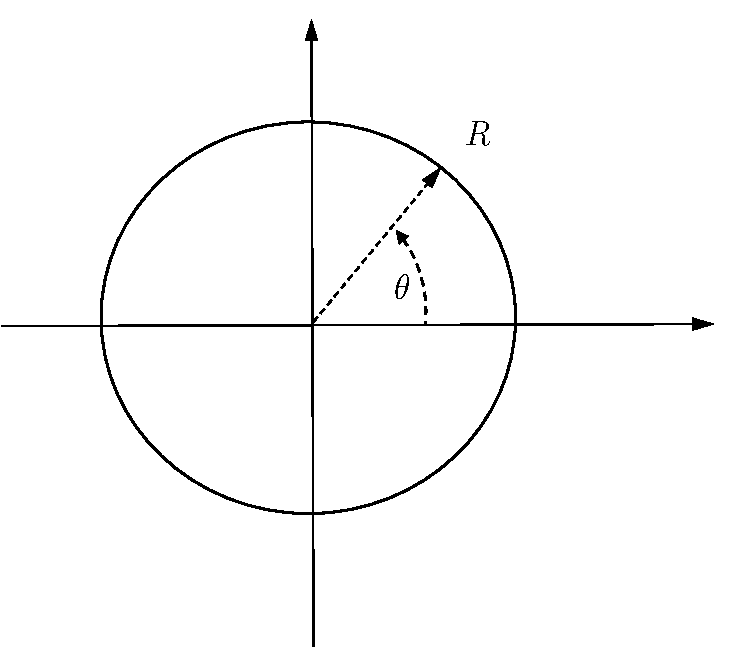
\includegraphics[width=\linewidth]{./chap2_preliminaries/figures/so_2}
  \caption{Visualization of $SO(2)$ as a point on the unit circle in $\mathbb{R}^2$.}
  \label{fig:so_2}  
\end{marginfigure}
The Lie algebra associated with $SO(2)$ is the set
\[
\so(2) = \left\{ M = \begin{pmatrix} 0 & -\theta \\ \theta & 0 \end{pmatrix} ~|~ \theta\in\mathbb{R} \right\},
\]
i.e., the set of skew-symmetric matrices in $\mathbb{R}^{2\times 2}$.  Define the ``wedge'' and ``vee'' operators as
\[
\theta^\wedge = \begin{pmatrix} 0 & -\theta \\ \theta & 0 \end{pmatrix},
\qquad \qquad
\begin{pmatrix} 0 & -\theta \\ \theta & 0 \end{pmatrix}^\vee = \theta.
\]
By straightforward manipulation, we see that 
\[
\exp(\theta^\wedge) = I + \theta^\wedge + \frac{1}{2!}(\theta^\wedge)^2 + \frac{1}{3!}(\theta^\wedge)^3 + \dots 
= \begin{pmatrix} \cos\theta & -\sin\theta \\ \sin\theta & \cos\theta \end{pmatrix}.
\]
Similarly, the $\log$ of an element of $SO(2)$ is given by
\[
\log(R) = \cos^{-1}\left(\frac{\trace{R}}{2}\right)^\wedge.
\]
It is important to note that 
\begin{align*}
\exp: &~ \so(2) \to SO(2) \\	
\log: &~ SO(2) \to \so(2),
\end{align*}
therefore it is straightforward to move back and forth between the Lie group $SO(2)$ and its Lie algebra $\so(2)$.  Note that the exponential is a many-to-one map, but that the logarithm maps elements of $SO(2)$ onto only a subset of $\so(2)$ represented by $[0,\pi]$.

It is interesting to note that $\so(2)$ is a linear vector space since linear combinations of elements in $\so(2)$ are also elements of $\so(2)$, i.e.,
\[
a\begin{pmatrix} 0 & -\theta \\ \theta & 0 \end{pmatrix} + b\begin{pmatrix} 0 & -\psi \\ \psi & 0 \end{pmatrix} = \begin{pmatrix} 0 & -(a\theta+b\psi) \\ (a\theta+b\psi) & 0 \end{pmatrix}.
\]
Note also that $\so(2)$ only has dimension of one, and that its elementary basis matrix is 
\[
J_1 = \begin{pmatrix} 0 & -1 \\ 1 & 0 \end{pmatrix}.
\]
In Lie group lingo, the basis vector $J_1$ is called the generator of $SO(2)$, because any element of $SO(2)$ can be generated by the exponential of a linear combination of the generators.  In our case, for any $M$, there exists a $\theta$ such that
\[
M = \exp(\theta J_1).
\]

Taking the derivative of $M\in SO(2)$ gives
\begin{align*}
\frac{d}{dt}\begin{pmatrix} \cos\theta & -\sin\theta \\ \sin\theta & \cos\theta \end{pmatrix} &=
	\begin{pmatrix} -\dot{\theta}\sin\theta & -\dot{\theta}\cos\theta \\ \dot{\theta}\cos\theta & -\dot{\theta}\sin\theta \end{pmatrix} \\
	&= \begin{pmatrix} \cos\theta & -\sin\theta \\ \sin\theta & \cos\theta \end{pmatrix} \begin{pmatrix} 0 & -\dot{\theta} \\ \dot{\theta} & 0 \end{pmatrix},
\end{align*}
or in other words
\[
\dot{R} = R\dot{\theta}^\wedge.
\]
Defining $\omega = \dot{\theta}$, gives
\begin{equation}\label{eq:diff_eq_so_2}
\dot{R} = R\omega^\wedge,
\end{equation}
and the solution (as seen in previous sections) is
\[
R(t) = R(t_0)\exp\left(\int_{t_0}^t \omega^\wedge(\tau)d\tau\right).
\]

Considering the differential equation $\dot{R}=R\omega^\wedge$, note that the right hand side of the equation represents a vector in the vector space that is tangent to $SO(2)$ at element $R$.  This can be visualized in Figure~\ref{fig:tangent_space_SO_2}.  Note that the tangent space is just a rotation by $R$ of the tangent space at the identity element $I$.  The tangent space at $I$ is simply $\se(2)$, which is the Lie algebra.  This is a general property of the Lie algebra of a Lie group, it is the tangent space at the identity element.
\begin{marginfigure}[0in]
  \centering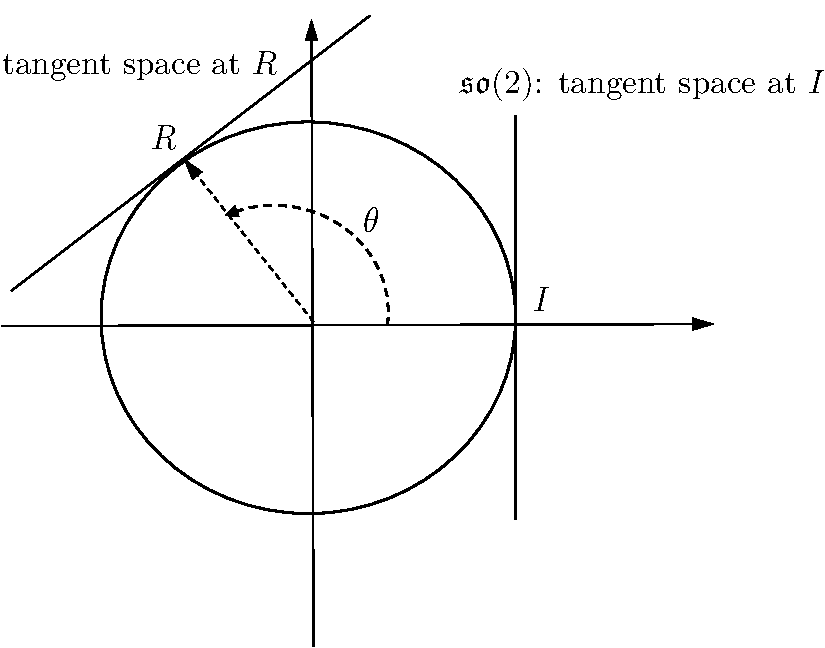
\includegraphics[width=\linewidth]{./chap2_preliminaries/figures/tangent_space_SO_2}
  \caption{Visualization of $\so(2)$ and the tangent space to $SO(2)$.}
  \label{fig:tangent_space_SO_2}  
\end{marginfigure}

Note also that if Equation~\eqref{eq:diff_eq_so_2} is multiplied on the left by a constant matrix $Q\in SO(2)$, and we let $S=QR$, then
\begin{align*}
\dot{S} &= \frac{d}{dt}(QR) 
        = Q\dot{R} 
        = QR\omega^\wedge 
        = S\omega^\wedge.
\end{align*}
Therefore $S=QR$ satisfies exactly the same differential equation as $R$.  Dynamics that not affected by a left multiplication of an element of the group are said to be {\em left-invariant} dynamics.
\marginnote{Definition of left and right invariant dynamics.}  
Similarly, if $R$ satisfies $\dot{R} = -\omega^\wedge R$, then multiplying on the right by a constant matrix $S$ does not change the dynamics, which are therefore called {\em right-invariant} dynamics.

Note that $SO(2)$ is a one-dimensional group because it can be described by a single parameter $\theta$.  We typically think of elements of $SO(2)$ as rotation matrices that transform coordinates or rotate vectors.  Therefore, associated with the vector $\wbf\in\mathbb{R}^2$, we can define the {\em group action}
\[
	f_{\wbf}(R) = R\wbf,
\]
where the output of $f_{\wbf}(R)$ is a vector that represents a transformation of $\wbf$.  However, there is a slightly different perspective here, because we think of $f$ as a function of the group element $R$, with a fixed $\wbf$, instead of as a function of $\wbf$ with a fixed $R$.  It is natural to ask whether we can take the Jacobian of the group action $f_{\wbf}$ with respect to the group element $R$.  

\marginnote{
Recall that the derivative of a function is defined as
\[
\frac{\partial f}{\partial z}=\lim_{\varepsilon\to0}\frac{f\left(z+\varepsilon\right)-f\left(z\right)}{\varepsilon}.
\]
In conversational English, this means, ``How does the output of the
function $f$ change if I bump the input a tiny amount?'' 
}
Toward that end, recall that the Jacobian of a function $g: \mathbb{R}^n\to\mathbb{R}^m$ is given by
\[
\frac{\partial g}{\partial \xbf} = \lim_{\varepsilon\to 0} \begin{pmatrix} \frac{g(\xbf+\varepsilon\ebf_1)-g(\xbf)}{\varepsilon} & \dots & \frac{g(\xbf+\varepsilon\ebf_n)-g(\xbf)}{\varepsilon}\end{pmatrix},
\]
where the $i^{th}$ row describes how  $g$ changes with incremental changes in $\xbf$ along the basis vector $\ebf_i$.  
\marginnote{
For vector functions $g:\mathbb{R}^n\to\mathbb{R}^m$, the $i^{th}$ column of the Jacobian matrix indicates how $g$ changes with as incremental change in the $i^{th}$ element of $\xbf$.
}
We can define the $\frac{\partial f}{\partial R}$ similarly, where the $i^{th}$ row of the Jacobian would describe how the group action $f_\wbf(R)$ changes incrementally as $R$ changes incrementally along the basis vector, or generator $J_i$.  In our case, there is only one generator: 
\begin{align*}
\frac{\partial f}{\partial R} &= \frac{\partial (R\wbf)}{\partial R} 
  = \lim_{\varepsilon\to 0} \frac{R\exp(\varepsilon J_1)\wbf - R\wbf}{\varepsilon} \\
  &= \lim_{\varepsilon\to 0} \frac{R\left(I + \varepsilon J_1 + \frac{\varepsilon^2}{2!}J_1^2 + \dots \right)\wbf - R\wbf}{\varepsilon} \\
  &= \lim_{\varepsilon\to 0} \frac{\varepsilon RJ_1\wbf}{\varepsilon} 
  = R J_1 \wbf.
\end{align*}
Note that $\frac{\partial f}{\partial R}$ is a $2\times 1$ vector that because $f_\wbf(R)$ maps to $\mathbb{R}^2$ (number of rows), and there is only one generator function (number of columns).
Therefore, knowing the structure (dimension and generators) of the Lie algebra is critical to the process of taking Jacobians of group actions.

\rwbcomment{add discussion on adjoints.}


%+++++++++++++++++++++++++++++++++++++++++++++++++++++++
\subsection{The Lie group $SO(3)$}

From the previous section, it should be clear that $SO(3)$ is a Lie group with matrix multiplication as the group operator.  The associated Lie algebra is $\so(3)$, the set of $3\times 3$ skew-symmetric matrices.

The exponential and logarithm functions are defined in Lemmas~\ref{lem:rodrigues_exponential} and~\ref{lem:matrix_log}.  The ``wedge'' and ``vee'' operations are defined as $\omegabf^\wedge = \ss{\omegabf}$ and Equation~\eqref{eq:vee_so_3}. Since $\Omega\in\so(3)$ implies that
\[
\Omega = \begin{pmatrix} 0 & -c & b \\ c & 0 & -b \\ -b & a & 0 \end{pmatrix},
\]
the basis vectors for $\so(3)$, or in other words, the generators for $SO(3)$ are
\begin{align*}
J_{1} & =\ebf_{1}^\wedge = \begin{pmatrix}0 & 0 & 0\\
0 & 0 & -1\\
0 & 1 & 0
\end{pmatrix}, & J_{2} &= \ebf_2^\wedge = \begin{pmatrix}0 & 0 & 1\\
0 & 0 & 0\\
-1 & 0 & 0
\end{pmatrix}, & J_{3} &= \ebf_3^\wedge = \begin{pmatrix}0 & -1 & 0\\
1 & 0 & 0\\
0 & 0 & 0
\end{pmatrix}.
\end{align*}
Therefore $\Omega\in\so(3)$ implies that
\[
\Omega = aJ_1 + bJ_2 + cJ_3,
\]
and any element $R\in SO(3)$ can be expressed as
\[
R = \exp\left( aJ_1 + bJ_2 + cJ_3 \right)
\]

If the group action is defined as $f_\wbf(R) = R\wbf$, then the Jacobian of $f$ with respect to $R$ can be computed as
\begin{align*}
\frac{\partial f}{\partial R} &= \lim_{\varepsilon \to 0} \begin{pmatrix} 
 	\frac{R\exp(\varepsilon J_1)\wbf - R\wbf}{\varepsilon} & 
 	\frac{R\exp(\varepsilon J_2)\wbf - R\wbf}{\varepsilon} &
 	\frac{R\exp(\varepsilon J_3)\wbf - R\wbf}{\varepsilon}
 \end{pmatrix} \\
 &= \lim_{\varepsilon \to 0} \begin{pmatrix} 
 	\frac{\varepsilon RJ_1\wbf}{\varepsilon} & 
 	\frac{\varepsilon RJ_2\wbf}{\varepsilon} &
 	\frac{\varepsilon RJ_3\wbf}{\varepsilon}
 \end{pmatrix}
  = R\begin{pmatrix} 
 	\ebf_1^\wedge\wbf & 
 	\ebf_2^\wedge\wbf & 
 	\ebf_3^\wedge\wbf 
 \end{pmatrix} \\
 &= R\begin{pmatrix} 
 	\wbf^\wedge\ebf_1 & 
 	\wbf^\wedge\ebf_2 & 
 	\wbf^\wedge\ebf_3 
 \end{pmatrix} 
  = R\wbf^\wedge \begin{pmatrix} 
 	\ebf_1 & 
 	\ebf_2 & 
 	\ebf_3 
 \end{pmatrix}\\
   &= -R\wbf^\wedge.
\end{align*}

\rwbcomment{Need to explain other Jacobians in table at end of section.}
\rwbcomment{Need to explain adjoint.}
\rwbcomment{Need to explain right Jacobian vs. left Jacobian.}


%
%
%As mentioned before, all members of a Lie group can be created by
%computing the exponential of a linear combination of the generators.
%Furthermore, because the generators are orthogonal, $\so\left(3\right)$
%is isomorphic to $\mathbb{R}^{3}$. Therefore, to keep things concise, we
%can actually form a vector whose coefficients are then multiplied
%by the generators. In the case of $SO(3)$, this is the
%same as computing the skew-symmetric matrix of a vector. But in general,
%the $\left(\cdot\right)^{\wedge}$ and $\left(\cdot\right)^{\vee}$
%notation is used to indicate this mapping. For example, for $\so\left(3\right):$
%
%\begin{align*}
%\left(\vbf^{\wedge}\right) & =\sum_{i}J_{i}\ebf_{i}^{\top}\vbf\\
% & =J_{1}\vbf_{x}+J_{2}\vbf_{y}+J_{3}\vbf_{z}\\
% & =\begin{pmatrix}0 & -\vbf_{z} & \vbf_{y}\\
%\vbf_{z} & 0 & -\vbf_{x}\\
%-\vbf_{y} & -\vbf_{x} & 0
%\end{pmatrix},
%\end{align*}
%
%\[
%\left(\vbf^{\wedge}\right)^{\vee}=\vbf.
%\]
%This notation is used in some literature \cite{Barfoot2019,Sola2019},
%but not in others \cite{Drummond2014,Ethan2019}. Since the two representations
%(the matrix algebra and the vector) are isomorphic, the mapping to
%the matrix Lie Algebra is often skipped notationally, and $\exp\left(\vbf\right)$
%is written while $\exp\left(\vbf^{\wedge}\right)$ would technically
%be more correct. As computing the matrix exponential of $\vbf\in\mathbb{R}^{3}$
%is actually not possible given the definition above, the mapping of
%the vector to the matrix Lie Algebra is implied in literature where
%the mapping is ignored.

%+++++++++++++++++++++++++++++++++++++++++++++++++++++++
\subsection{The Lie group $SE(3)$}

\rwbcomment{rewrite this section}

As mentioned before, $SE(3)$ is the set of rigid body
transforms. Lie Theory as developed by physicists has very little
to say about $SE(3)$, as it is actually a subset of the
set of $4\times4$ matrices, known classically as the Lorentz group.
The Lorentz group (or the complexified version, octonians) are used
to encode not only rigid body transforms, but also the dilation of
space and time due to relativistic effects. In robotics, we can usually
restrict ourselves to time and space-preserving transformations, so
we can use a simplified version of the Lorentz space generators.\footnote{The bottom row of the $4\times4$ matrix is used in the Lorentz group,
whereas is it not used in $SE(3).$ The Lorentz group
generators continue the skew-symmetric pattern we are used to in this
bottom row and right column. For more information about using Lie
groups to model spacetime, \cite{schwichtenberg_2015} is a phenomenal
introductory text to Lie groups in the context of theoretical physics.
It includes a very good explanation of the Lorentz group and its double-cover.} 

The generators of $SE(3)$ are just the basis of infinitesimal
transformations along each degree of freedom.

\begin{align*}
J_{1} & =\begin{pmatrix}0 & 0 & 0 & 0\\
0 & 0 & -1 & 0\\
0 & 1 & 0 & 0\\
0 & 0 & 0 & 0
\end{pmatrix} & J_{2} & =\begin{pmatrix}0 & 0 & 1 & 0\\
0 & 0 & 0 & 0\\
-1 & 0 & 0 & 0\\
0 & 0 & 0 & 0
\end{pmatrix} & J_{3} & =\begin{pmatrix}0 & -1 & 0 & 0\\
1 & 0 & 0 & 0\\
0 & 0 & 0 & 0\\
0 & 0 & 0 & 0
\end{pmatrix}\\
J_{4} & =\begin{pmatrix}0 & 0 & 0 & 1\\
0 & 0 & 0 & 0\\
0 & 0 & 0 & 0\\
0 & 0 & 0 & 0
\end{pmatrix} & J_{5} & =\begin{pmatrix}0 & 0 & 0 & 0\\
0 & 0 & 0 & 1\\
0 & 0 & 0 & 0\\
0 & 0 & 0 & 0
\end{pmatrix} & J_{6} & =\begin{pmatrix}0 & 0 & 0 & 0\\
0 & 0 & 0 & 0\\
0 & 0 & 0 & 1\\
0 & 0 & 0 & 0
\end{pmatrix}.
\end{align*}
The use of these generators defines the $\left(\cdot\right)^{\wedge}$
operator for $SE(3)$ as

\[
\begin{pmatrix}\omegabf\\
\vbf
\end{pmatrix}^{\wedge}=\begin{pmatrix}\ss{\omegabf} & \vbf\\
0 & 0
\end{pmatrix},
\]
and $\left(\cdot\right)^{\vee}$ as the inverse operation.



%+++++++++++++++++++++++++++++++++++++++++++++++++++++++
\subsection{The Lie group $S^3$}

\rwbcomment{rewrite this section}

%++++++++++++++++++++++++++++++++++++++
\subsection{Closed-Form Exponential for $\protect S^{3}$}

Let's start with the definition of the quaternion exponential

\begin{align}
\exp\left(\omegabf^{\wedge}\right) & =\sum_{k=0}^{\infty}\frac{\left(\omegabf^{\wedge}\right)^{k}}{k!}, & \omegabf^{\wedge} & =\begin{pmatrix}0\\
\omegabf
\end{pmatrix}\label{eq:quat_exp_series}
\end{align}
where the term $\left(\qbf\right)^{k}$ refers to multiplying $\qbf$
with itself $\left(\qbf\cdot\qbf\cdot\cdots\right)$ $k$ times. We also
note that

\begin{align*}
\left(\omegabf^{\wedge}\right)^{2} & =\left(\omegabf_{x}i+\omegabf_{y}j+\omegabf_{z}k\right)\cdot\left(\omegabf_{x}i+\omegabf_{y}j+\omegabf_{z}k\right)\\
 & =-\omegabf_{x}^{2}-\omegabf_{d}^{2}-\omegabf_{z}^{2}\\
 & =-\norm{\omegabf}^{2}
\end{align*}
Therefore, if $\theta=\norm{\omegabf}$, then

\begin{align*}
\left(\omegabf^{\wedge}\right)^{2} & =-\theta^{2}, & \left(\omegabf^{\wedge}\right)^{3} & =-\theta^{2}\omegabf^{\wedge} & \left(\omegabf^{\wedge}\right)^{4} & =\theta^{4}\cdots.
\end{align*}
Now, we can rewrite the series in Eq. \ref{eq:quat_exp_series} as

\begin{align}
\exp\left(\omegabf^{\wedge}\right) & =\sum_{k=0}^{\infty}\frac{\left(\omegabf^{\wedge}\right)^{k}}{k!}\nonumber \\
 & =1+\omegabf^{\wedge}-\frac{\theta^{2}}{2!}-\frac{\theta^{2}}{3!}\omegabf^{\wedge}+\frac{\theta^{4}}{4!}+\frac{\theta^{4}}{5!}\omegabf^{\wedge}-\cdots\nonumber \\
 & =1+\frac{\theta}{\theta}\omegabf^{\wedge}-\frac{\theta^{2}}{2!}-\frac{\theta^{3}}{3!\theta}\omegabf^{\wedge}+\frac{\theta^{4}}{4!}+\frac{\theta^{5}}{5!\theta}\omegabf^{\wedge}-\cdots\nonumber \\
 & =\left(1-\frac{\theta^{2}}{2!}+\frac{\theta^{4}}{4!}\cdots\right)+\frac{1}{\theta}\left(\theta-\frac{\theta^{3}}{3!}+\frac{\theta^{5}}{5!}\cdots\right)\omegabf^{\wedge}\nonumber \\
 & =\cos\left(\theta\right)+\frac{\sin\left(\theta\right)}{\theta}\omegabf^{\wedge}.\label{eq:quat_exp}
\end{align}
As with the rotation matrix exponential, we will want to use the Taylor
series approximation if $\theta\approx0$ to avoid numerical errors.
(See Table \ref{tab:taylor_series}).

Computing the closed-form logarithm is done by inverting Eq. \ref{eq:quat_exp}
and is given by

\[
\log\left(\qbf\right)=\textnormal{atan2}\left(\norm{\vec{\qbf}},q_{0}\right)\frac{\qbf}{\norm{\vec{\qbf}}}.
\]
Because of the fact that quaternion dynamics have a $\frac{1}{2}$
in front of them (See Eq. \ref{eq:quaternion_dynamics}), it is common
practice in both physics and robotics applications to embed the $\frac{1}{2}$
into the $\exp$ function itself such that\footnote{You might recognize this as the axis-angle conversion to unit quaternions
(Eq. \ref{eq:quat_axis_angle})}

\[
\boxed{\exp\left(\omegabf\right)=\cos\left(\frac{\norm{\omegabf}}{2}\right)+\sin\left(\frac{\norm{\omegabf}}{2}\right)\frac{\omegabf}{\norm{\omegabf}}}
\]

\[
\boxed{\log\left(\qbf\right)=2\tan^{-1}\left(\frac{\norm{\vec{\qbf}}}{q_{0}}\right)\cdot\frac{\vec{\qbf}}{\norm{\vec{\qbf}}}.}
\]
This is actually the same as if we redefined the generators of the
unit quaternion to all be $\frac{1}{2}J_{i}$. This is fine, and totally
proper, however we just need to be explicit about this choice.

%-----------------------------------------------------------------
\section{The Adjoint as the Jacobian of Group Action}

\rwbcomment{move this stuff up into the previous sections}

\label{sec:ad_as_jacobian}



The concept of differentiation works quite naturally with Lie groups
as well. For example, consider the case of some function $h\in SE(3)\to\mathbb{R}^{n}.$
What we want is a matrix that tells us how the output of $h$ behaves
as we tweak the argument of $h$ along the \emph{generators }of $\se\left(3\right).$
To compute this, we use the fact that every member of the group can
be described by the exponential of some linear combination of generators,
as in

\begin{align*}
T & =\exp\left(\xbf^{\wedge}\right), & \xbf^{\wedge} & =\log\left(T\right).
\end{align*}
When we write it this way, we can see how we might perturb $\xbf$ (and
therefore, $T$) in the $J_{i}$ direction:

\begin{align*}
T_{i}^{+} & =\exp\left(\xbf^{\wedge}+J_{i}\varepsilon\right)\\
 & =T\cdot\exp\left(J_{i}\varepsilon\right).
\end{align*}
Next, we need to think about how we might compute the difference between
$T_{i}^{+}$ and the original $T$. Again, looking to the Lie Algebra,
we should expect the difference $\deltabf_{i}\in\se\left(3\right)$ to
be

\begin{align}
\exp\left(\deltabf_{i}\right) & =T\cdot\exp\left(J_{i}\varepsilon\right)\cdot\exp\left(-\xbf^{\wedge}\right)\nonumber \\
\deltabf_{i} & =\log\left(T\cdot\exp\left(J_{i}\varepsilon\right)\cdot T^{-1}\right)^{\vee}.\label{eq:adjoint_start}
\end{align}
If we make a matrix out of the six $\deltabf_{i}$ for $\se\left(3\right)$,
take the limit as $\varepsilon\to0$ and attach coordinate frames
to our transform $T_{a}^{b}$, then we get a $6\times6$ matrix that
tells us how things change along the generators in the $b$ frame
if we perturb along the generators the $a$ frame. This has a special
name--the Adjoint--and it just so happens to be the Jacobian of
the group action by a member of the group.

We can come at the Adjoint in another way: because the Adjoint is
the Jacobian of the group action of a Lie group, we can use it to
map vectors from the ``output'' of a group action to the ``input'',
and vice-versa. In mathematical terms\footnote{for the rest of this section, I'm dropping the $\left(\cdot\right)^{\wedge}$
so we can focus on the coordinate frame notation. The mapping from
the vector to algebra should be implied by context.}:

\[
T\cdot\exp\left(\deltabf\right)=\exp\left(\Ad_{T}\cdot\deltabf\right)\cdot T.
\]
See how we have ``moved'' $\deltabf$ from the ``input'' of $T$ (the
right side) to the ``output'' (the left side)? If we attach coordinate
frames to $T$ this becomes even more clear: 

\begin{align}
T_{a}^{b}\cdot\exp\left(\deltabf^{a}\right) & =\exp\left(\Ad\left(T_{a}^{b}\right)\cdot\deltabf^{a}\right)\cdot T_{a}^{b}.\nonumber \\
 & =\exp\left(\deltabf^{b}\right)\cdot T_{a}^{b}.\label{eq:adjoint_show}
\end{align}
The Adjoint transforms $\deltabf$ from $a$ to $b.$

Remember all that talk about left-invariance and right-invariance?
This property of the Adjoint of the Lie Group lets us swap back and
forth however we need to. This is really helpful when computing Jacobians
of complex expressions involving Lie Groups.

\section{Closed-Form Expressions for the Adjoint}

In this section, I'm going to derive the Adjoint for each of our four
Lie Groups, but before we do that,\emph{ }let's first talk about a
concrete example of where the Adjoint is useful. 

Let's consider some kind of nonlinear controller that is computing
error on the Lie Algebra of $SE(3)$, where we have some
desired state $\check{T}$ and our current state $T.$ We're going
to form some control law around the error between these two states.
Naturally, we want to use linear algebra as the backbone of our implementation,
so we'd like to use $\se\left(3\right)^{\vee}$ to represent our error.
We could compute the error in one of 4 ways:

\begin{align*}
\deltabf_{a}^{\check{a}} & =\log\left(\check{\left(T_{a}^{b}\right)}^{-1}\cdot T_{a}^{b}\right)\\
\deltabf_{b}^{\check{b}} & =\log\left(\check{T_{a}^{b}}\cdot\left(T_{a}^{b}\right)^{-1}\right)\\
\deltabf_{\check{a}}^{a} & =\log\left(\left(T_{a}^{b}\right)^{-1}\cdot\check{T_{a}^{b}}\right)\\
\deltabf_{\check{b}}^{b} & =\log\left(\left(T_{a}^{b}\right)\cdot\left(\check{T}_{a}^{b}\right)^{-1}\right).
\end{align*}
The choice of error depends largely on which frames are moving, and
which are not. Let's assume that in this case the $a$ frame is shared
between the transform (i.e. perhaps $a$ refers to the inertial frame),
and that the $b$ and $\check{b}$ frames are the current and desired
body frame of a robot. The goal of the controller in this case is
to make $b=\check{b}.$ In this case, it makes the most sense to define
our error as one of the following two options (or else the coordinate
frames will not match up):

\begin{align*}
\deltabf_{b}^{\check{b}} & =\log\left(\check{T_{a}^{b}}\cdot\left(T_{a}^{b}\right)^{-1}\right),\\
\deltabf_{\check{b}}^{b} & =\log\left(T_{a}^{b}\cdot\left(\check{T}_{a}^{b}\right)^{-1}\right).
\end{align*}
Driving either of these errors to zero will achieve our control objectives.
However, watch what happens when we want to compute the Jacobian of
our error with respect to our current state. We can find these Jacobians
using the chain rule: 

\begin{align*}
\frac{\partial}{\partial T_{a}^{b}}\deltabf_{b}^{\check{b}} & =\left.\frac{\partial\log\left(\xbf\right)}{\partial\xbf}\right|_{\xbf=\left(T_{a}^{b}\cdot\left(T_{a}^{\check{b}}\right)\right)}\cdot\frac{\partial}{\partial T_{a}^{b}}\left(\check{T_{a}^{b}}\cdot\left(T_{a}^{b}\right)^{-1}\right) & =A\cdot B^{\check{b}}\\
\frac{\partial}{\partial T_{a}^{b}}\deltabf_{\check{b}}^{b} & =\left.\frac{\partial\log\left(\xbf\right)}{\partial\xbf}\right|_{\xbf=\left(T_{a}^{b}\cdot\left(T_{a}^{\check{b}}\right)\right)}\cdot\frac{\partial}{\partial T_{a}^{b}}\left(T_{a}^{b}\cdot\left(\check{T_{a}^{b}}\right)^{-1}\right) & =A\cdot B^{b}
\end{align*}

The expression for $A$ is in Table \ref{tab:lie_identities_group_vector-se3},
and it's the same for both parameterizations. However, we are left
with the two $B$ expressions. In the first case, we have to go through
our desired state to get to the current state. This isn't too bad,
we just look at Table \ref{tab:lie_identities_group_operations} to
get (using the left Jacobian):

\begin{align*}
B^{\check{b}} & =\frac{\partial}{\partial T_{a}^{b}}\left(\check{T_{a}^{b}}\cdot\left(T_{a}^{b}\right)^{-1}\right)\\
 & =-\Ad\left(\check{T_{a}^{b}}\cdot\left(T_{a}^{b}\right)^{-1}\right)
\end{align*}
for the first cast, and

\begin{align*}
B^{b} & =\frac{\partial}{\partial T_{a}^{b}}\left(T_{a}^{b}\cdot\left(\check{T_{a}^{b}}\right)^{-1}\right)\\
 & =I\in\mathbb{R}^{6\times6}.
\end{align*}
for the second. Having a closed form expression for the Adjoint makes
computing these kinds of expressions very straight-forward. 

Most modern forms of control and estimation rely heavily on quickly-computed
Jacobians. With a table of Jacobians for exp, log, Ad and a few other
Lie group expressions, plus the Matrix Cookbook \cite{Petersen2012},
it's pretty easy to chain-rule out even the hairiest Jacobians pretty
quickly to get analytical expressions. Appendix \ref{sec:Tables}
contains most of these Jacobians for easy reference.

\subsection{Adjoint for $SO(3)$}

For all four Lie groups, we can derive the Adjoint by finding the
closed-form expression of Eq. \ref{eq:adjoint_start}. $SO(3)$
is quite easy:

\begin{align*}
\Ad\left(R\right) & =\lim_{\varepsilon\to0}\frac{1}{\varepsilon}\begin{bmatrix}R\cdot\exp\left(J_{1}\varepsilon\right)\cdot R^{-1} & \cdots\end{bmatrix}\\
 & =\lim_{\varepsilon\to0}\frac{1}{\varepsilon}\begin{bmatrix}R\cdot\left(I+\ss{\ebf_{1}\epsilon}+\cdots\right)\cdot R^{-1} & \cdots\end{bmatrix}\\
 & =\lim_{\varepsilon\to0}\frac{1}{\varepsilon}\begin{bmatrix}R\cdot R^{-1}+R\cdot\ss{\ebf_{1}\epsilon}\cdot R^{-1} & \cdots\end{bmatrix}\\
 & =\begin{bmatrix}R\cdot\ss{\ebf_{1}}\cdot R^{-1} & \cdots\end{bmatrix} & R\cdot R^{-1}=I\\
 & =\begin{bmatrix}\ss{R\ebf_{1}} & \ss{R\ebf_{2}} & \ss{R\ebf_{3}}\end{bmatrix} & \textnormal{(Eq. \ref{eq:skew_trick_2})}\\
 & =R
\end{align*}
We see here that $SO(3)$ is \emph{self-adjoint}, and
it makes sense why. Consider an $SO(3)$ version of Eq.
\ref{eq:adjoint_show}. Rotating the vector is the natural way to
transform $\deltabf$ from the $a$ frame to the $b$ frame.

\[
\boxed{\Ad\left(R\right)=R}
\]


\subsection{Adjoint for Unit Quaternions}

Remember, the Adjoint action is given by 

\[
\Ad=\lim_{\varepsilon\to0}\frac{1}{\varepsilon}\begin{bmatrix}\log\left(\qbf\cdot\exp\left(J_{1}\varepsilon\right)\cdot\qbf^{-1}\right) & \cdots\end{bmatrix}.
\]
In the case of unit quaternions, we can see that they too, are self-adjoint.
To compute the adjoint of a quaternion, all we need to do is pre-
and post-multiply a pure quaternion of the lie algebra member by the
quaternion. 

\[
\Ad\left(\qbf\right)=\qbf\cdot\deltabf\cdot\qbf^{-1}.
\]
However, sometimes we might want the matrix form of the adjoint. This
can be computed as follows:

\begin{align*}
 & =\lim_{\varepsilon\to 0}\frac{1}{\varepsilon}\begin{bmatrix}\log\left(\qbf\cdot\begin{pmatrix}0\\
\ebf_{1}\sin\left(\frac{\varepsilon}{2}\right)
\end{pmatrix}\cdot\qbf^{-1}\right) & \cdots\end{bmatrix}\\
 & =\lim_{\varepsilon\to 0}\frac{1}{\varepsilon}\begin{bmatrix}\log\begin{pmatrix}0\\
\frac{R^{\top}\ebf_{1}\varepsilon}{2}
\end{pmatrix} & \cdots\end{bmatrix}\\
 & =\lim_{\varepsilon\to 0}\frac{1}{\varepsilon}\begin{bmatrix}R^{\top}\ebf_{1}\varepsilon & R^{\top}\ebf_{2}\varepsilon & R^{\top}\ebf_{3}\varepsilon\end{bmatrix}\\
 & =R^{\top}.
\end{align*}
You could probably come up with this only just from intuition as well.
If you remember that quaternions and rotation matrices share a Lie
Algebra, and that the order of concatenation is backwards, then $R^{\top}$
is the logical choice.

\[
\boxed{\Ad\left(\qbf\right)=R^{\top}\left(\qbf\right)}
\]


\subsection{Adjoint for $SE(3)$}

Computing this adjoint is more complicated than pure rotation. Unfortunately,
$SE(3)$ isn't self-adjoint,\footnote{This should be pretty obvious, seeing as $\se\left(3\right)$ is 6-dimensional
while $SE(3)$ is a group of $4\times4$ matrices.} so the limit gets a little more hairy. We have two main blocks: the
first three generators are the rotation generators, while the last
three are the translation generators. Let's consider these separately.
First, the rotation blocks

\begin{align*}
\Ad_{1-3} & =\lim_{\varepsilon\to0}\frac{1}{\varepsilon}\begin{bmatrix}\log\left(T\cdot\exp\left(J_{1}\varepsilon\right)\cdot T^{-1}\right) & \cdots\end{bmatrix}\\
 & =\lim_{\varepsilon\to0}\frac{1}{\varepsilon}\begin{bmatrix}\log\left(T\cdot\begin{bmatrix}\ss{\ebf_{1}\varepsilon} & 0\\
0 & 0
\end{bmatrix}\cdot T^{-1}\right) & \cdots\end{bmatrix}\\
 & =\lim_{\varepsilon\to0}\frac{1}{\varepsilon}\begin{bmatrix}\log\left(\begin{bmatrix}R & \tbf\\
0 & 1
\end{bmatrix}\cdot\begin{bmatrix}\ss{\ebf_{1}\varepsilon} & 0\\
0 & 0
\end{bmatrix}\cdot\begin{bmatrix}R^{\top} & -R^{\top}\tbf\\
0 & 1
\end{bmatrix}\right) & \cdots\end{bmatrix}\\
 & =\lim_{\varepsilon\to0}\frac{1}{\varepsilon}\begin{bmatrix}\log\left(\begin{bmatrix}R\ss{\ebf_{1}\varepsilon} & 0\\
0 & 0
\end{bmatrix}\cdot\begin{bmatrix}R^{\top} & -R^{\top}\tbf\\
0 & 1
\end{bmatrix}\right) & \cdots\end{bmatrix}\\
 & =\lim_{\varepsilon\to0}\frac{1}{\varepsilon}\begin{bmatrix}\log\left(\begin{bmatrix}R\ss{\ebf_{1}\varepsilon}R^{\top} & -R\ss{\ebf_{1}\varepsilon}R^{\top}\tbf\\
0 & 0
\end{bmatrix}\right) & \cdots\end{bmatrix}\\
 & =\lim_{\varepsilon\to0}\frac{1}{\varepsilon}\begin{bmatrix}\log\left(\begin{bmatrix}\ss{R\ebf_{1}\varepsilon} & -\ss{R\ebf_{1}\varepsilon}\tbf\\
0 & 0
\end{bmatrix}\right) & \cdots\end{bmatrix} & \textnormal{(Eq. \ref{eq:skew_trick_2})}\\
 & =\lim_{\varepsilon\to0}\frac{1}{\varepsilon}\begin{bmatrix}\log\left(\begin{bmatrix}\ss{R\ebf_{1}\varepsilon} & \ss{\tbf}R\ebf_{1}\varepsilon\\
0 & 0
\end{bmatrix}\right) & \cdots\end{bmatrix} & \textnormal{(Eq. \ref{eq:skew_trick_1})}\\
 & =\lim_{\varepsilon\to0}\frac{1}{\varepsilon}\begin{bmatrix}R\varepsilon\\
\ss{\tbf}R\varepsilon
\end{bmatrix}\\
 & =\begin{bmatrix}R\\
\ss{\tbf}R
\end{bmatrix}.
\end{align*}
Now for the translation blocks

\begin{align*}
\Ad_{4-6} & =\lim_{\varepsilon\to0}\frac{1}{\varepsilon}\begin{bmatrix}\log\left(T\cdot\exp\left(J_{4}\varepsilon\right)\cdot T^{-1}\right) & \cdots\end{bmatrix}\\
 & =\lim_{\varepsilon\to0}\frac{1}{\varepsilon}\begin{bmatrix}\log\left(\begin{bmatrix}R & \tbf\\
0 & 1
\end{bmatrix}\cdot\begin{bmatrix}0 & \ebf_{1}\varepsilon\\
0 & 0
\end{bmatrix}\cdot\begin{bmatrix}R^{\top} & -R^{\top}\tbf\\
0 & 1
\end{bmatrix}\right) & \cdots\end{bmatrix}\\
 & =\lim_{\varepsilon\to0}\frac{1}{\varepsilon}\begin{bmatrix}\log\left(\begin{bmatrix}0 & R\ebf_{1}\varepsilon\\
0 & 0
\end{bmatrix}\cdot\begin{bmatrix}R^{\top} & -R^{\top}\tbf\\
0 & 1
\end{bmatrix}\right) & \cdots\end{bmatrix}\\
 & =\lim_{\varepsilon\to0}\frac{1}{\varepsilon}\begin{bmatrix}\log\left(\begin{bmatrix}0 & R\ebf_{1}\varepsilon\\
0 & 0
\end{bmatrix}\right) & \cdots\end{bmatrix}\\
 & =\lim_{\varepsilon\to0}\frac{1}{\varepsilon}\begin{bmatrix}0 & 0 & 0\\
R\ebf_{1}\varepsilon & R\ebf_{2}\varepsilon & R\ebf_{3}\varepsilon
\end{bmatrix}\\
 & =\begin{bmatrix}0\\
R
\end{bmatrix}.
\end{align*}
We now concatenate these blocks to get the final Adjoint matrix:

\[
\boxed{\Ad\left(T\right)=\begin{pmatrix}R & 0\\
\ss{\tbf}R & R
\end{pmatrix}.}
\]
Note that some literature\cite{Drummond2014,Ethan2019} derives this
block-transposed. All that means is that they define generators 1-3
as the translation generators and 4-6 as the rotation generators.

Before moving on, let's take a second to develop a little bit of intuition
regarding the adjoint when it comes to rigid transforms. Consider
a rod rotating about a fixed origin, as shown in Figure \ref{fig:rotating_adjoint}.
Let us say we have the linear and angular velocity of coordinate frame
$a$, but we want the velocity of coordinate frame $b$. Because the
coordinate frames are fixed by some rigid transform, any angular rate
value of $a$ is the same for $b$, only rotated. However, to compute
the linear velocity of coordinate frame $b$, we must account for
the ``lever arm'' and the angular rate. This is what is going on
in the bottom-left corner of the Adjoint in $SE(3).$ 

\begin{marginfigure}
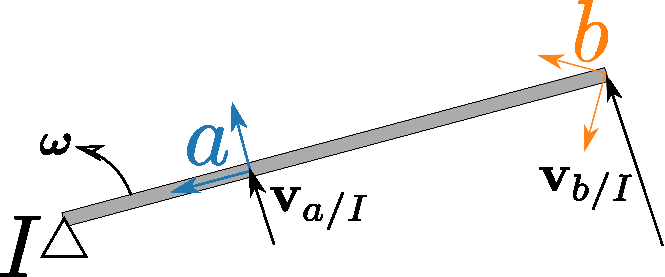
\includegraphics[width=\linewidth]{chap2_preliminaries/figures/rotating_bar}
\caption{Illustration of a rotating rigid body with two coordinate frames.
The Adjoint of $SE(3)$ will convert $\omegabf$
and $\vbf$ from frame $a$ to frame $b$, and account for the
change in translation. }
\label{fig:rotating_adjoint}
\end{marginfigure}

%++++++++++++++++++++++++++++++++++++++++++++++++++++++++
%\subsection{Adjoint of Dual Quaternions}
%
%As with unit quaternions, dual unit quaternions are also self-adjoint:
%
%\[
%\Ad\left(\Gamma\right)=\Gamma\cdot\exp\left(\dbf\right)\cdot\Gamma^{-1}.
%\]
%We have no problem dealing with six-vectors here (the problem with
%$SE(3),$which led us to compute that hairy limit). However,
%just like unit quaternions, we can compute the matrix form of the
%Adjoint using the limit expression. Again, let's split up the generators
%into two groups to help keep things a little more concise
%
%{\small{}
%\begin{align*}
%\Ad_{1-3} & =\lim_{\varepsilon\to0}\frac{1}{\varepsilon}\begin{bmatrix}\log\left(\Gamma\cdot\exp\left(J_{1}\varepsilon\right)\cdot\Gamma^{-1}\right) & \cdots\end{bmatrix}\\
% & =\lim_{\varepsilon\to0}\frac{1}{\varepsilon}\begin{bmatrix}\log\left(\begin{bmatrix}\qbf_{r}\\
%\epsilon\qbf_{d}
%\end{bmatrix}\cdot\begin{bmatrix}\begin{pmatrix}0\\
%\ebf_{1}\sin\left(\frac{\varepsilon}{2}\right)
%\end{pmatrix}\\
%0\epsilon
%\end{bmatrix}\cdot\begin{bmatrix}\qbf_{r}\\
%\epsilon\qbf_{d}
%\end{bmatrix}^{-1}\right) & \cdots\end{bmatrix}\\
% & =\lim_{\varepsilon\to0}\frac{1}{\varepsilon}\begin{bmatrix}\log\left(\begin{bmatrix}\qbf_{r}\\
%\epsilon\qbf_{d}
%\end{bmatrix}\cdot\begin{bmatrix}\ebf_{1}\varepsilon\\
%0\epsilon
%\end{bmatrix}\cdot\begin{bmatrix}\qbf_{r}\\
%\epsilon\qbf_{d}
%\end{bmatrix}^{-1}\right) & \cdots\end{bmatrix} & \sin\varepsilon\to\varepsilon\\
% & =\lim_{\varepsilon\to0}\frac{1}{\varepsilon}\begin{bmatrix}\log\left(\begin{bmatrix}\qbf_{r}\cdot\ebf_{1}^{\wedge}\varepsilon\\
%\epsilon\left(\ebf_{1}^{\wedge}\varepsilon\cdot\qbf_{d}\right)
%\end{bmatrix}\cdot\begin{bmatrix}\qbf_{r}\\
%\epsilon\qbf_{d}
%\end{bmatrix}^{-1}\right) & \cdots\end{bmatrix}\\
% & =\lim_{\varepsilon\to0}\frac{1}{\varepsilon}\begin{bmatrix}\log\left(\begin{bmatrix}\qbf_{r}\cdot\ebf_{1}^{\wedge}\varepsilon\cdot\qbf_{r}^{-1}\\
%\epsilon\left(\qbf_{r}\cdot\ebf_{1}^{\wedge}\varepsilon\cdot\qbf_{d}^{-1}+\qbf_{r}^{-1}\cdot\ebf_{1}^{\wedge}\varepsilon\cdot\qbf_{d}\right)
%\end{bmatrix}\right) & \cdots\end{bmatrix} & \ebf_{1}^{\wedge}=\begin{pmatrix}0\\
%\ebf_{1}
%\end{pmatrix}\\
% & =\lim_{\varepsilon\to0}\frac{1}{\varepsilon}\begin{bmatrix}\log\left(\begin{bmatrix}\qbf_{r}\cdot\ebf_{1}^{\wedge}\varepsilon\cdot\qbf_{r}^{-1}\\
%\epsilon\left(\qbf_{r}\cdot\ebf_{1}^{\wedge}\varepsilon\cdot\begin{pmatrix}\frac{1}{2}\t^{\wedge}\cdot\qbf_{r}\end{pmatrix}^{-1}+\qbf_{r}^{-1}\cdot\ebf_{1}^{\wedge}\varepsilon\cdot\frac{1}{2}\t^{\wedge}\cdot\qbf_{r}\right)
%\end{bmatrix}\right) & \cdots\end{bmatrix}\\
% & =\lim_{\varepsilon\to0}\frac{1}{\varepsilon}\begin{bmatrix}\log\left(\begin{bmatrix}\qbf_{r}\cdot\ebf_{1}^{\wedge}\varepsilon\cdot\qbf_{r}^{-1}\\
%\frac{1}{2}\epsilon\left(\qbf_{r}\cdot\ebf_{1}^{\wedge}\varepsilon\cdot\qbf_{r}^{-1}\cdot\left(-\t^{\wedge}\right)+\qbf_{r}^{-1}\cdot\ebf_{1}^{\wedge}\varepsilon\cdot\t^{\wedge}\cdot\qbf_{r}\right)
%\end{bmatrix}\right) & \cdots\end{bmatrix}\\
% & =\lim_{\varepsilon\to0}\frac{1}{\varepsilon}\begin{bmatrix}\log\left(\begin{bmatrix}\qbf_{r}\cdot\ebf_{1}^{\wedge}\varepsilon\cdot\qbf_{r}^{-1}\\
%\frac{1}{2}\epsilon\left(-\ss{R^{\top}\ebf_{1}\varepsilon}\tbf+R\ss{\ebf_{1}\varepsilon}\tbf\right)
%\end{bmatrix}\right) & \cdots\end{bmatrix} & \textnormal{(Eq. \ref{eq:quat_mult_matrix})}\\
% & =\lim_{\varepsilon\to0}\frac{1}{\varepsilon}\begin{bmatrix}\log\left(\begin{bmatrix}\qbf_{r}\cdot\ebf_{1}^{\wedge}\varepsilon\cdot\qbf_{r}^{-1}\\
%\frac{1}{2}\epsilon\left(-R^{\top}\ss{\ebf_{1}\varepsilon}R\tbf+R\ss{\ebf_{1}\varepsilon}\tbf\right)
%\end{bmatrix}\right) & \cdots\end{bmatrix} & \textnormal{(Eq. \ref{eq:skew_trick_2})}\\
% & =\lim_{\varepsilon\to0}\frac{1}{\varepsilon}\begin{bmatrix}\log\left(\begin{bmatrix}\qbf_{r}\cdot\ebf_{1}^{\wedge}\varepsilon\cdot\qbf_{r}^{-1}\\
%\frac{1}{2}\epsilon\left(R^{\top}\ss{R\t}\ebf_{1}\varepsilon-R\ss{\tbf}\ebf_{1}\varepsilon\right)
%\end{bmatrix}\right) & \cdots\end{bmatrix} & \textnormal{(Eq. \ref{eq:skew_trick_1})}\\
% & =\lim_{\varepsilon\to0}\frac{1}{\varepsilon}\begin{bmatrix}\log\left(\begin{bmatrix}\qbf_{r}\cdot\ebf_{1}^{\wedge}\varepsilon\cdot\qbf_{r}^{-1}\\
%\frac{1}{2}\epsilon\left(\ss{\tbf}R^{\top}\ebf_{1}\varepsilon-R\ss{\tbf}\ebf_{1}\varepsilon\right)
%\end{bmatrix}\right) & \cdots\end{bmatrix} & \textnormal{(Eq. \ref{eq:skew_trick_1})}\\
% & =\begin{bmatrix}R^{\top}\\
%\ss{\tbf}R^{\top}
%\end{bmatrix}.
%\end{align*}
%Whew! Luckily, the translation generators are much easier:}{\small\par}
%
%\begin{align*}
%\Ad_{4-6} & =\lim_{\varepsilon\to0}\frac{1}{\varepsilon}\begin{bmatrix}\log\left(\Gamma\cdot\exp\left(J_{1}\varepsilon\right)\cdot\Gamma^{-1}\right) & \cdots\end{bmatrix}\\
% & =\lim_{\varepsilon\to0}\frac{1}{\varepsilon}\begin{bmatrix}\log\left(\begin{bmatrix}\qbf_{r}\\
%\epsilon\qbf_{d}
%\end{bmatrix}\cdot\begin{bmatrix}0\\
%\ebf_{1}\epsilon
%\end{bmatrix}\cdot\begin{bmatrix}\qbf_{r}\\
%\epsilon\qbf_{d}
%\end{bmatrix}^{-1}\right) & \cdots\end{bmatrix}\\
% & =\lim_{\varepsilon\to0}\frac{1}{\varepsilon}\begin{bmatrix}\log\left(\begin{bmatrix}0\\
%\epsilon\left(\qbf_{r}\cdot\ebf_{q}\varepsilon\right)
%\end{bmatrix}\cdot\begin{bmatrix}\qbf_{r}\\
%\epsilon\qbf_{d}
%\end{bmatrix}^{-1}\right) & \cdots\end{bmatrix}\\
% & =\lim_{\varepsilon\to0}\frac{1}{\varepsilon}\begin{bmatrix}\log\begin{bmatrix}0\\
%\epsilon\left(\qbf_{r}\cdot\ebf_{q}\varepsilon\cdot\qbf_{r}^{-1}\right)
%\end{bmatrix} & \cdots\end{bmatrix}\\
% & =\lim_{\varepsilon\to0}\frac{1}{\varepsilon}\begin{bmatrix}\log\begin{bmatrix}0\\
%\epsilon\left(R^{\top}\ebf_{1}\varepsilon\right)
%\end{bmatrix} & \cdots\end{bmatrix}\\
% & =R^{\top}.
%\end{align*}
%Finally, we can write the full Adjoint for dual quaternions as
%
%\[
%\boxed{\Ad\left(\Gamma\right)=\begin{pmatrix}R^{\top} & 0\\
%\ss{\tbf}R^{\top} & R^{\top}
%\end{pmatrix}},
%\]
%which, unsurprisingly, is the same as the Adjoint of $SE(3)$,
%except with all the rotations transposed (due to the reverse order
%of quaternions rotation with respect to $SO(3).$) Note
%that this is also the matrix inverse of the Adjoint of $SE(3)$. 
%
%Now that we have each of the Adjoints, we can use the tables in Appendix
%\ref{sec:Tables} to find Jacobians for almost any arbitrary expression
%involving Lie groups!
%
%\section{Left vs Right Jacobians}
%
%For now, just read \cite{Sola2019}. They have a great discussion
%on this topic. 
%
%TL;DR: Most of the time, I end up using the left Jacobian. Depending
%on how you define error, however, you may want to use the right Jacobian.
%If things are still hazy after reading Sola, write unit tests of your
%implementations and make sure everything is self-consistent.

%++++++++++++++++++++++++++++++++++++++++++++++++++
\section{Useful Tables}

\label{sec:Tables}

\begin{table}[ht]
\caption{Common dual number formulae}
\label{tab:dual_trig_functions}
\bgroup
\def\arraystretch{1.5}
\begin{tabular}{cc}
	\toprule
	Expression & Dual number expansion \\
	\midrule
	$f\left(r+d\epsilon\right)$ & $f\left(r\right)+\epsilon d\left(f^{\prime}\left(r\right)\right)$ \\
	$\cos\left(r+d\epsilon\right)$ & $\cos r-\epsilon d\sin r$ \\
	$\sin\left(r+d\epsilon\right)$ & $\sin r+\epsilon d\cos r$ \\
	$\arctan\left(r+d\epsilon\right)$ & $\arctan r+\epsilon\frac{d}{r^{2}+1}$ \\
	$\left(r+d\epsilon\right)^{2}$ & $r^{2}+\epsilon 2 r d$ \\
	$\sqrt{r+d\epsilon}$ & $\sqrt{r}+\epsilon\frac{d}{2\sqrt{r}}$ \\
	\bottomrule
\end{tabular}
\egroup
\end{table}

\begin{table}[ht]
\caption{Taylor series expansions}
\label{tab:taylor_series}
\bgroup
\def\arraystretch{1.5}
\begin{tabular}{cc}
	\toprule
	Expression & Taylor series \\
	\midrule
	$\sin\left(\theta\right)$ & $\theta-\frac{1}{3!}\theta^{3}+\frac{1}{5!}\theta^{5}\cdots$ \\
	$\cos\left(\theta\right)$ & $1-\frac{1}{2}\theta^{2}+\frac{1}{4!}\theta^{4}\cdots$ \\
	$\cos\left(\frac{\theta}{2}\right)$ & $1-\frac{1}{8}\theta^{2}+\frac{1}{46080}\theta^{4}\cdots$ \\
	$\frac{\sin\left(\theta\right)}{\theta}$ & $1-\frac{1}{3!}\theta^{2}+\frac{1}{5!}\theta^{4}\cdots$ \\
	$\frac{\sin\left(\frac{\theta}{2}\right)}{\theta}$ & $\frac{1}{2}-\frac{1}{48}\theta^{2}+\frac{1}{3840}\theta^{4}+\cdots$ \\
	$\frac{\theta}{\sin\left(\theta\right)}$ & $1+\frac{1}{3!}\theta^{2}+\frac{7}{360}\theta^{4}\cdots$ \\
	$\frac{1-\cos\left(\theta\right)}{\theta^{2}}$ & $\frac{1}{2}-\frac{1}{24}\theta^{2}+\frac{1}{720}\theta^{4}\cdots$ \\
	$\frac{\cos\theta-\frac{\sin\theta}{\theta}}{\theta^{2}}$ & $-\frac{1}{3}+\frac{1}{30}\theta^{2}-\frac{1}{840}\theta^{4}\cdots$ \\
	$\frac{\frac{1}{2}\cos\frac{\theta}{2}-\frac{\sin\frac{\theta}{2}}{\theta}}{\theta^{2}}$ & $-\frac{1}{24}+\frac{1}{960}\theta^{2}-\frac{1}{107520}\theta^{4}\cdots$ \\
	$\frac{\tan^{-1}\left(\frac{\theta}{y}\right)}{\theta}$ & $\frac{1}{y}-\frac{1}{3y^{3}}\theta^{2}+\frac{1}{5y^{5}}\theta^{4}\cdots$ \\
	\bottomrule
\end{tabular}
\egroup
\end{table}

\begin{table}[ht]
\caption{Group-Group Jacobians.  \newline $\xbf, \ybf \in G$}
\label{tab:lie_identities_group_operations}
\bgroup
\def\arraystretch{2.0}
\begin{tabular}{ccc}
	\toprule
	Expression & Left Jacobian & Right Jacobian\\
	\midrule
	$\frac{\partial}{\partial\xbf}\ybf\cdot\xbf$ & $\Ad\left(\ybf\right)^{-1}$ & $I$ \\
	$\frac{\partial}{\partial\xbf}\xbf^{-1}\cdot\ybf$ & $-\Ad\left(\xbf\right)^{-1}$ & $-\Ad\left(\xbf^{-1}\cdot\ybf\right)^{-1}$ \\
	$\frac{\partial}{\partial\xbf}\ybf\cdot\xbf^{-1}$ & $-\Ad\left(\ybf\cdot\xbf^{-1}\right)$ & $-\Ad\left(\xbf\right)$ \\
	$\frac{\partial}{\partial\xbf}\xbf\cdot\ybf$ & $I$ & $\Ad\left(\ybf\right)^{-1}$ \\
	\bottomrule
\end{tabular}
\egroup
\end{table}

\begin{table}[ht]
\caption{Useful Jacobians for $SO(3)$.  \newline
		$R\in SO(3)$, $\vbf,\omegabf\in\mathbb{R}^{3}$, \newline
		$\deltabf=\log\left(R\right)$, $\theta=\norm{\deltabf}$, \newline
		$a=\frac{\sin\theta}{\theta}$, $b=\frac{1-\cos\left(\theta\right)}{\theta^{2}}$, $c=\frac{1-a}{\theta^{2}}$, $e=\frac{b-2c}{2a}$
		}
\label{tab:lie_identities_group_vector_s03}
\bgroup
\def\arraystretch{2.0}
\begin{tabular}{ccc}
	\toprule
	Expression & Left Jacobian & Right Jacobian\\
	\midrule
	$\frac{\partial}{\partial\xbf}R\cdot\vbf$ & $-\ss{(R\cdot\vbf)}$ & $-R\cdot\ss{\vbf}$ \\
	$\frac{\partial}{\partial\xbf}R^{\top}\cdot\vbf$ & $R^{\top}\ss{\vbf}$ & $\ss{(R^{\top}\cdot\vbf)}$\\
	$\frac{\partial}{\partial\omegabf}\exp\left(\ss{\omegabf}\right)$ & $aI+b\ss{\omegabf}+c\omegabf\omegabf^{\top}$ & $aI-b\ss{\omegabf}+c\omegabf\omegabf^{\top}$\\
	$\frac{\partial}{\partial R}\log\left(R\right)$ & $I-\frac{1}{2}\ss{\deltabf}+e\ss{\deltabf}^{2}$ & $I+\frac{1}{2}\ss{\deltabf}+e\ss{\deltabf}^{2}$ \\
	\bottomrule
\end{tabular}
\egroup
\end{table}

\begin{table}[ht]
\caption{Useful Jacobians Jacobians for $SE(3)$. \newline
         $T\in SE(3)$, $\vbf\in\mathbb{R}^{3}$, \newline
         $\boldsymbol{\xi}=(\omegabf^\top, \vbf^\top)^\top \in\se(3)$\newline
         $a=\frac{\sin\theta}{\theta}$, $b=\frac{1-\cos\theta}{\theta^{2}}$, \newline 
         $c=\frac{1-a}{\theta^{2}}$, $d=\omegabf^{\top}\vbf$ \newline
         $A=\frac{\partial}{\partial\omegabf}\exp\left(\ss{\omegabf}\right)$ \newline
		 $B=\omegabf\vbf^{\top}+\vbf\omegabf^{\top}$ \newline
		 $C=\left(c-b\right)I+\left(\frac{a-2b}{\theta^{2}}\right)\ss{\omegabf}+\left(\frac{b-3c}{\theta^{2}}\right)\omegabf\omegabf^{\top}$ \newline
		 $D=b\ss{\vbf}+cB+dC$ \newline
		 $E=\frac{\partial}{\partial R}\log\left(R\right)$
         }
\label{tab:lie_identities_group_vector-se3}
\bgroup
\def\arraystretch{2.0}
\begin{tabular}{ccc}
	\toprule
	Expression & Left Jacobian & Right Jacobian\\
	\midrule 
	$\frac{\partial}{\partial\xbf}T\cdot\vbf$ & $\begin{pmatrix}-\ss{(R\cdot\vbf+\tbf)} & I\end{pmatrix}$ & $\begin{pmatrix}-R\cdot\ss{\vbf} & R\end{pmatrix}$\\
	$\frac{\partial}{\partial\xbf}T^{-1}\cdot\vbf$ & $\begin{pmatrix}R^{\top}\cdot\ss{\vbf} & -R^{\top}\end{pmatrix}$ & $\begin{pmatrix}\ss{(R^{\top}\cdot\left(\vbf-\tbf\right))} & -I\end{pmatrix}$\\
	$\frac{\partial}{\partial\boldsymbol{\xi}}\exp\left(\boldsymbol{\xi}^{\wedge}\right)$ & $\begin{pmatrix}A & 0\\
	D & A
	\end{pmatrix}$ & $\begin{pmatrix}A^{\top} & 0\\
	D^{\top} & A^{\top}
	\end{pmatrix}$\\
	$\frac{\partial}{\partial T}\log\left(T\right)$ & $\begin{pmatrix}E & 0\\
	-E\cdot D\cdot E & E
	\end{pmatrix}$ & $\begin{pmatrix}E^{\top} & 0\\
	-\left(E\cdot D\cdot E\right)^{\top} & E^{\top}
	\end{pmatrix}$\\
	\bottomrule
\end{tabular}
\egroup
\end{table}

\begin{table}[ht]
\caption{Useful Jacobians for $S^{3}$. \newline
		$\qbf\in S^{3}$, $\vbf,\omegabf\in\mathfrak{s}^{3}$ \newline
		$\deltabf=\log\left(\qbf\right)$, $\theta=\norm{\deltabf}$ \newline
	    $a=\frac{\sin\theta}{\theta}$, $b=\frac{1-\cos\left(\theta\right)}{\theta^{2}}$ \newline
	    $c=\frac{1-a}{\theta^{2}}$, $e=\frac{b-2c}{2a}$
	    }
\label{tab:lie_identities_s3}
\bgroup
\def\arraystretch{2.0}
\begin{tabular}{ccc}
	\toprule
	Expression & Left Jacobian & Right Jacobian\\
	\midrule
	$\frac{\partial}{\partial\xbf}\qbf^{-1}\cdot\vbf^{\wedge}\cdot\qbf$ & $R\left(\qbf\right)^{\top}\cdot\ss{\vbf}$ & $\ss{(R\left(\qbf\right)^{\top}\cdot\vbf)}$\\
	$\frac{\partial}{\partial\xbf}\qbf\cdot\vbf^{\wedge}\cdot\qbf^{-1}$ & $-\ss{(R\left(\qbf\right))}\cdot\vbf$ & $-R\left(\qbf\right)\cdot\ss{\vbf}$\\
	$\frac{\partial}{\partial\omegabf}\exp\left(\omegabf^{\wedge}\right)$ & $aI+b\ss{\omegabf}+c\omegabf\omegabf^{\top}$ & $aI-b\ss{\omegabf}+c\omegabf\omegabf^{\top}$\\
	$\frac{\partial}{\partial\qbf}\log\left(\qbf\right)$ & $I-\frac{1}{2}\ss{\deltabf}+e\ss{\deltabf}^{2}$ & $I+\frac{1}{2}\ss{\deltabf}+e\ss{\deltabf}^{2}$\\
	\bottomrule
\end{tabular}
\egroup
\end{table}

\begin{table}[ht]
\caption{Useful Jacobians for $\mathbb{D} S^{3}$. \newline
	$\Gamma\in\mathbb{D} S^{3}$, $\boldsymbol{\xi}=(\omegabf^\top \vbf^\top)^{\top}\in\mathfrak{ds}^{3}$ \newline
	$a=\frac{\sin\theta}{\theta}$, $b=\frac{1-\cos\theta}{\theta^{2}}$, $c=\frac{1-a}{\theta^{2}}$, \newline 
	$d=\omegabf^{\top}\vbf$,  $A=\frac{\partial}{\partial\omegabf}\exp\left(\ss{\omegabf}\right)$ \newline
	$B=\omegabf\vbf^{\top}+\vbf\omegabf^{\top}$, \newline
	$C=\left(c-b\right)I+\left(\frac{a-2b}{\theta^{2}}\right)\ss{\omegabf}+\left(\frac{b-3c}{\theta^{2}}\right)\omegabf\omegabf^{\top}$ \newline
	$D=b\ss{\vbf}+cB+dC$, \newline
	$E=\frac{\partial}{\partial R}\log\left(R\right)$
    }
\label{tab:lie_identities_ds3}
\bgroup
\def\arraystretch{2.0}
\begin{tabular}{ccc}
	\toprule
		Expression & Left Jacobian & Right Jacobian\\
	\midrule 
	$\frac{\partial}{\partial\xbf}\Gamma^{-1}\cdot\vbf^{\wedge}\cdot\Gamma$ & $\begin{pmatrix}R\left(\qbf_{r}\right)\ss{\vbf} & R\left(\qbf\right)\end{pmatrix}$ & $\begin{pmatrix}\ss{(R\left(\qbf_{r}\right)\left(\vbf-\tbf\right))} & -I\end{pmatrix}$\tabularnewline[0.15cm]
	$\frac{\partial}{\partial\xbf}\Gamma\cdot\vbf^{\wedge}\cdot\Gamma^{-1}$ & $\begin{pmatrix}-\ss{(R\left(\qbf_{r}\right)^{\top})}\vbf+\tbf & I\end{pmatrix}$ & $\begin{pmatrix}R\left(\qbf_{r}\right)^{\top}\ss{-\vbf} & R\left(\qbf_{r}\right)^{\top}\end{pmatrix}$\tabularnewline[0.15cm]
	$\frac{\partial}{\partial\boldsymbol{\xi}}\exp\left(\boldsymbol{\xi^{\wedge}}\right)$ & $\begin{pmatrix}A & 0\\
	D & A
	\end{pmatrix}$ & $\begin{pmatrix}A^{\top} & 0\\
	D^{\top} & A^{\top}
	\end{pmatrix}$\tabularnewline[0.15cm]
	$\frac{\partial}{\partial T}\log\left(\Gamma\right)$ & $\begin{pmatrix}E & 0\\
	-E\cdot D\cdot E & E
	\end{pmatrix}$ & $\begin{pmatrix}E^{\top} & 0\\
	\left(-E\cdot D\cdot E\right)^{\top} & E^{\top}
	\end{pmatrix}$\tabularnewline[0.15cm]
	\bottomrule
\end{tabular}
\egroup
\end{table}

\clearpage


\section{Micro Lie Theory}
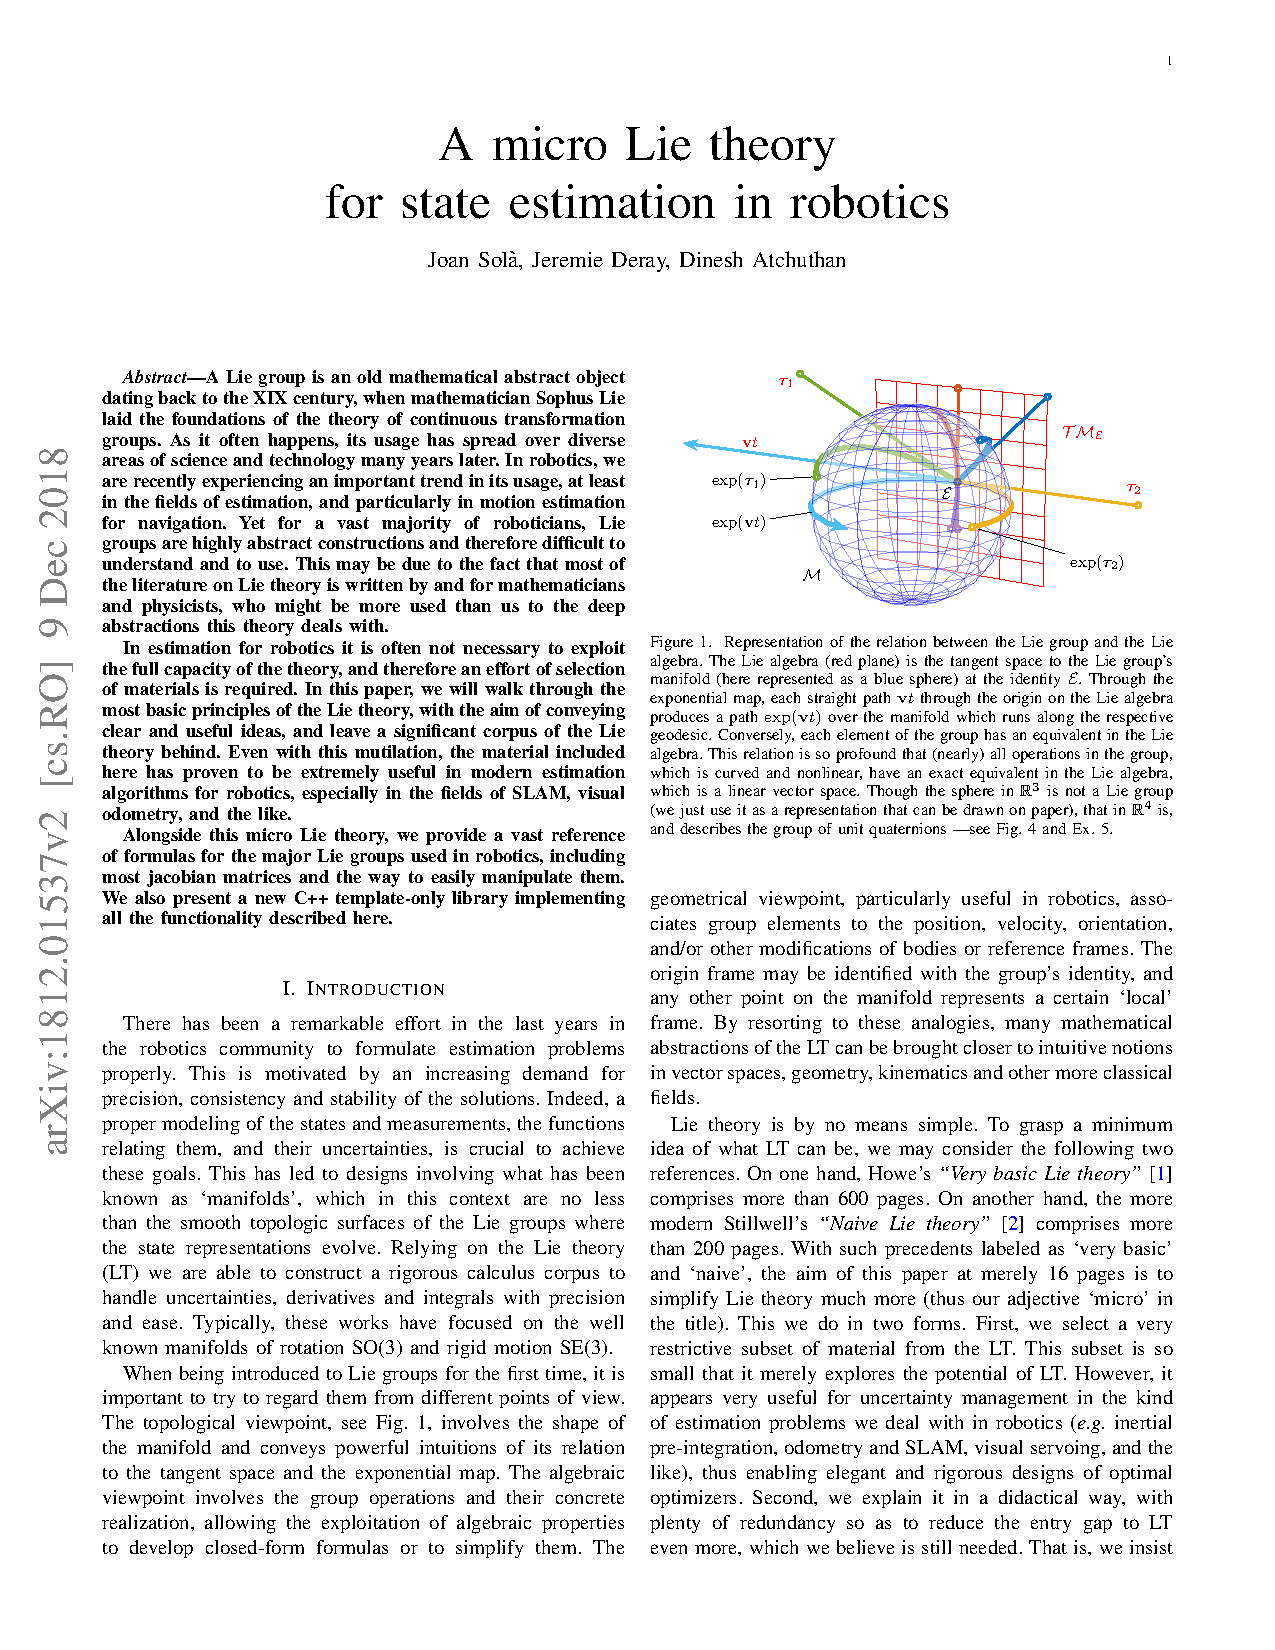
\includepdf[pages=-,scale=.8,pagecommand={}]{chap2_preliminaries/papers/micro_Lie_theory.pdf}



